%%%%%%%%%%%%%%%%%%%%%%%%%%%%%%%%%%%%%%%%%
% Masters/Doctoral Thesis 
% LaTeX Template
% Version 2.4 (22/11/16)
%
% This template has been downloaded from:
% http://www.LaTeXTemplates.com
%
% Version 2.x major modifications by:
% Vel (vel@latextemplates.com)
%
% This template is based on a template by:
% Steve Gunn (http://users.ecs.soton.ac.uk/srg/softwaretools/document/templates/)
% Sunil Patel (http://www.sunilpatel.co.uk/thesis-template/)
%
% Template license:
% CC BY-NC-SA 3.0 (http://creativecommons.org/licenses/by-nc-sa/3.0/)
%
%%%%%%%%%%%%%%%%%%%%%%%%%%%%%%%%%%%%%%%%%

%----------------------------------------------------------------------------------------
%	PACKAGES AND OTHER DOCUMENT CONFIGURATIONS
%----------------------------------------------------------------------------------------

\documentclass[
12pt, % The default document font size, options: 10pt, 11pt, 12pt
oneside, % Two side (alternating margins) for binding by default, uncomment to switch to one side
english, % ngerman for German
singlespacing, % Single line spacing, alternatives: onehalfspacing or doublespacing
%draft, % Uncomment to enable draft mode (no pictures, no links, overfull hboxes indicated)
%nolistspacing, % If the document is onehalfspacing or doublespacing, uncomment this to set spacing in lists to single
%liststotoc, % Uncomment to add the list of figures/tables/etc to the table of contents
%toctotoc, % Uncomment to add the main table of contents to the table of contents
%parskip, % Uncomment to add space between paragraphs
%nohyperref, % Uncomment to not load the hyperref package
headsepline, % Uncomment to get a line under the header
%chapterinoneline, % Uncomment to place the chapter title next to the number on one line
%consistentlayout, % Uncomment to change the layout of the declaration, abstract and acknowledgements pages to match the default layout
]{MastersDoctoralThesis} % The class file specifying the document structure

\usepackage[utf8]{inputenc} % Required for inputting international characters
\usepackage[T1]{fontenc} % Output font encoding for international characters

\usepackage{times} % Use the Palatino font by default

\usepackage[backend=bibtex,style=authoryear,natbib=true]{biblatex} % Use the bibtex backend with the authoryear citation style (which resembles APA)

\addbibresource{example.bib} % The filename of the bibliography

\usepackage[autostyle=true]{csquotes} % Required to generate language-dependent quotes in the bibliography
%----------------------------------------------------------------------------------------
%packages I ADDED  myself By Qiangsen
\usepackage{bm}
\usepackage{float}

\usepackage{graphicx}
\graphicspath{/Users/JohnsonJohnson/Downloads/thesis_1/Figures}
\usepackage{amsmath}

\renewcommand{\baselinestretch}{1.5}
%----------------------------------------------------------------------------------------

%----------------------------------------------------------------------------------------
%	MARGIN SETTINGS
%----------------------------------------------------------------------------------------

\geometry{
	paper=a4paper, % Change to letterpaper for US letter
	inner=2.5cm, % Inner margin
	outer=3.8cm, % Outer margin
	bindingoffset=.5cm, % Binding offset
	top=1.5cm, % Top margin
	bottom=1.5cm, % Bottom margin
	%showframe, % Uncomment to show how the type block is set on the page
}

%----------------------------------------------------------------------------------------
%	THESIS INFORMATION
%----------------------------------------------------------------------------------------

\thesistitle{Person re-identification based on and kernel local fisher discriminant analysis and Mahanalobis distance learning} % Your thesis title, this is used in the title and abstract, print it elsewhere with \ttitle
\supervisor{Professor Robert \textsc{Laganiere}} % Your supervisor's name, this is used in the title page, print it elsewhere with \supname
\examiner{} % Your examiner's name, this is not currently used anywhere in the template, print it elsewhere with \examname
\degree{Master of Applied Science} % Your degree name, this is used in the title page and abstract, print it elsewhere with \degreename
\author{Qiangsen \textsc{He}} % Your name, this is used in the title page and abstract, print it elsewhere with \authorname
\addresses{} % Your address, this is not currently used anywhere in the template, print it elsewhere with \addressname

\subject{Electrical Engineering and Computer Science} % Your subject area, this is not currently used anywhere in the template, print it elsewhere with \subjectname
\keywords{} % Keywords for your thesis, this is not currently used anywhere in the template, print it elsewhere with \keywordnames
\university{\href{http://www.university.com}{University of Ottawa}} % Your university's name and URL, this is used in the title page and abstract, print it elsewhere with \univname
\department{\href{http://department.university.com}{School of Electrical Engineering and Computer Science}} % Your department's name and URL, this is used in the title page and abstract, print it elsewhere with \deptname
\group{\href{http://researchgroup.university.com}{VIVA lab}} % Your research group's name and URL, this is used in the title page, print it elsewhere with \groupname
\faculty{\href{http://faculty.university.com}{Faculty of Engineering}} % Your faculty's name and URL, this is used in the title page and abstract, print it elsewhere with \facname

\AtBeginDocument{
\hypersetup{pdftitle=\ttitle} % Set the PDF's title to your title
\hypersetup{pdfauthor=\authorname} % Set the PDF's author to your name
\hypersetup{pdfkeywords=\keywordnames} % Set the PDF's keywords to your keywords
}

\begin{document}

\frontmatter % Use roman page numbering style (i, ii, iii, iv...) for the pre-content pages

\pagestyle{plain} % Default to the plain heading style until the thesis style is called for the body content

%----------------------------------------------------------------------------------------
%	TITLE PAGE
%----------------------------------------------------------------------------------------

\begin{titlepage}
\begin{center}

\vspace*{.06\textheight}
{\scshape\LARGE \univname\par}\vspace{1.5cm} % University name
\textsc{\Large Master's degree thesis}\\[0.5cm] % Thesis type

\HRule \\[0.4cm] % Horizontal line
{\huge \bfseries \ttitle\par}\vspace{0.4cm} % Thesis title
\HRule \\[1.5cm] % Horizontal line
 
\begin{minipage}[t]{0.4\textwidth}
\begin{flushleft} \large
\emph{Author:}\\
\href{http://www.johnsmith.com}{\authorname} % Author name - remove the \href bracket to remove the link
\end{flushleft}
\end{minipage}
\begin{minipage}[t]{0.4\textwidth}
\begin{flushright} \large
\emph{Supervisor:} \\
\href{http://www.jamessmith.com}{\supname} % Supervisor name - remove the \href bracket to remove the link  
\end{flushright}
\end{minipage}\\[3cm]
 
\vfill

\large \textit{A thesis submitted in fulfillment of the requirements\\ for the degree of \degreename}\\[0.3cm] % University requirement text
\textit{in the}\\[0.4cm]
\groupname\\\deptname\\[2cm] % Research group name and department name
 
\vfill

{\large \today}\\[4cm] % Date
%\includegraphics{Logo} % University/department logo - uncomment to place it
 
\vfill
\end{center}
\end{titlepage}

%----------------------------------------------------------------------------------------
%	DECLARATION PAGE
%----------------------------------------------------------------------------------------

\begin{declaration}
\addchaptertocentry{\authorshipname} % Add the declaration to the table of contents
\noindent I, \authorname, declare that this thesis titled, \enquote{\ttitle} and the work presented in it are my own. I confirm that:

\begin{itemize} 
\item This work was done wholly or mainly while in candidature for a research degree at this University.
\item Where any part of this thesis has previously been submitted for a degree or any other qualification at this University or any other institution, this has been clearly stated.
\item Where I have consulted the published work of others, this is always clearly attributed.
\item Where I have quoted from the work of others, the source is always given. With the exception of such quotations, this thesis is entirely my own work.
\item I have acknowledged all main sources of help.
\item Where the thesis is based on work done by myself jointly with others, I have made clear exactly what was done by others and what I have contributed myself.\\
\end{itemize}
 
\noindent Signed:\\
\rule[0.5em]{25em}{0.5pt} % This prints a line for the signature
 
\noindent Date:\\
\rule[0.5em]{25em}{0.5pt} % This prints a line to write the date
\end{declaration}

\cleardoublepage

%----------------------------------------------------------------------------------------
%	QUOTATION PAGE
%----------------------------------------------------------------------------------------

\vspace*{0.2\textheight}

\noindent\enquote{\itshape Thanks to my solid academic training, today I can write hundreds of words on virtually any topic without possessing a shred of information, which is how I got a good job in journalism.}\bigbreak

\hfill Qiangsen He

%----------------------------------------------------------------------------------------
%	ABSTRACT PAGE
%----------------------------------------------------------------------------------------

\begin{abstract}
\addchaptertocentry{\abstractname} % Add the abstract to the table of contents

Person re-identificaiton has become an intense research area in recent years. The main goal of this topic is to check if the individual appeared in other cameras is the same as the one in current cameras. This task is sometimes quite tough for the variation of illumination, camera angles, the passengers? clothes and object sheltering. It?s very important to choose robust descriptors and metric learning to improve accuracy. Ma- hanalobis based metric learning is a popular method to measure similarity. However, since directly extracted descriptors usually have high dimension, it's intractable to learn a high dimensional Mahanalobis matrix. Dimension reduction are used to project high dimensional descriptors to lower dimension space while preserving those discriminative information as much as possible. In this paper the kernel LFDA is used to reduce dimen- sion given that kernelization method can greatly improve re-identification performance for nonlinearity. Then a metric matrix is learned on lower dimensional descriptors based on the limitation that the within class distance is at least 1 unit smaller than the mini- mum inter class distance. This method turns to have excellent performance compared with other adcanced metric learning.
\end{abstract}

%----------------------------------------------------------------------------------------
%	ACKNOWLEDGEMENTS
%----------------------------------------------------------------------------------------

\begin{acknowledgements}
\addchaptertocentry{\acknowledgementname} % Add the acknowledgements to the table of contents
The acknowledgments and the people to thank go here, don't forget to include your project advisor\ldots
\end{acknowledgements}

%----------------------------------------------------------------------------------------
%	LIST OF CONTENTS/FIGURES/TABLES PAGES
%----------------------------------------------------------------------------------------

\tableofcontents % Prints the main table of contents

\listoffigures % Prints the list of figures

\listoftables % Prints the list of tables

%----------------------------------------------------------------------------------------
%	ABBREVIATIONS
%----------------------------------------------------------------------------------------

\begin{abbreviations}{ll} % Include a list of abbreviations (a table of two columns)

\textbf{LAH} & \textbf{L}ist \textbf{A}bbreviations \textbf{H}ere\\
\textbf{WSF} & \textbf{W}hat (it) \textbf{S}tands \textbf{F}or\\

\end{abbreviations}

%----------------------------------------------------------------------------------------
%	PHYSICAL CONSTANTS/OTHER DEFINITIONS
%----------------------------------------------------------------------------------------

%\begin{constants}{lr@{${}={}$}l} % The list of physical constants is a three column table
%
%% The \SI{}{} command is provided by the siunitx package, see its documentation for instructions on how to use it
%
%Speed of Light & $c_{0}$ & \SI{2.99792458e8}{\meter\per\second} (exact)\\
%%Constant Name & $Symbol$ & $Constant Value$ with units\\
%
%\end{constants}

%----------------------------------------------------------------------------------------
%	SYMBOLS
%----------------------------------------------------------------------------------------

\begin{symbols}{lll} % Include a list of Symbols (a three column table)

$a$ & distance & \si{\meter} \\
$P$ & power & \si{\watt} (\si{\joule\per\second}) \\
%Symbol & Name & Unit \\

\addlinespace % Gap to separate the Roman symbols from the Greek

$\omega$ & angular frequency & \si{\radian} \\

\end{symbols}

%----------------------------------------------------------------------------------------
%	DEDICATION
%----------------------------------------------------------------------------------------

\dedicatory{For/Dedicated to/To my\ldots} 

%----------------------------------------------------------------------------------------
%	THESIS CONTENT - CHAPTERS
%----------------------------------------------------------------------------------------

\mainmatter % Begin numeric (1,2,3...) page numbering

\pagestyle{thesis} % Return the page headers back to the "thesis" style

% Include the chapters of the thesis as separate files from the Chapters folder
% Uncomment the lines as you write the chapters

\chapter{Introduction}

People re-identification (Re-ID) has been an intense research topic in recent years, whose main goal is to match an image of a given person with other images of the same person. Person Re-ID has great potential in video surveillance, target detection and tracking and forensic search. However, it is quite challenging since the accuracy is much influenced by many factors like occlusion, illumination variation, camera settings and color response. In Re-ID, those images with known labels are called gallery images and the image used to know its label is called probe image. The probe image and gallery images can be from the same or different camera views, so the viewpoint and illumination between probe and gallery image can be quite different. Also because of the different color response of different cameras, the images of the same person may look different in different cameras. Besides, occlusions between camera and target person can also bring about quite much difficulty.  In a word, images of the same person may look different while images of different persons may kook quite the same. 

Given a sequence or video of individuals, there are three steps to match person. A simple work flow is shown in Figure \ref{workflow}. However, since most of used Re-ID datasets are already cropped manually or by a automatic detector, so most Re-ID work will only focus on robust descriptors designing and efficient matching algorithm designing aimed at those well cropped images. 


\begin{figure}[H]
\centering
%\begin{raggedleft}
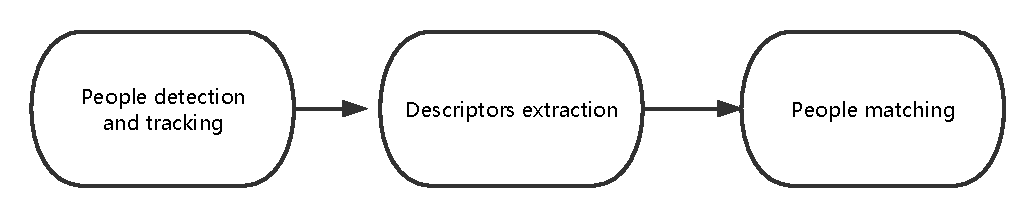
\includegraphics[scale = 0.7]{/Users/JohnsonJohnson/Downloads/thesis_1/Figures/REIDworkflow1.pdf}
%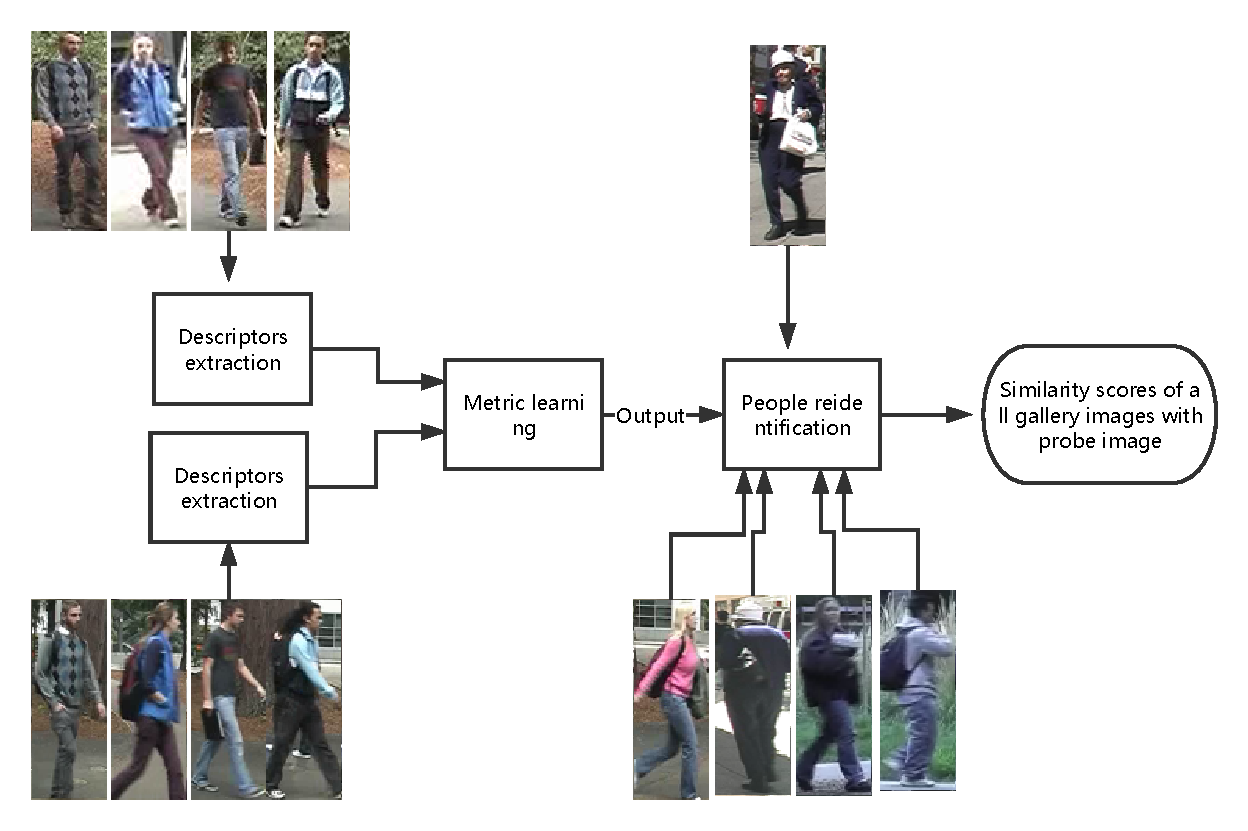
\includegraphics[width=1\linewidth]{REIDworkflow.pdf}
\vspace{1em}
\caption{Re-ID work flow}
%\end{raggedleft}
\end{figure}
\label{workflow}

\begin{figure}[H]
\centering
%\begin{raggedleft}
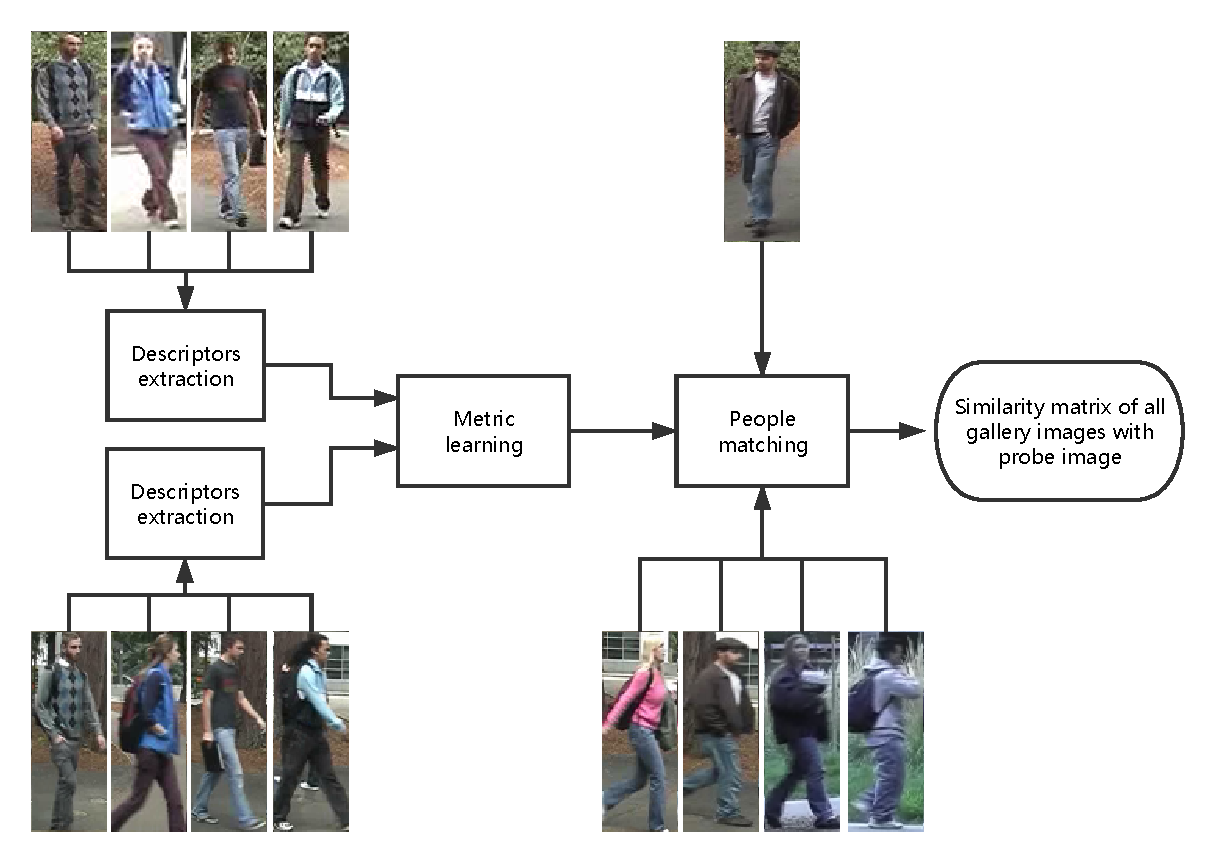
\includegraphics[scale = 0.7]{/Users/JohnsonJohnson/Downloads/thesis_1/Figures/REIDworkflow2.pdf}
%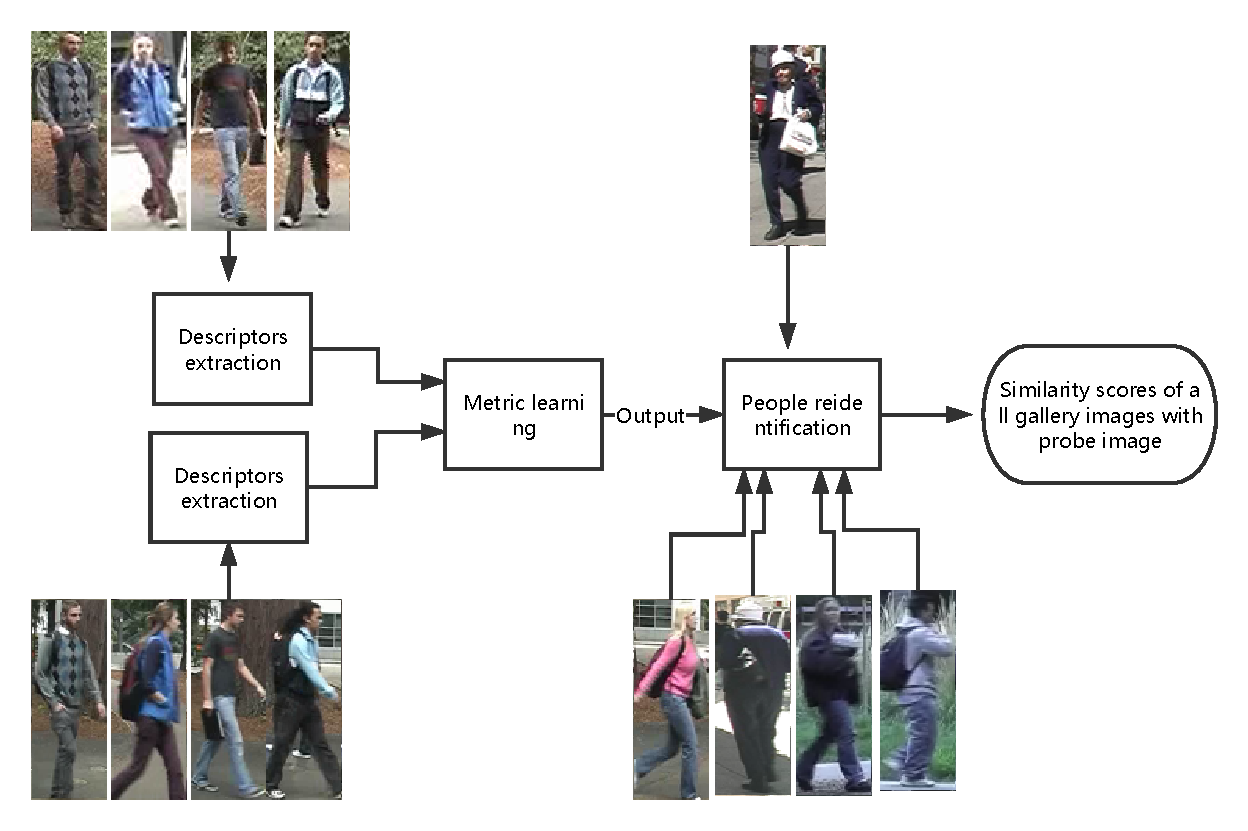
\includegraphics[width=1\linewidth]{REIDworkflow.pdf}
\vspace{1em}
\caption{A typical single shot Re-ID work flow}
%\end{raggedleft}
\end{figure}




The first task in Re-ID is to design a robust descriptor to represent images. The descriptor is supposed to contain the key information for each captured person. Basically, the descriptors are supposed to be robust and discriminative. One straightforward way is to extract the color, textural information of images, then the descriptors are used to compute the similarity score. But this method turns out to be not robust caused by illumination variation  and camera color response difference and camera angle settings.  Therefore, many other advanced descriptors takes into account the correlation of color, texture and position together to improve performance.

The second one is to design the similarity computing methodology. That is, the way to compare how similar two descriptors are. Previous methods use Euclidean distance, Bhattacharyya distance and Mahalanobis distance. The Euclidean distance is the easiest to match descriptors like color and texture descriptors but not the most effective. Many creative metric learning methods have been proposed to compute descriptor similarity. Among them the Mahanalobis distance based metric is most popular. The goal in Mahanalobis distance based metric is to learn a semi-positive definite (SPD) matrix $\bm{M}$ so that $\bm{M}$ satisfies predefined intraclass and interclass distance limitations.
	
\section{Basic concepts}
People re-identification can be divided into a few categories according to different conditions. Some general concepts are listed below.\\
\indent \textbf{Open set and close set Re-ID} \cite{REIDsurvey} According to the gallery size and how the gallery size evolves, Re-ID can be divided into open set Re-ID and close set Re-ID. In close set Re-ID, no new identities will be added to gallery set and gallery size remains the same as time goes by. Besides, the probe set will be a subset of gallery set, that means, the number of unique identities in gallery set will be equal or greater than probe set. In open set Re-ID, the gallery set will evolve as time goes by. Each time a probe image is inputed to the recognition system, the system will judge if it has a corresponding match in the gallery set. If the probe image doesn't match any of the gallery images, it will be regarded as a new identity and will be added to the gallery set. Besides, the probe set is not necessarily the subset of gallery set. 

\textbf{Long term and short term Re-ID} According to the time interval between gallery and probe images, Re-ID can be divided into long term and short term Re-ID.  In short term means the time interval between gallery and probe images are small, say a few minutes or several hours. In contrary, the long term Re-ID refers to the case that the time interval between gallery and probe images are a few days or even longer. The difference brought by long time interval between gallery and probe images is the variation of individuals' clothes and appearance. If the gallery images are shot a few days ago, the same individual may have changes his suits or take off his bag, then the appearance may change a lot. In this case, it will be much more difficult to recognize the same identity in long term Re-ID. Generally, in most cases we use the short term Re-ID, which guarantees the appearance of same person will remain the same and we only need to consider the difference brought by other factors like viewpoint variation and occlusions.


\textbf{Single shot and multi shot Re-ID} According to the size of sample set for each person, Re-ID can be divided into single shot and multi shots approaches. In single shot case, only one image is provided for a person in a camera view. Single shot Re-ID is challenging because only limited information can be extracted. One example is the VIPeR dataset Figure \ref{VIPeRimages}, in this dataset, for each person only one image is provides in each camera view and the viewpoint of each view is different. In multi shots Re-ID a sequence of images are provided for a person in a camera view. Compared with single shot case, more extra information, like temporal-spatial can be extracted from the sample set. One example of multi-shot dataset is the prid\_2011 dataset which provides a long sequence for each person in a single camera view.

%-------------------------------------------------
\begin{figure}[H]

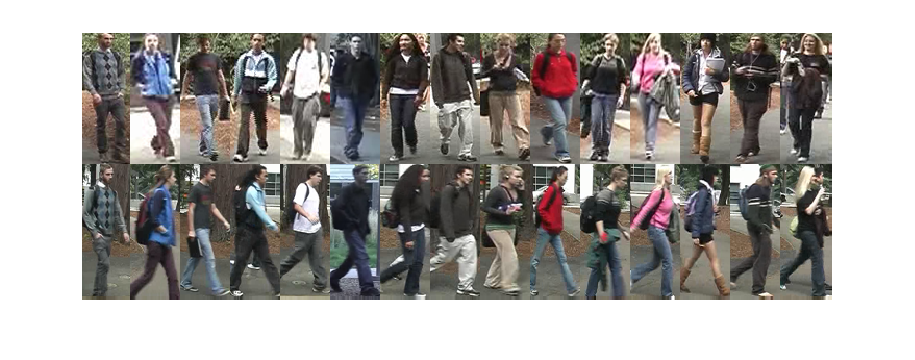
\includegraphics[width=1\linewidth]{/Users/JohnsonJohnson/Downloads/thesis_1/Figures/singleREID.eps}
\vspace{-3em}
\caption{The VIPeR dataset}
\label{VIPeRimages}
\end{figure}

%-------------------------------------------------

\begin{figure}[H]

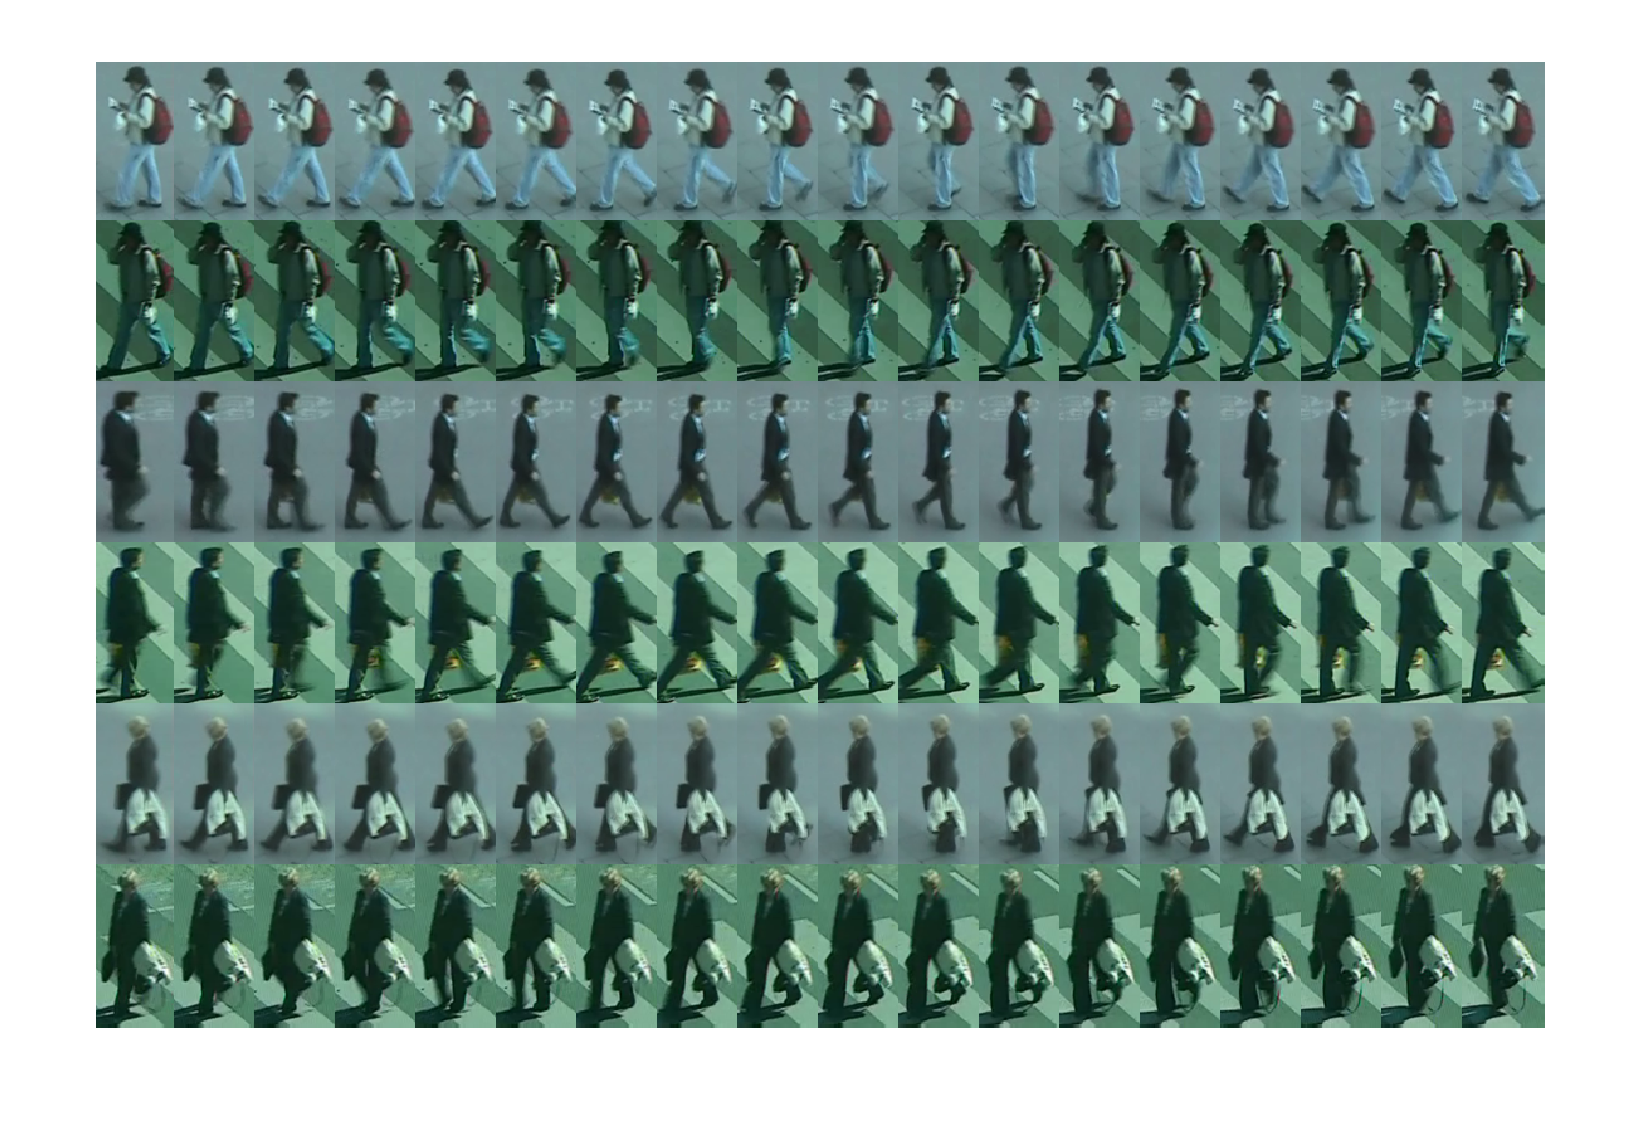
\includegraphics[width=1\linewidth]{/Users/JohnsonJohnson/Downloads/thesis_1/Figures/Multishots.eps}
\vspace{-3em}
\caption{Samples from prid\_2011 dataset}

\end{figure}


.

\section{Challenges}

\textbf{Detection, tracking and dataset labelling for supervised learning} Though classical person re-identification focus on descriptors designing and matching designing, in real-time application the detection and tracking has to be operated on video frames to get well cropped bounding box images. A good detection and tracking algorithm is necessary for Re-ID. Besides, training the matching algorithm is a supervised process, thus we have to know the labels for those training data. 

\textbf{Descriptors designing} Good descriptors should be robust to people pose variation, outer environment changes and camera settings. Though there have been many kinds of descriptors based on different property like color and texture, it is hard to judge which property is universally useful for different camera settings. In fact, the robustness, reliability and feasibility depends on different camera settings and viewing conditions. What's more, the pedestrian background may add much errors to descriptors, so it is important to quantify the impact of noisy background. Many works have tried to use segmented foreground of pedestrians, so it is important to design segmentation algorithms. The automatic foreground segmentation for single frame is difficult since there isn't that much available information compared with video background segmentation. Take VIPeR dataset as an example, there is only one frame for each view of a certain person, thus the segmented foreground masks are imperfect and chance is high that important body parts are lost. A segmented foreground provided by \cite{SDALF} is shown is Figure \ref{VIPeRFG}.
%-------------------------------------------------
\begin{figure}[H]
\centering
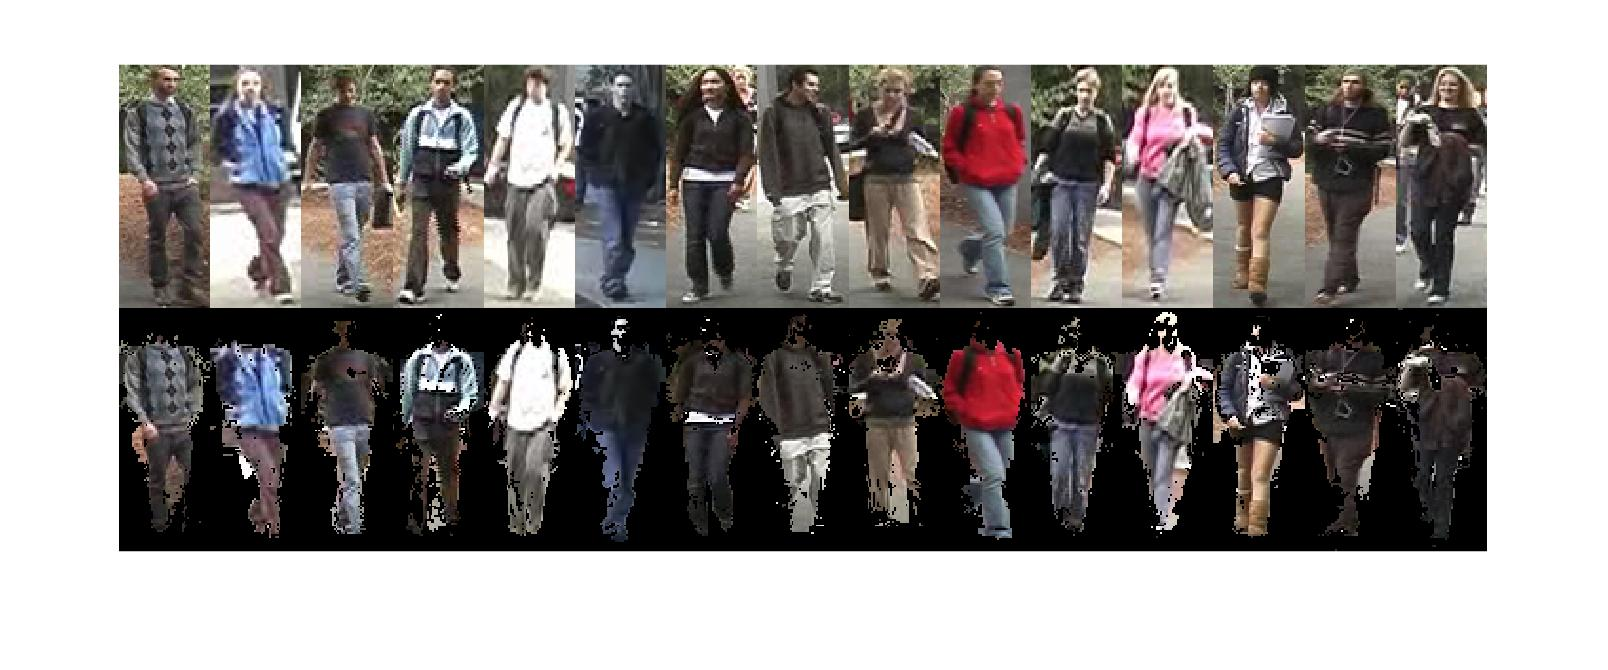
\includegraphics[width=1\linewidth]{/Users/JohnsonJohnson/Downloads/thesis_1/Figures/FGdemo.jpg}
\vspace{-3em}
\caption{VIPeR foreground}
\label{VIPeRFG}
\end{figure}

%-------------------------------------------------
\textbf{Efficient matching algorithm designing} 	
When designing machine learning algorithms to match persons, there are many limitations. One of them is the small sample size problem \cite{NFST}. The extracted descriptors usually has a high-dimensional $d$ but only a small number of sample $n(n<<d)$ size are available, underfitting may appear for insufficient data samples with high dimension. Besides, it is also necessary to take into consideration intra and inter distance of samples.
The intra distance means the distance of two samples with the same class label, while inter class distance is the distance of samples with different class labels. 

\textbf{Feasibility, Complexity and Scalability} When applying those descriptors and matching algorithms, we have to consider its real-time performance. The Re-ID datasets usually has small sample size but in surveillance network much more pedestrians in different cameras can be presented simultaneously. A system like this has plenty of individuals to re-identify, which requires the process time for single probe should be short for low latency. Besides, the since the gallery in this system evolves, it is crucial to design a evolution algorithm for gallery images, that is, how to judge if a person appeared in current camera is a new person to all those gallery images.

\section{Proposed work}
In many previous works, the kernel local fisher discriminant analysis is used as a subspace learning method, and Euclidean distance is usually used in the subspace to measure similarity. In this thesis, the KLFDA \cite{KLFDA} method is used a dimension reducing method to project high-dimensional descriptors to a lower-dimensional space. Compared with other dimension reduction methods, KLFDA is a supervised method and it takes consideration of those intra and inter class information, therefore, much less information are lost after dimension reduction. Then a Mahanalobis distance based matrix $M$ is learned based on the limitation that the distance of people from same class should be at least 1 unit smaller than the distance of people from different classes. A target function that penalizes large intra-class distance and small inter-class distance is created. When the target function converges by iterative computation, the matrix $\bm{M}$ is thought to be optimal. It turns out that this metric learning has good performance when compared with other metric learning methods. A workflow of proposed work is in Figure \ref{ProposedWorkflow}.

%------------------------------------------------------------
\begin{figure}[H]

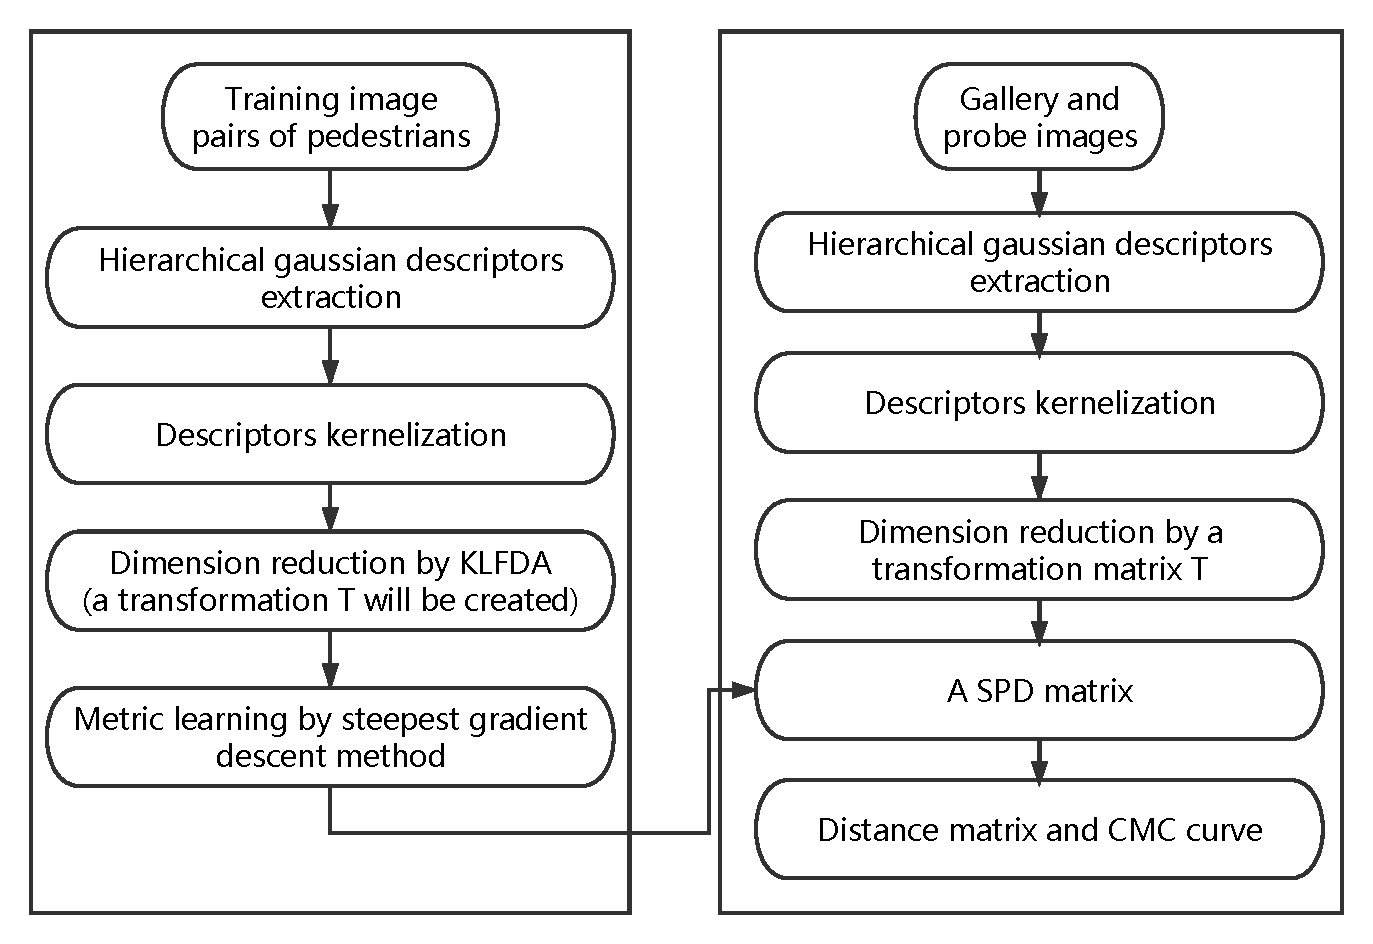
\includegraphics[width=1\linewidth]{/Users/JohnsonJohnson/Downloads/thesis_1/Figures/ProposedWorkFlow.pdf}
\vspace{-2em}
\caption{The workflow of proposed work, the left part is training and the right part is testing}
\label{ProposedWorkflow}

\end{figure}
%------------------------------------------------------------
\begin{figure}[H]

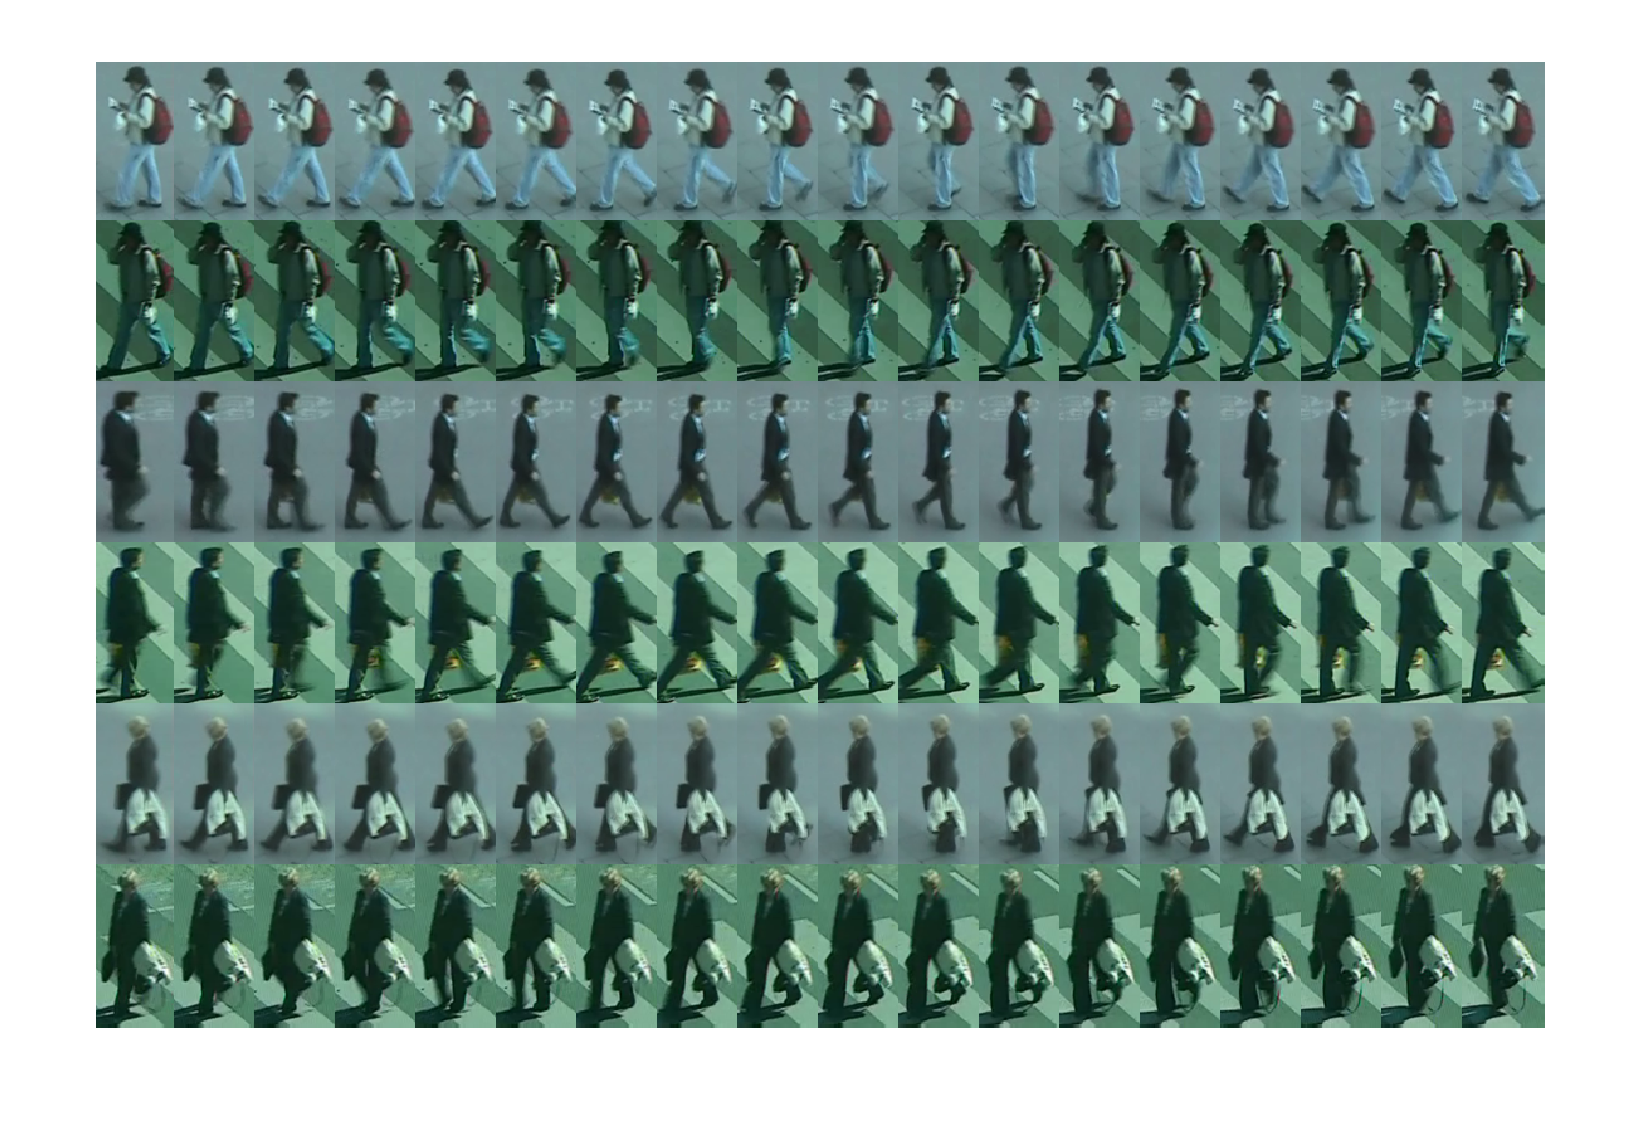
\includegraphics[width=1\linewidth]{/Users/JohnsonJohnson/Downloads/thesis_1/Figures/Multishots.eps}
\vspace{-2em}
\caption{Samples from prid\_2011 dataset}

\end{figure}


\section{Contributions}

In this paper we have three contributions, the first is that we combined the KLFDA with distance comparison learning. Instead of learning the subspace with KLFDA and computing Euclidean distance in a lower-dimensional space, a Mahanalobis distance based matrix is learned under the limitation that the within class distance is at least one unit smaller than inter class distance. Compared with those advanced metrics including cross view quadratic analysis(XQDA) \cite{LOMO} and Null space learning(NFST), this proposed metric learning proves to have excellent performance on VIPeR, CUHK1, prid\_2011, prid\_450s and GRID dataset.

Another contribution of this thesis is the influence of background subtraction on different descriptors is studied. We found that background subtraction can improve the performance of some descriptors (like HSV histogram) but can also decrease the performance of  other descriptors (texture feature like LBP and HOG). This comparison is shown in Chapter 3. The reason for this is that imperfect background segmentation brings in textural interference. If descriptors are color based and don't handle texture information, like HSV histogram descriptor, background segmentation can greatly improve the performance. However, if the descriptor extracts texture information, background segmentation will decrease its performance since the imperfect segmentation will mask out many parts of the foreground area, which will cause important textural information variation. Because segmentation algorithm will cause different influence on various features, in this thesis, a weighted map of images is used instead of using the background segmentation.

The last one is some variants of hierarchical gaussian descriptor have been tested. Local binary pattern (LBP) is used in basic pixel feature. Superpixel segmentation is also applied to combine with hierarchical gaussian descriptor, which implies overlapping patch sampling is important in hierarchical gaussian. At last, Gaussian mixture model (GMM) is also tested but only gets worst performance.

\section{Thesis organization}
In this thesis, Chapter 2 will give a brief introduction of previous work. Chapter 3 will explain the implementation of the hierarchical gaussian descriptors used in this thesis. The performance of some variants of hierarchical gaussian is studied in this Chapter. In Chapter 4 a detailed introduction of the kernel local fisher local discriminant analysis will be presented, and a detailed explanation will also be presented about the metric learning on the lower-dimensional space based on relative distance limitation learning.
In Chapter 5 the used datasets and parameters and other experiment settings will be explained, and a detailed analysis of results is presented here. At last, the conclusion is given in Chapter 6.





\chapter{Related work}
Previous works mainly focus on finding more discriminative descriptors and better metric learning. It is known that color and texture are the most important information in Re-ID. Researchers found that features based on a single attribute (like color or texture) are not robust to various datasets. Instead, combinations of different features are exploited to improve the performance. Most descriptors capture the local or global statistic color and texture information to characterize individuals. A brief introduction of those descriptors and metrics is given in this chapter.

\section{Appearance descriptors}
In most descriptors, the input image will be divided into a few subregions to model the complex human kinematics. Features of those subregions are extracted respectively and concatenated directly or characterized by their statistic properties. According to how those subregions are divided, there can be three kinds of models, fixed part-based models, adaptive models and learned part models \cite{Appearancedesc}. 

In fixed part models, the size of body parts is predefined. One example is in \cite{ImportantFeatures, PRDC, REIDSVM}, where a silhouette is divided into a fixed number of horizontal stripes, which mainly include the head, torso and legs. In \cite{AppBasedREID}, the input images are divided into three horizontal stripes, and the width of each stripe is respectively 16\%, 29\% and 55\%.  The fixed models predefine parameters such as numbers of stripes and the stripe height. 

In the adaptive part models, the size of each body parts may vary to fit predefined body part models. Take \cite{SDALF} for an instance; the silhouette of each person is divided into three parts horizontally, which include the head, torso and legs respectively. But the height of each stripe is different for various silhouettes, and it is computed according to symmetry and asymmetry with two operators $C(i, \delta)$ and $S(i,\delta)$, where 
\begin{equation}
\begin{aligned}
C(i,\sigma) & = \sum_{B_{[i-\delta, i+\delta]}}{d^2(p_i-{\hat{p}_i)}}, \\
S(i,\sigma) &= \sum{\frac{1}{W\delta}|A(B_{[i,i-\delta]}) - A(B_{[i,i+\delta]})|}.
\end{aligned}
\end{equation}
Here the $C(i, \delta)$ is called the \emph{chromatic bilateral operator}, and it computes the Euclidean distance of two HSV blobs located symmetrically with respect to horizontal axis $y = i$, where $B_{[i-\delta, i+\delta]}$ is the blob with a height $2\delta$. $S(i,\delta)$ is called the \emph{spatial covering operator} and it computes the difference of two foreground areas. Then the axis between the torso and legs is computed as follow:
\begin{equation}
\begin{aligned}
i_{TL} = \mathop{\arg\min}_i(1-C(i,\delta)+S(i,\delta)),
\end{aligned}
\end{equation}
and the axis  between the head and torso is computed with the following equation:
\begin{equation}
\begin{aligned}
i_{HT} = \mathop{\arg\min}_i(-S(i,\delta)).
\end{aligned}
\end{equation}
The axis dividing the left and right torso is
\begin{equation}
\begin{aligned}
j_{LR} = \mathop{\arg\min}_j(C(j,\delta)+S(j,\delta)).
\end{aligned}
\end{equation}
This method has good performance. But one shortcoming of this model is that an imperfect background segmentation causes noise and introduces errors regarding the position of axes. \\
%-------------------------------------------------------------------------------------------------------------------------------------------------------------------------------------------------------------------------------------------------------------------
\indent Another part-based adaptive spatial-temporal model used in \cite{PartbasedSTReid} characterizes a person's appearance using color and facial features. Few works exploit human face features. In this work, human face detection based on low resolution cues selects useful face images to build face models. Color features capture representative color as well as the color distribution to build a color model. This model handles multi-shot re-identification, and it also characterizes the color distribution variation of many consecutive frames.  Besides, the facial features of this model is conditional. That is, in the absence of good face images, this model is only based on color features.

Some methods based on learned part models have been proposed. Part model detectors (statistic classifiers) are trained with manually labelled human body parts images, exploiting features related to edges contained in the images. A pictorial structure (PS) is proposed in \cite{PictorialModel}. The PS model of a non-rigid body is a collection of part models with deformable configurations and connections with certain parts. The appearance of each part is separately modelled, and deformable configurations are implemented with spring-like connections. This model can quantitatively describe visual appearance and model the non-rigid body. In \cite{PSmodelRevisit}, the pictorial structure body model is made up of N parts and N corresponding part detectors. 

Another example of the learned part model is in \cite{MultiPersonREID, PartbasedSTReid}. The overall human body model consists of several part models; each model is made up of a spatial model and a part filter. For each part, the spatial model defines allowed arrangements of this part with respect to the bounding box. To train each model, the latent support vector machine (LSVM) is used, and four body parts are detected, namely the head, left and right torso and upper legs. Compared with other models, this model exploits a sequence of frames of an individual and thus captures appearance characteristics as well as the appearance variation over time.

Features can be implemented with different methods. According to the way to extract features for a model (a whole model or a part-based model), features can be divided into two categories: global and local features. Global features refer to features extracted from a whole image or region, and the size of the descriptor is usually fixed. In order to extract local feature of a specified image or region, we first divide the whole image into many equal blocks and compute the feature of each block.  Both descriptors may deal with color, texture and shape. The color information is exploited most by extracting the color histogram within different color spaces. Descriptors based on texture, such as the scale-invariant feature transform (SIFT), speeded up robust features (SURF) and LBP, are also widely combined to improve performance.

Global color histogram is a frequently used global feature. For an three-channel image, like an RGB image, each channel is quantized into $B$ bins separately. The final histogram could be a multi-dimensional or one-dimensional histogram. For instance, if $B = 8$, for a multi-dimensional histogram, there will be  $8\times 8\times 8 = 512$ bins. But if we concatenate the three-dimensional bins together, the dimension can be reduced to $8 + 8 + 8 = 24$ bins while the performance of this reduced descriptor doesn't decrease. This method can be applied on other color spaces like HSV and Lab, etc.

Local color histogram usually splits the specified model or region into many equal-sized blocks and computes the global feature of each block. The feature can be based on color, texture and interest points. SIFT \cite{SIFT} is a kind of local feature based on the interest points. The salient interest points (identifiable over rotating and scaling) are selected by the interest operator. This algorithm detects key points by computing the difference of Gaussian ($DoG$) images of different scales $\sigma$ with the equation
\begin{equation}
D(x,y,\sigma) = (G(x,y,k_1\sigma) - G(x,y,k_2\sigma))\ast I(x,y).
\end{equation}
Here $G(x,y,k_1\sigma)$ is the Gaussian function with deviation $k_1\sigma$, $I(x,y)$ is the image. The $DoG$ images are compared to find their extrema as key points. With key points localization and other processing, descriptors describing key points are created as SIFT descriptors.

The maximally stable color region (MSCR) is used in \cite{SDALF}. The MSCR derives from the maximally stable extreme region (MSER) and detects the region with a stable color cluster. It uses an agglomerative clustering algorithm to compute color clusters, and by looking at the successive time steps of the algorithm, the extension of color is implemented. The detected color region is described with a nine-dimensional vector containing the area, averaging color, centroid and second moment matrix. With this vector, the color region detected makes it easy to do scale and affine transforms.

Recurrent highly structured patches (RHSP) is also used in \cite{SDALF}. This feature captures patches with highly recurrent color and texture characteristics from extracted silhouette pixels. This feature is extracted from the following steps. First, random and probably overlapping small image patches are extracted from silhouette pixels. Then, to capture those patches with informative texture, the entropy of each patch (the sum of the three channels' entropy) is computed, and we discard those patches with entropy smaller than a specified threshold. In the next step, some transforms are performed on the remaining patches to select those remaining invariant to the transforms. Subsequently, the recurrence of each patch is evaluated with the local normalized cross correlation (LNCC) function. This evaluation is only performed on a small region containing the patch instead of the whole image. Then the patches with high recurrence are clustered to avoid patches with similar content. Finally, the Gaussian cluster is applied to maintain the patch nearest to the centroid of each cluster for each cluster.

In \cite{SARC3D}, a new 3D model model called SARC3D  is used to characterize the individual. Compared with those 2D models, this model combines the texture and color information with their location information together to get a 3D model. This model starts with an approximate body model with a single shape parameter. By precise 3D mapping, this parameter can be learned and trained with even quite few images (even one image is feasible). This model's construction is driven by the frontal, top and side views extracted from various videos, and for each view, the silhouette of a person is extracted to construct the 3D graphical model. The final body model is sampled to get a set of vertices from the previously learned graphic body model. Compared with other models, this model has a robust performance when dealing with partial occlusion, people posture variation and viewpoint variations since the model is based on silhouettes from three viewpoints.
%--------------------------------------------------------------------------------------------------------------------------------------------------------------------------------------------------------------------------------------------------------------------------------

Descriptors combining color and texture are most often used in re-identification. In \cite{AHPE}, a signature called asymmetry-based histogram plus epitome (AHPE) was proposed. This work starts with a selection of images to reduce image redundancy, which is caused by correlated consecutive sequences. This descriptor combines global and local statistical descriptors of human appearance, focusing on overall chromatic content via histogram and on the recurrent local patches via epitome analysis. Similar to the SDALF descriptor \cite{SDALF}, the HPE descriptor consists of three components, the chromatic color histogram, the generic epitome and local epitome. The chromatic color histogram is extracted in the HSV color space, which turns to be robust to illumination changes. Here, color histogram is encoded into a 36-dimensional feature space $[H=16,  S=16,  V=4]$. The authors define epitome to be a collage of overlapped patches. This collage is generated by the collapsing of an image or a sequence of images, and this collage indicates the essence of the texture, shape and chromatic properties of the image or sequential images.

\section{Metric learning}
The second step of Re-ID is to design the metric learning to match descriptors, i.e., the way to compare how similar two descriptors are. Many different metric learning methods have been proposed \cite{KISSME, LFDA, PCCA, TDL, PRDC, LMNN, KLFDA, KCCA, KernelVersionMetrics, NFST, ITML} to get smaller intraclass distance and larger interclass distance. Generally, for two $d\times 1$-dimensional input vectors $\bm{x}_1$, $\bm{x}_2$, any symmetric positive semi-definite matrix $M$ defines a pseudo-metric with the form of $D = (\bm{x}_1 -\bm{x}_2)^T\bm{M}(\bm{x}_1 - \bm{x}_2)$. Many widely used distance metrics exploit this rule. Previous methods includes the Euclidean distance, Bhattacharyya distance and Mahalanobis distance methods. The Euclidean distance, which is the most common used distance, is a special case of Mahalanobis distance when the $\bm{M}$ is an identity matrix. One example of metric learning is the probabilistic relative distance comparison model proposed in \cite{PRDC}. This model exploits all the possible positive person pairs and negative pairs so that for each person, the between-class distance is larger than the within-class distance. Compared with the other distance learning models proposed, this model solves the matrix $\bm{M}$ by an iterative optimization algorithm. Suppose $\bm{z}$ is an image descriptor of a person; the task is to identify another image descriptor $\bm{z}'$ of the same person from $\bm{z}''$ of a different person by using a distance model $f(\cdot)$, so that $f(\bm{z}, \bm{z}')< f(\bm{z}, \bm{z}'')$. The authors convert the distance learning problem to a probability comparison problem by measuring the probability of the distance between a relevant pair of images being smaller than that of a related irrelevant pair as
\begin{equation}
P(f(\bm{z},\bm{z}')<f(\bm{z},\bm{z}'')) = (1+\exp^{(f(\bm{z}-\bm{z}')-f(\bm{z}-\bm{z}''))})^{-1}.
\end{equation}
Here the author assumes that probability of $f(\bm{z},\bm{z}')$ and $f(\bm{z},\bm{z}'')$ is independent, therefore, using the maximal likelihood principal, the optimal function can be learned as
\begin{equation}
\begin{aligned}
f &= \mathop{\arg\min}_f r(f,O), \\
r(f,O) &= -\log(\prod_{O_i}P(f(\bm{x}_i^p) < f(\bm{x}_i^n))).
\end{aligned}
\end{equation}
$O=\{O_i=(\bm{x}_i^p, \bm{x}_i^n)\}$ , $\bm{x}_i^p$, $\bm{x}_i^n$ are intraclass and interclass vector differences respectively, and $\bm{x}_i^p$, $\bm{x}_i^n$ are defined as
\begin{equation}
\begin{aligned}
\bm{x}_i^p &= |\bm{z} - \bm{z}'|, \\
\bm{x}_i^n &= |\bm{z} - \bm{z}''|.
\end{aligned}
\end{equation}
The distance function $f(\cdot)$ here is parameterized as the Mahalanobis distance function
$f=\bm{x}^T\bm{M}\bm{x},\bm{M\ge}0$. Here $\bm{M}$ is a semi-positive definite (SPD) matrix. In this way, the distance function learning problem is transformed to a matrix optimization problem. The author used an iteration algorithm to compute matrix $\bm{M}$. One shortcoming for this algorithm is that it is computationally expensive because for each person it compares distances between all the possible negative pairs and corresponding positive pairs. 

Single-shot image-based person representation suffers from the small sample size problem. This is why multi-shot Re-ID has been proposed. Since there are a sequence of images for each individual, there are many more cues to exploit.
In \cite{TDL}, the author simplified computing of the Mahananobis matrix by applying the new limitations on datasets. The author found that when using video-based person representation, the difference of interclass may be more obscure than that of still-image-based representation. Therefore, the author proposed the top-push distance learning model. For all the person pairs, the maximal intraclass distance should be one unit smaller than the minimal distance of interclass distance. Another constraint introduced the sum of all intraclass distance should be as small as possible, so the final target function is summarized as:
\begin{equation}
\begin{aligned}
f(D) = (1-\alpha)\sum_{\bm{x}_i,\bm{x}_j,y_i=y_j} D(\bm{x}_i,\bm{x}_j) + \\
\alpha \sum_{\bm{x}_i,\bm{x}_j,y_i=y_j}\max\{{D(\bm{x}_i,\bm{x}_j)-\min_{y_i\ne y_k}{D(\bm{x}_i,\bm{x}_k)}+\rho,0}\}.
\end{aligned}
\end{equation}
Here, $\bm{x}_i, \bm{x}_j and \bm{x}_k$ are feature descriptors, and $y_i, y_j and y_k$ are class labels.

Some previous works exploit the Fisher discriminant analysis and convert the problem to a matrix eigenvalue decomposition problem. In \cite{LFDA}, the local fisher discriminant analysis (LFDA) is used, and in \cite{KernelVersionMetrics}, the kernel version of several linear metrics are proposed, and it proves that kernelization improves Re-ID performance. In \cite{LOMO}, the log ratio of Bayesian-based estimation is proposed to have advanced performance. In \cite{NFST}, the authors propose to make sample points of the same class collapse to the same point in the null space while different points are project to different points. In \cite{SCNCD}, the semantic representation of color names is exploited. In this thesis, an SPD matrix $\bm{M}$ is learned to meet certain intraclass and interclass distance limitations. 

\section{Other methods for Re-ID}
Besides the descriptors and metrics mentioned above, there are some other methods for Re-ID. Convolutional neural networks (CNN) have been exploited in Re-ID. One advantage of the neural network Re-ID is that the preprocessing of images can be skipped. We can also say the preprocessing is included in convolutional layers. The input of this structure can be straightforward grey images or color images.  Traditional neural networks have too many weights to train. Convolutional neural networks can avoid this problem while retaining high performance. Compared with classical neural network architecture, the convolutional neural network exploits receptive field, weights sharing and pooling to reduce weights number and thus decreases computational cost. When dealing with multi-shot and video-based re-identification, neural networks are proven to have better performance. In \cite{RecurrentCNN}, the author proposes a recurrent neural network layer and temporal pooling to combine all time-steps data to generate a feature vector of the video sequence. In \cite{MultiCNN}, the author proposes a multi-channel layer based neural network to jointly learn both local body parts and whole body information from input person images.  In \cite{DeepfeatureCNN}, a convolutional neural network learning deep feature representations from multiple domains is proposed, and this work also proposes a domain-guided dropout algorithm to dropout CNN weights when learning from different datasets. \\
\indent There are many other works based on convolutional neural networks. However, person re-identification may be one of the areas where CNN performance may be poorer than regular machine learning methods for the small sample size problem (SSS). In most datasets, the sample size of each pedestrian is quite small. Especially in single-shot Re-ID only one frame is provided in each view for each person. This is why Re-ID more often relies on classical machine learning.

%
%By learning from multiple datasets this method gives a solution to the problem that most CNNs are not trained enough caused by datasets with small number of images.

\section{Some state-of-the-art works}
Recently, many works have been proposed that improved Re-ID performance by a wide margin. In this section, those advanced descriptors and metrics are introduced. 

\textbf{Cross view quadratic discriminant analysis} (XQDA) is proposed in \cite{LOMO}. Let's define the sample difference $\Delta = \bm{x}_i - \bm{x}_j$, where $\bm{x}_i $ and $\bm{x}_j$ are two feature vectors. $\Delta$ is called intrapersonal difference when their labels satisfy $y_i = y_j$ and extrapersonal difference when $y_i \ne y_j$. The intrapersonal and interpersonal variation can be defined as $\Omega_I$ and $\Omega_E$. The authors convert the Re-ID problem to distinguishing $\Omega_I$ from $\Omega_E$. In \cite{Bayeface}, each one of intrapersonal and interpersonal class is modelled with a multivariate Gaussian distribution, and in \cite{Bayeface}, it has been proven that both $\Omega_I$ and $\Omega_E$ have zero mean. Under the zero-mean distribution, the probability of observing $\Delta$ in $\Omega_I$ and the probability of observing $\Delta$ in $\Omega_E$ can be denoted as
\begin{equation}
\begin{aligned}
P(\Delta|\Omega_I) &= \frac{1}{(2\pi)^{d/2}|\Sigma_I|^{1/2}}\exp^{\frac{-1}{2}\Delta^T\Sigma_I^{-1}\Delta},\\
P(\Delta|\Omega_E) &= \frac{1}{(2\pi)^{d/2}|\Sigma_E|^{1/2}}\exp^{\frac{-1}{2}\Delta^T\Sigma_E^{-1}\Delta},
\end{aligned}
\end{equation}
where $\Sigma_I$ and $\Sigma_E$ are the covariance matrix of $\Omega_I$ and $\Omega_E$. Then the probability ratio between the interpersonal pairs and intrapersonal pairs can be denoted as
\begin{equation}
\begin{aligned}
r(\Delta) = \frac{P(\Delta|\Omega_E)}{P(\Delta|\Omega_I)}
	   &=\frac{\frac{1}{(2\pi)^{d/2}|\Sigma_E|^{1/2}}\exp^{\frac{-1}{2}\Delta^T\Sigma_E^{-1}\Delta}}{\frac{1}{(2\pi)^{d/2}|\Sigma_I|^{1/2}}\exp^{\frac{-1}{2}\Delta^T\Sigma_I^{-1}\Delta}},\\
r(\Delta)& =  C\exp^{\frac{-1}{2}\Delta^T(\Sigma_E^{-1} - \Sigma_I^{-1})\Delta}.
\end{aligned}
\end{equation}
Here C is a constant term, and by taking the log and deserting the constant term, we have 
\begin{equation}
\begin{aligned}
r(\Delta) = \Delta^T(\Sigma_I^{-1} - \Sigma_E^{-1})\Delta 
	   & = (\bm{x}_i - \bm{x}_j)^T(\Sigma_I^{-1} - \Sigma_E^{-1})(\bm{x}_i - \bm{x}_j).
\end{aligned}
\end{equation}
In \cite{LOMO}, a subspace $W$ is learned so that 
\begin{equation}
r(\Delta) = (\bm{x}_i - \bm{x}_j)^TW({\Sigma_I}'^{-1} - {\Sigma_E}'^{-1})W^T(\bm{x}_i - \bm{x}_j),
\end{equation}
and ${\Sigma_I}' = W^T\Sigma_IW, {\Sigma_E}' = W^T\Sigma_EW$. Therefore, a subspace $M(W) = W({\Sigma_I}'^{-1} - {\Sigma_E}'^{-1})W^T$ is learned in this work.\\
\indent \textbf{Null Foley-Sammon transform (NFST)} In \cite{NFST}, a null space is proposed so that with this space the intraclass points collapse to a same point in the null space while interclass points are projected to different points. Given the within-class scatter $\bm{S}^w$ and between-class scatter $\bm{S}^b$, an optimal projection matrix $\bm{W}$ is computed so that 
\begin{equation}
\begin{aligned}
\bm{w}_i^T\bm{S}^w\bm{w}_i = 0,\\
\bm{w}_i^T\bm{S}^b\bm{w}_i > 0.
\end{aligned}
\end{equation}
Here $\bm{w}_i$ is the $i_{th}$ column in $\bm{W}$.

It can be noted that like many other metric learnings, XQDA and NFST evolve to matrix decomposition and eigenvalue selection problems. In this paper, XQDA and NFST are used to compare with the proposed metric. In \cite{GOG}, it has been shown that GOG + XQDA outperforms many other combinations, including MetricEnsemble \cite{MetricEnsembles}, SCNCD \cite{SCNCD}, SemanticMethod \cite{SemanticMethod}, etc. In \cite{ NFST}, it has been shown LOMO + NFST outperforms metrics including LMNN \cite{LMNN}, KCCA \cite{KCCA}, ITML \cite{ITML}, KLFDA \cite{KLFDA}, MFA \cite{KernelVersionMetrics}, KISSME \cite{KISSME}, SimilarityLearning \cite{SimilarityLearning}, SCNCD \cite{SCNCD}, Mid-level Filters \cite{MidlevelFilters} and Improved Deep \cite{ImprovedCNN}. Based on the result that XQDA and NFST outperform other metrics, XQDA and NFST are used in this thesis to compare with our proposed metric learning. 

\section{Performance measuring}
There are a few measures of Re-ID, such as cumulative matching curve (CMC), receiver operating characteristic curve (ROC) and synthetic recognition rate (SRR). Specifically, the CMC is used as a 1:m re-identification system and ROC is used for a 1:1 re-identification system. The
SRR curve indicates the probability that any of given fixed number of matches is correct.

For the open-set Re-ID problem, the ROC \cite{PartbasedSTReid, MultiPersonREID} curve is adopted. The ROC represents the relationship between Re-ID accuracy vs the false accept rate (FAR). In the ROC the x-axis is the FAR and the y-axis is the accuracy. Re-ID accuracy and the FAR are defined by equations
\begin{equation}
\begin{aligned}
Accuracy = \frac{TPs}{N_p},\\
FAR = \frac{MMs + FPs}{N_p}.
\end{aligned}
\end{equation}
The true positives (TPs) are the number of probe IDs that are correctly accepted. $N_p$ is the number of all positive probes. The FAR is expressed by the mismatches (MMs), false positives (FPs) and N$_\text{p}$. MMs are those probe IDs that are incorrectly matched to the galley set when in fact those probe IDs exist in the gallery. The FPs are the number of probe IDs incorrectly matched to the gallery when they don't actually exist in the gallery. 

For the closed-set Re-ID problem, the most commonly used performance measuring is the CMC. Closed-set Re-ID assumes that the probes are contained in the gallery set, and the performance is measured by ranking the gallery with respect to each probe. The CMC describes the probability of the right match given a list of computed similarity scores, and the first ranked ID is regarded as the matched individual.

The proportion of uncertainty removed (PUR) is proposed in \cite{LFDA}. PUR measures the entropy difference between before ranking and after ranking. For a certain probe before ranking, all those samples in the gallery set have equal probability, and the entropy is $\log(S)$, $S$ being the number of observations in gallery set. After ranking, the entropy is $\sum M(r)\log(M(r))$, and $M(r)$ is the probability that the right match is within the top $r$ ranked observations. With normalization, the PUR value is computed by the equation
\begin{equation}
PUR = \frac{\log(S)-\sum M(r)\log(M(r))}{\log(S)}.
\end{equation}

In this thesis, the CMC is used to measure Re-ID performance because most datasets are tested under closed-set Re-ID settings. In this metric, the $CMC(k)$ stands for the probability that the right match is within the top k matches. Suppose a set of gallery $G = \{G_1,G_2,\cdots,G_m\}$ and a set of probe $P = \{P_1,P_2,\cdots,P_n\}$, for each identity $P_i$, there should be a right match in the gallery set. However, there could be identities that appear in the gallery set but not in the probe set. A $m\times n$ similarity matrix can be computed. Then for each probe identity $P_i$, a sorted list of gallery identities can be list as $S(P_i) = \{{G_{(1)},G_{(2)},\cdots,G_{(m)}}\}$ so that their similarity with $P_i$ descends. Suppose the right match of $P_i$ is at the position $k$ of $S(P_i)$, $k\le m$, then $G_i$ has a rank value of $k$. Therefore, the CMC can be calculated as 
\begin{equation}
CMC(k) = \frac{1}{n}(\#k_l\le k),
\end{equation}
where $k_l$ is the list of rank values of $P = \{P_1,P_2,\cdots,P_n\}$, and $\#k_l\le k$ means the number of rank values that are smaller than k.  Therefore, the CMC curve always ascends and converges at 1.  A perfect CMC is supposed to have a hight rank 1 score and approaches 1 as fast as possible.

An example of CMC computing is as follows. Suppose the gallery size is $M=10$ and the probe size is $N=15$. By computing the similarity and ranking them, we have a rank score frequency table such  as that shown in Table \ref{CMCcomputingdemo}.
\begin{table}[H]
\centering
\caption{A CMC example of gallery size is $M=10$ and probe size is $N=12$}
\label{CMCcomputingdemo}
\begin{tabular}{|l|c|c|c|c|c|c|c|c|c|c|c|c|}
\hline
RankScore &1&2&3&4&5&6&7&8&9&10&11&12\\
\hline
Frequency &5&3&2&1&1&0&0&0&0&0&0&0\\
\hline
CumulativeSum&5&8&10&11&12&12&12&12&12&12&12&12\\
\hline
\end{tabular}
\end{table}

\begin{figure}[H]
\centering
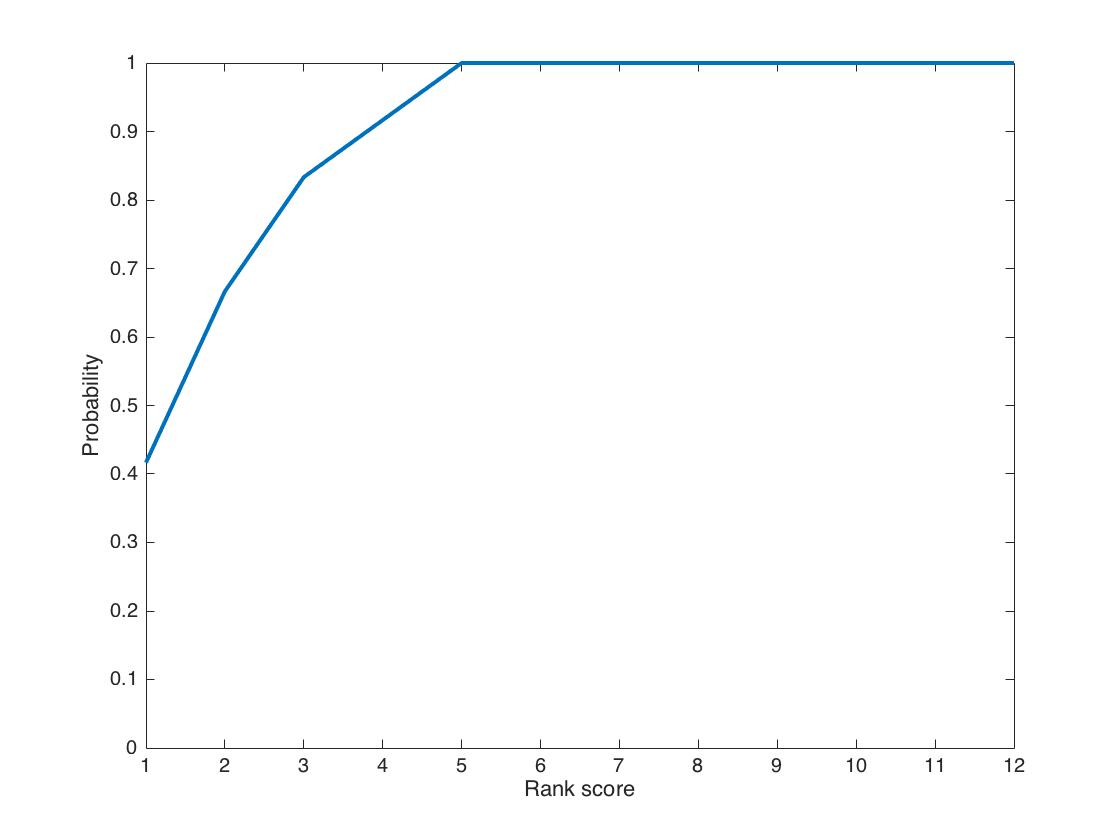
\includegraphics[width=1\linewidth]{/Users/JohnsonJohnson/Downloads/thesis_1/Figures/CMCexplanation.jpg}
\caption{A CMC plot of  gallery size is $M=10$ and probe size is $N=12$}
\label{CMCexplanationplot}
\vspace{-1em}
\end{figure} 






 
\chapter{Extraction of Hierarchical Gaussian descriptors}
In person re-identification, it is very important to choose robust descriptor to represent person. A good descriptor should be robust to variations of illumination, viewpoint, and camera color response. Most descriptors try to capture the color and texture information. In this chapter, we will first introduce some basic descriptors and compare their performance on VIPeR dataset, then a detailed introduction of a hierarchical descriptor will be presented in section 3.3 of this Chapter.


\section{Basic color and textural features}
\subsection{Color histogram descriptors on different color space}
Histogram descriptor extracts color statistics information of input images. A popular histogram extracting method is to divide input image into a few horizontal stripes and extract color histogram of each stripe, then they are concatenated to produce a histogram descriptor of the whole image. Color space selection has much influence on descriptor performance. HSV color space is commonly used in computer vision and image processing for target detection and tracking. The HSV descriptor has better performance than RGB histogram descriptor since HSV color separates image intensity from color information. Thus HSV color space is more robust to illumination variation. An unsupervised CMC performance comparison among different color spaces on VIPeR dataset is given in Figure \ref{CMCcolorspaces}. In this comparison camera A views are used as probe set and camera B views are used for gallery set. We can find that those color spaces separating intensity information outperform RGB color space by a large margin.
%-----------------------------------------------------------------------------

\begin{figure}[H]
\centering
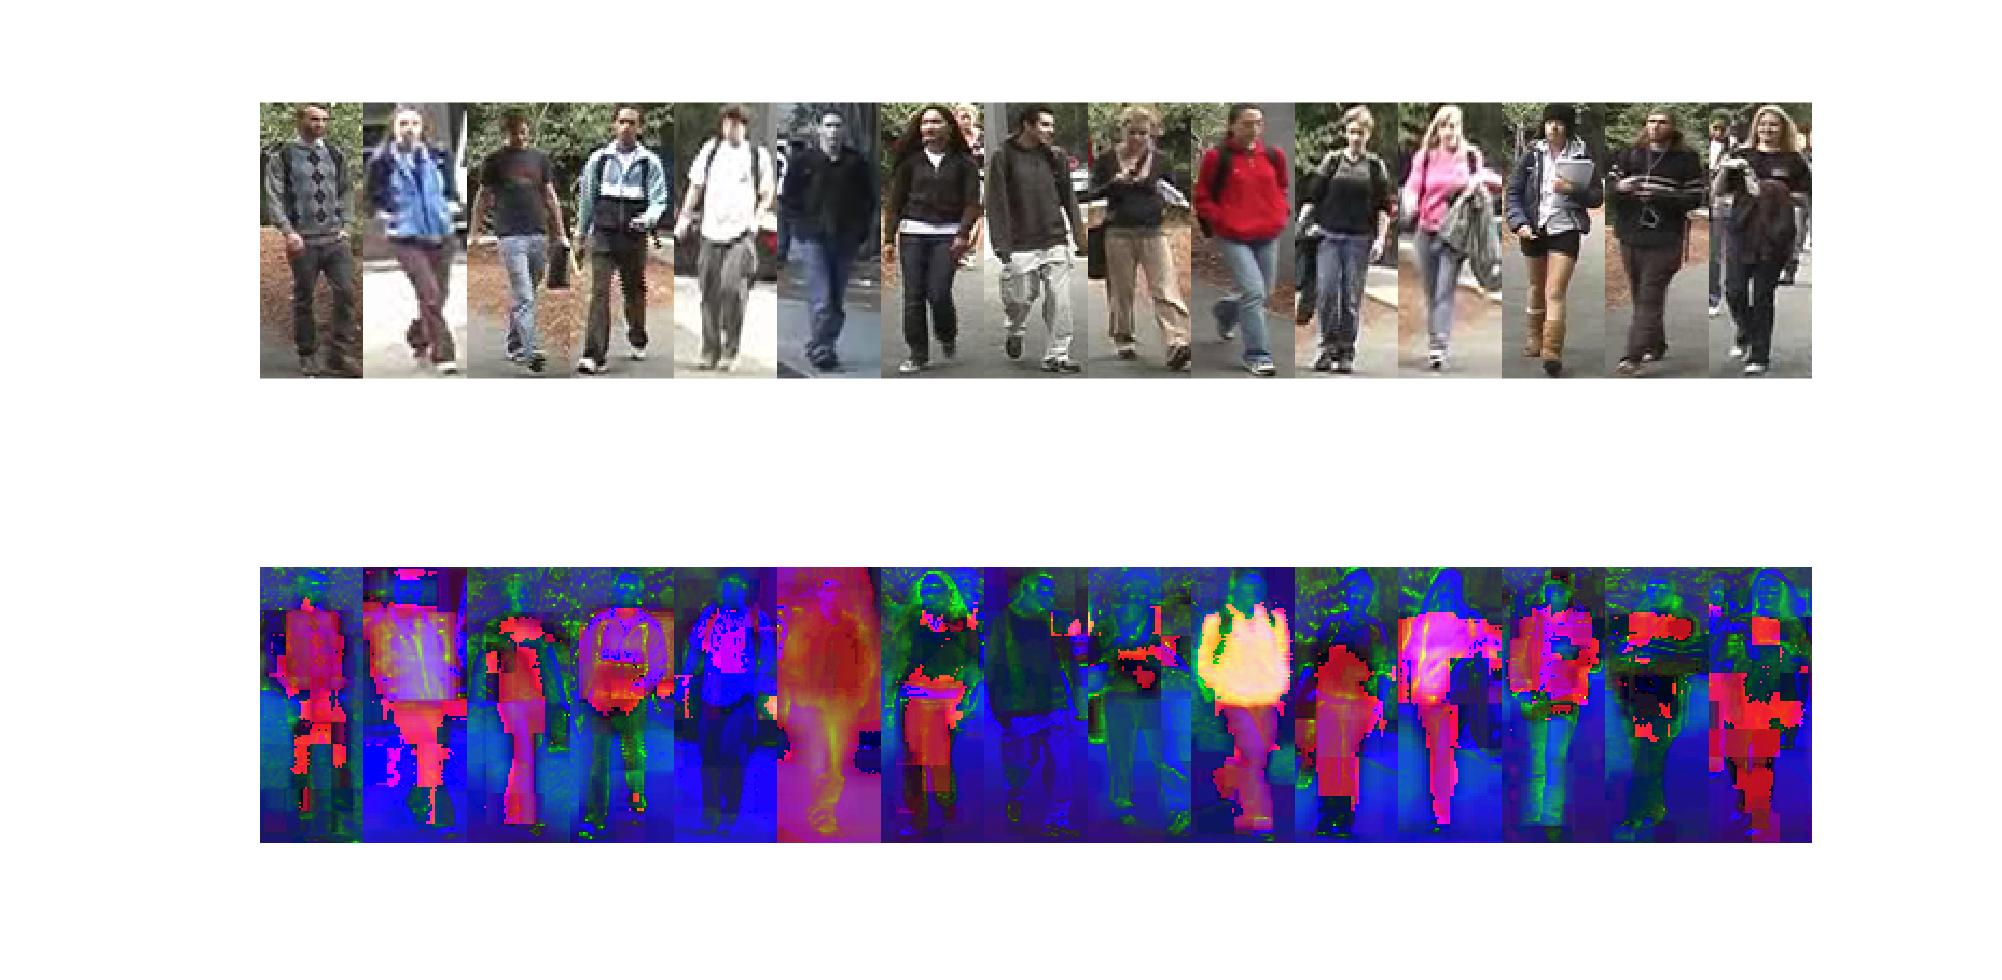
\includegraphics[width=1\linewidth]{/Users/JohnsonJohnson/Downloads/thesis_1/Figures/CompRGBHSV.jpg}
\caption{RGB and HSV visual comparison, the first row is RGB and second row is HSV for same views }
\vspace{0em}
\end{figure} 

\begin{figure}
\centering
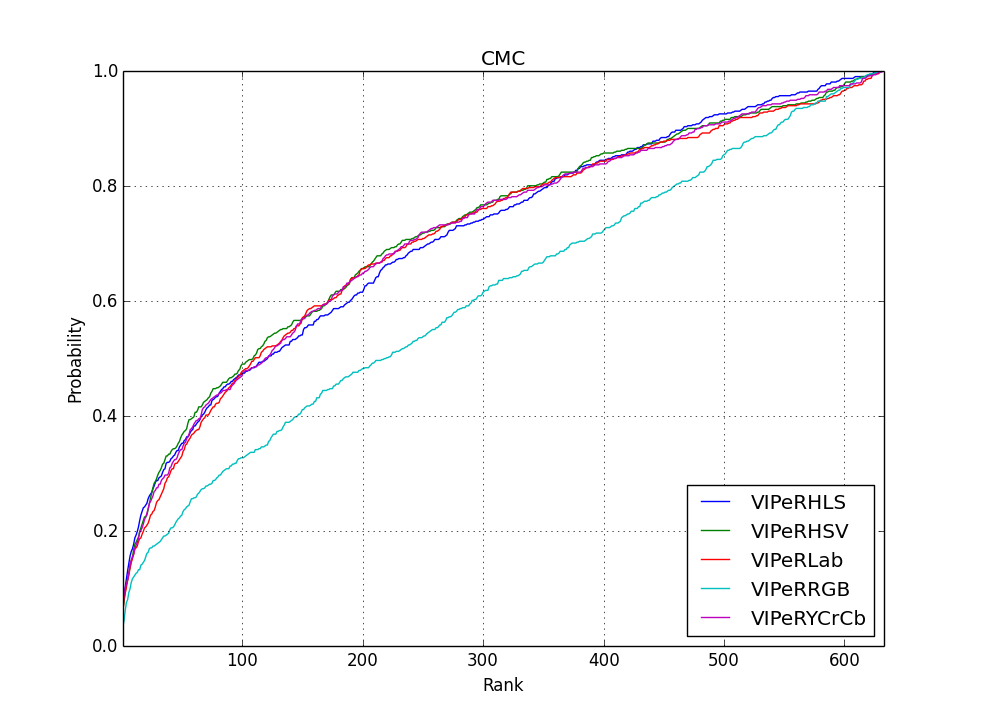
\includegraphics[width=1\linewidth]{/Users/JohnsonJohnson/Downloads/thesis_1/Figures/DifferentColorspaceCMCVIPeR.png}
\caption{A CMC comparison of color histogram on different color spaces }
\label{CMCcolorspaces}
\vspace{0em}
\end{figure} 

%-----------------------------------------------------------------------------

\textbf{Shortcoming of histogram based descriptor} The performance of histogram descriptors suffers from ignoring the spatial information. Since it doesn't consider the relative distribution of color patches. Images with same kind color patches but different distribution may have the same histogram descriptor. One example is shown in Figure \ref{RGBbgr}.

\begin{figure}[H]
\begin{minipage}[t]{0.5\linewidth}
\centering
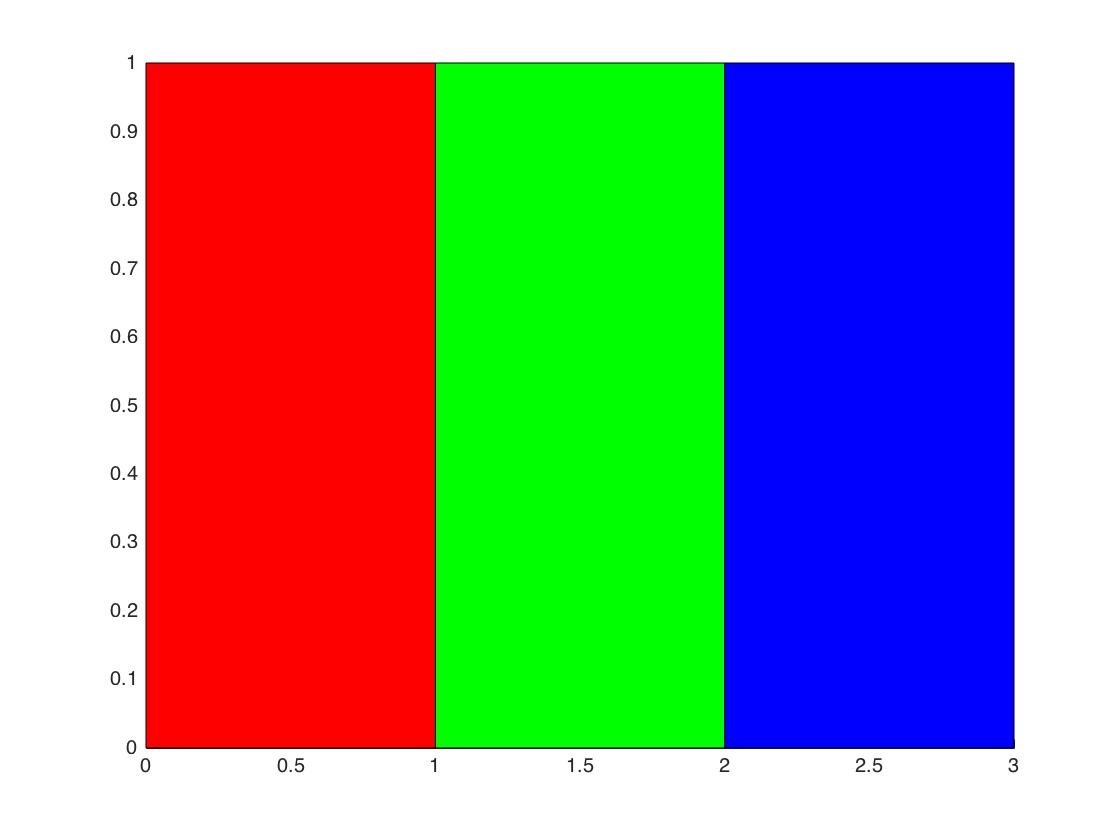
\includegraphics[width=2.2in]{/Users/JohnsonJohnson/Downloads/thesis_1/Figures/RGB.jpg}
%\caption{RGB patch}
\end{minipage}%
\begin{minipage}[t]{0.5\linewidth}
\centering
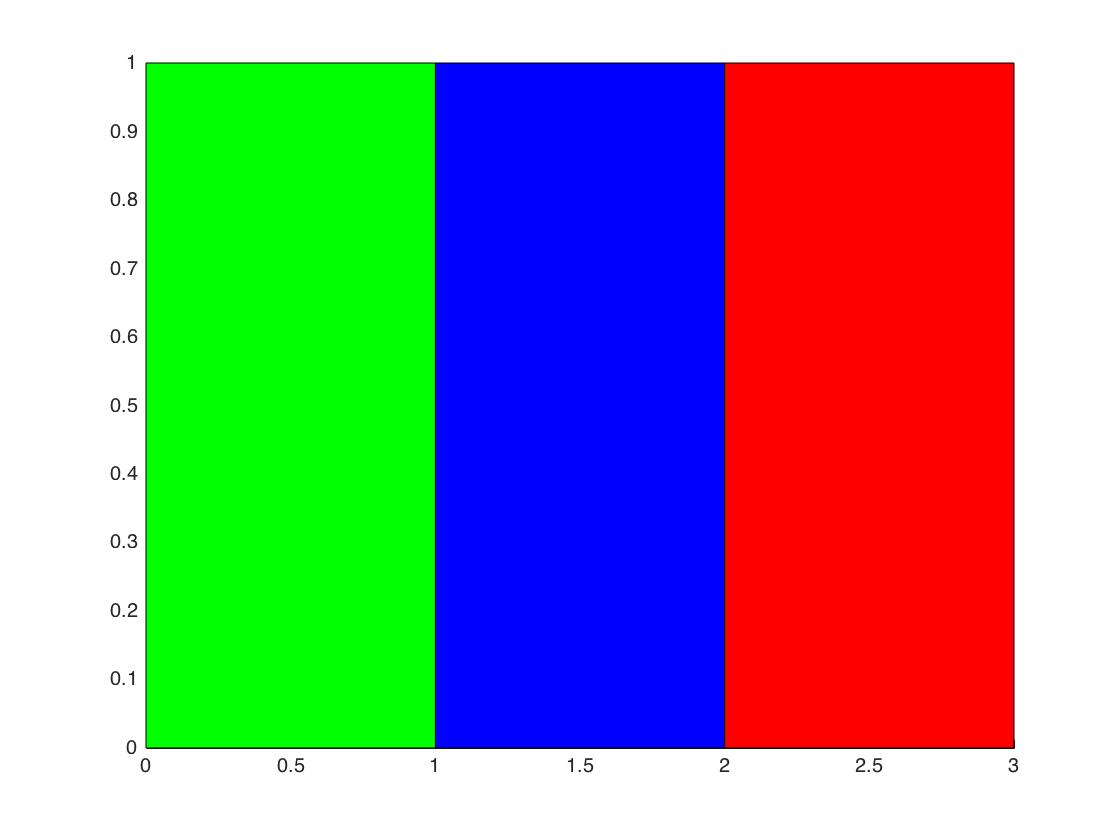
\includegraphics[width=2.2in]{/Users/JohnsonJohnson/Downloads/thesis_1/Figures/GBR.jpg}
%\caption{GBR patch}
\end{minipage}
\caption{A comparison of two patches with same entropy but different color distribution}
\label{RGBbgr}
\end{figure}


\subsection{Local binary pattern (LBP)}
Local binary pattern \cite{LBP1, LBP2} extracts the texture information with efficient computing and has been used on people detection and recognitions. Figure \ref{LBPdemoshot} is an example of LBP. by thresholding neighbour pixel of center pixel (shown in Figure \ref{LBPtheory}), the pixels are transformed into a binary integer. There are many extended LBPs like tLBP \cite{tLBP}, VLBP \cite{VLBP}, OCLBP \cite{OCLBP}. Besides, LBP is well known for its robustness to monotonic illumination variation.
\begin{figure}[H]
\centering
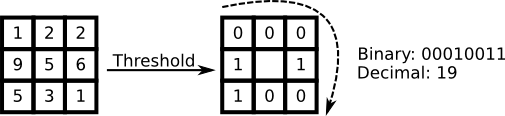
\includegraphics[width=0.8\linewidth]{/Users/JohnsonJohnson/Downloads/thesis_1/Figures/LBPdemo.png}
\caption{LBP: by thresholding the neighbour pixels the pixels are transformed into a binary number }
\label{LBPtheory}
\vspace{0em}
\end{figure}


\begin{figure}[H]
\begin{minipage}[t]{0.5\linewidth}
\centering
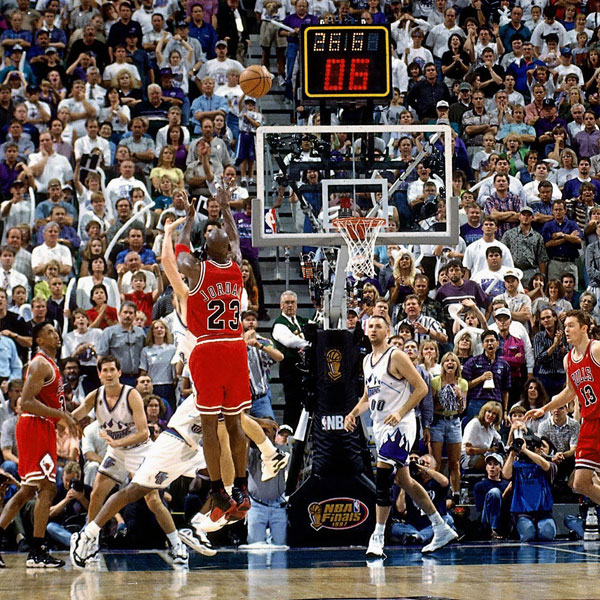
\includegraphics[width=2.2in]{/Users/JohnsonJohnson/Downloads/thesis_1/Figures/Theshot1.jpg}
\end{minipage}%
\begin{minipage}[t]{0.5\linewidth}
\centering
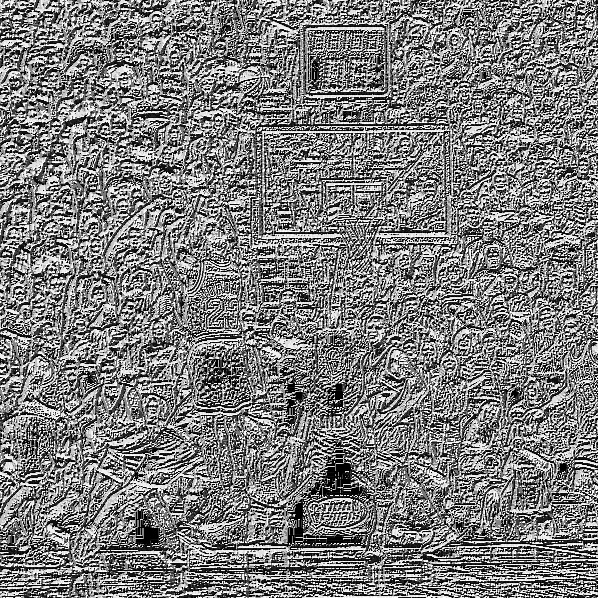
\includegraphics[width=2.2in]{/Users/JohnsonJohnson/Downloads/thesis_1/Figures/TheshotLBP1.jpg}
\end{minipage}
\caption{One LBP example}
\label{LBPdemoshot}
\end{figure}


\subsection{Histogram of oriented gradients (HOG)}
The HOG \cite{HOG} descriptor also extracts textural information of images by gradient computing. A brief introduction about its gradient computation is presented here, more details can be found in \cite{HOG}. HOG feature computes the gradient of input intensity  image $I(x, y)$ by equations 

\begin{equation}
\begin{aligned}
I_x = \frac{\partial I}{\partial x},\\
I_y = \frac{\partial I}{\partial y},
\end{aligned}
\end{equation}
the gradient can be computed fast by some discrete derivative masks below, like 1-D Sobel masks:
\begin{equation}
\begin{aligned}
Centered: M_{c} &= [-1, 0, 1]\\
Uncentered: M_{uc}& = [-1, 1]
\end{aligned}
\end{equation}
or 2-D Sobel masks:
\begin{equation}
\begin{aligned}
D_x = \left[ \begin{matrix}
0 & 1 \\
-1& 0
\end{matrix}
\right]\\
D_y = \left[ \begin{matrix}
-1 & 0 \\
0& 1
\end{matrix}
\right]
\end{aligned}
\end{equation}
or $3\times 3$ Sobel masks:
\begin{equation}
\begin{aligned}
S_x &= \left[ \begin{matrix}
-1 &0 & 1 \\
-2& 0 & 2\\
-1 &0 & 1 
\end{matrix}
\right]\\
S_y &= \left[ \begin{matrix}
1 & 2 &1 \\
0& 0 & 0\\
-1 & -2 &-1
\end{matrix}
\right]
\end{aligned}
\end{equation}

Using different masks will result different performance. Besides, gaussian smoothing is often performed before gradient computing. It has been shown that using 1-D Sobel without gaussian smoothing has the best performance. A HOG feature demo is shown in Figure \ref{fig:HOGdemo}.
\begin{figure}[H]
\centering
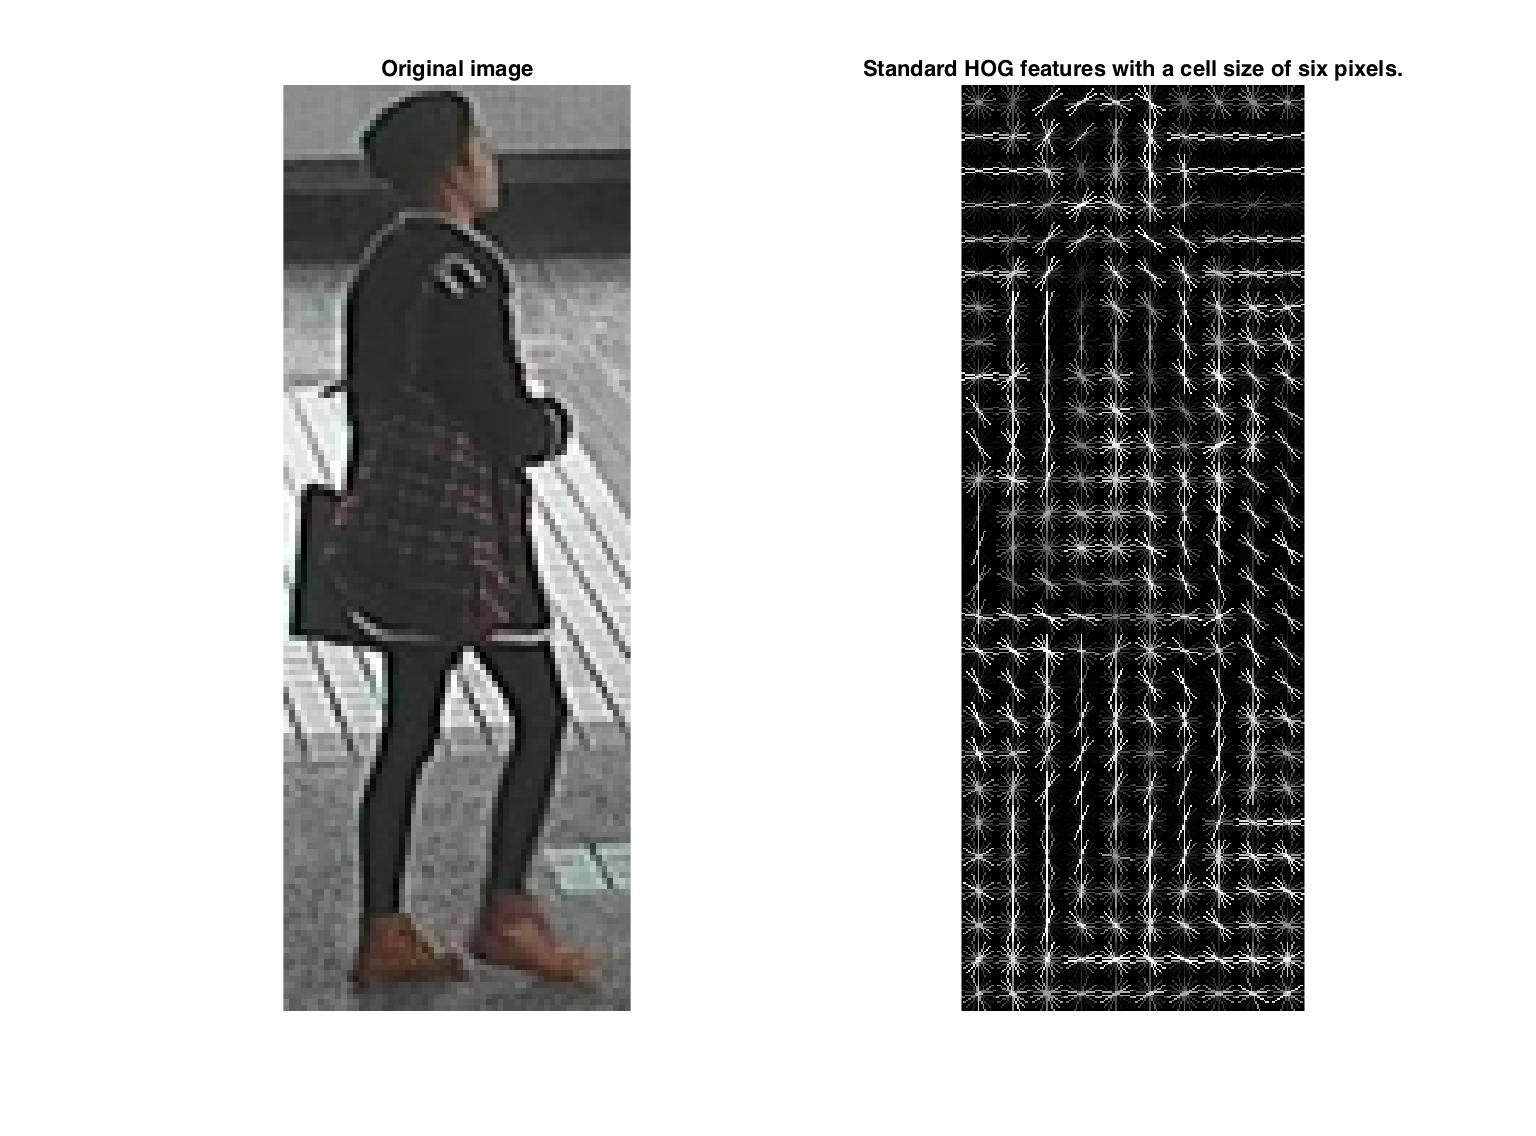
\includegraphics[width=1\linewidth]{/Users/JohnsonJohnson/Downloads/thesis_1/Figures/HOGfeatureDemo.jpg}
\caption{A demo of HOG feature with a cell size of six pixels}
\label{fig:HOGdemo} 
\vspace{0em}
\end{figure}


\section{Influence of background segmentation on different basic descriptors}
Many works try to minimize impact of background noise of pedestrians' image. It's easier to automatically segment foreground from a sequential frames or video than a single frame. In \cite{SDALF} the author provides foreground masks for all images following the algorithm in \cite{STEL}. Authors in \cite{STEL} propose stel (structure element) component analysis to model spatial correlations in image class structure by using probabilistic index maps (PIMs). A structure element is an area of an image with the same assigned index $s(s=1,2,\cdots,n)$, $n$ is the total number of stels in an image. In PIMs the indices assignment can be denoted probabilistically as a map $q(s_{\bm{i}}^s=s)$ over an image, in this equation the location is $\bm{i} = (i,j)$, $q$ is the probability of pixel at $\bm{i}$ of the $t$-th image (suppose there are many images for each class) belonging to the $s$-th stel. The authors propose that pixels in a structure element of an image class follow a shared distribution which can be modelled with local measurements like pixel intensity value. The number of stels $n$ is set to 2 to achieve background and foreground segmentation. That is, pixels of foreground stel share a distribution while pixels of background stel sharing another distribution. Both the foreground and background stels are modelled by a mixture of $C$ Gaussians. Some of those segmented foregrounds are shown in Figure \ref{VIPeRFGs} and it's obvious that certain body parts like head and feet are lost. To compare those loss impact on color and textural descriptors, a comparison of foreground segmentation on HSV color histogram descriptors, LBP and HOG descriptor is given in Figure \ref{fig:SegHSV}, Figure \ref{fig:SegLBP} and Figure \ref{fig:SegHOG}. 


\begin{figure}[H]
\centering
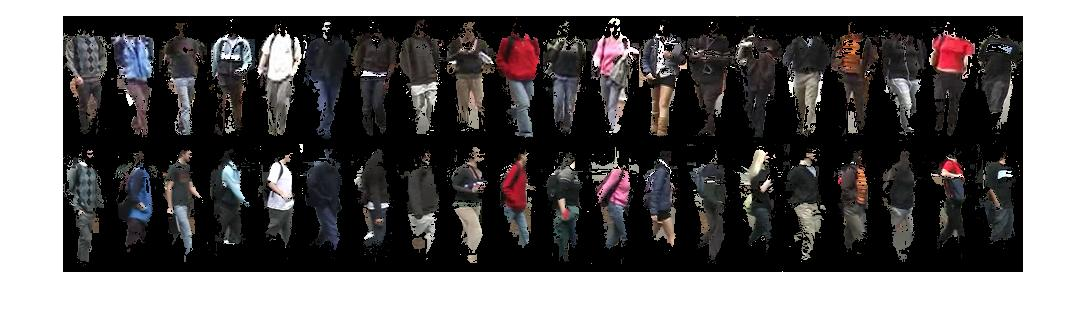
\includegraphics[width=1\linewidth]{/Users/JohnsonJohnson/Downloads/thesis_1/Figures/FGdemo2VIPeR.jpg}
\caption{Foreground segmentation of individuals from VIPeR }
\label{VIPeRFGs}
\vspace{0em}
\end{figure} 

We can find that foreground segmentation decreases LBP and HOG's performance but increases HSV color histogram's performance on VIPeR dataset greatly. The reason for this is imperfect foreground segmentation causes body parts (like head and feet) loss and mask out many parts in torso and legs. Besides, in images of some individuals, a part of background scene is regarded as foreground. Since HSV color histogram doesn't handle spatial distribution but only color entropy, foreground segmentation improves its performance greatly. But since LBP and HOG handle texture for each sample patch, their performance suffer from those body parts loss and little black patches from background. What's more, we can infer that imperfect foreground segmentation will also decrease other textural feature's performance.
\begin{figure}
\centering
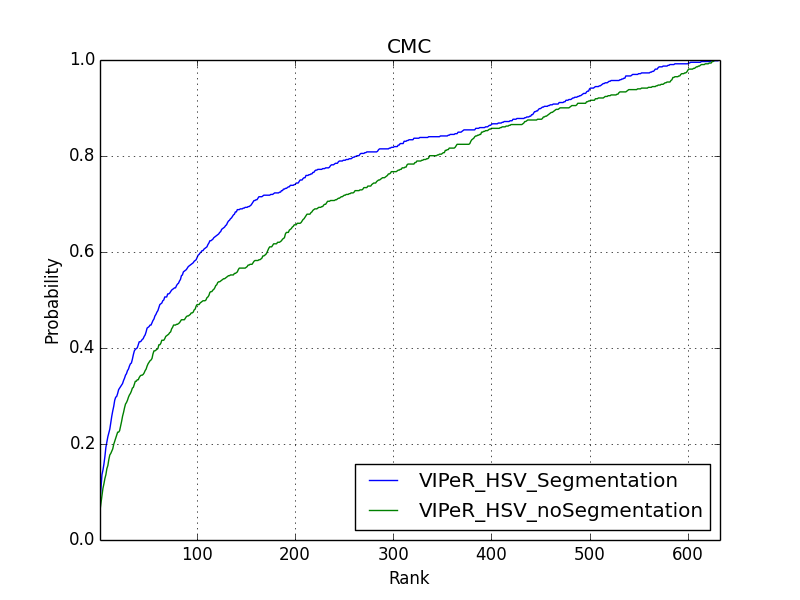
\includegraphics[width=1\linewidth]{/Users/JohnsonJohnson/Downloads/thesis_1/Figures/VIPeR_FG_HSV_comparison.png}
\caption{A CMC comparison of foreground segmentation on HSV histogram descriptor tested on VIPeR}
\label{fig:SegHSV}
\vspace{-1em}
\end{figure} 

\begin{figure}
\centering
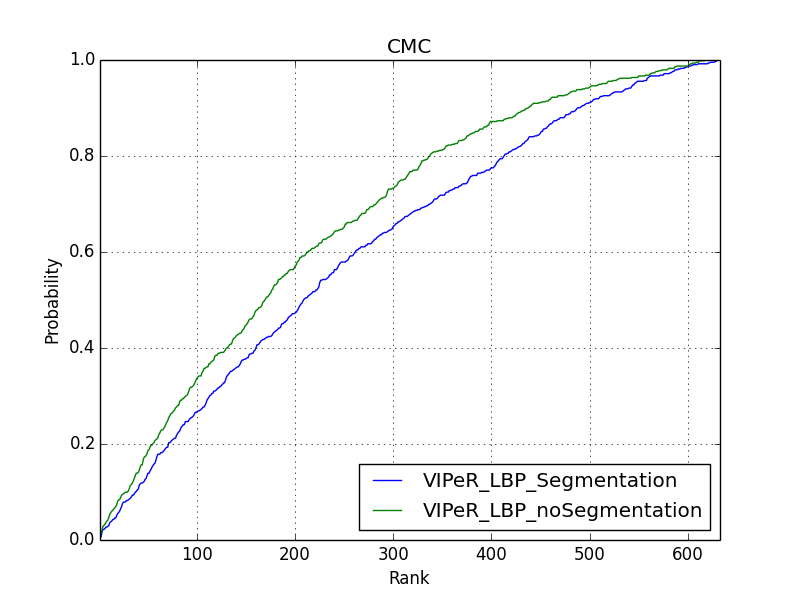
\includegraphics[width=1\linewidth]{/Users/JohnsonJohnson/Downloads/thesis_1/Figures/VIPeR_LBP_FGSegComparison.png}
\caption{A CMC comparison of foreground segmentation on LBP feature tested on VIPeR }
\label{fig:SegLBP}
\vspace{-1em}
\end{figure} 

\begin{figure}
\centering
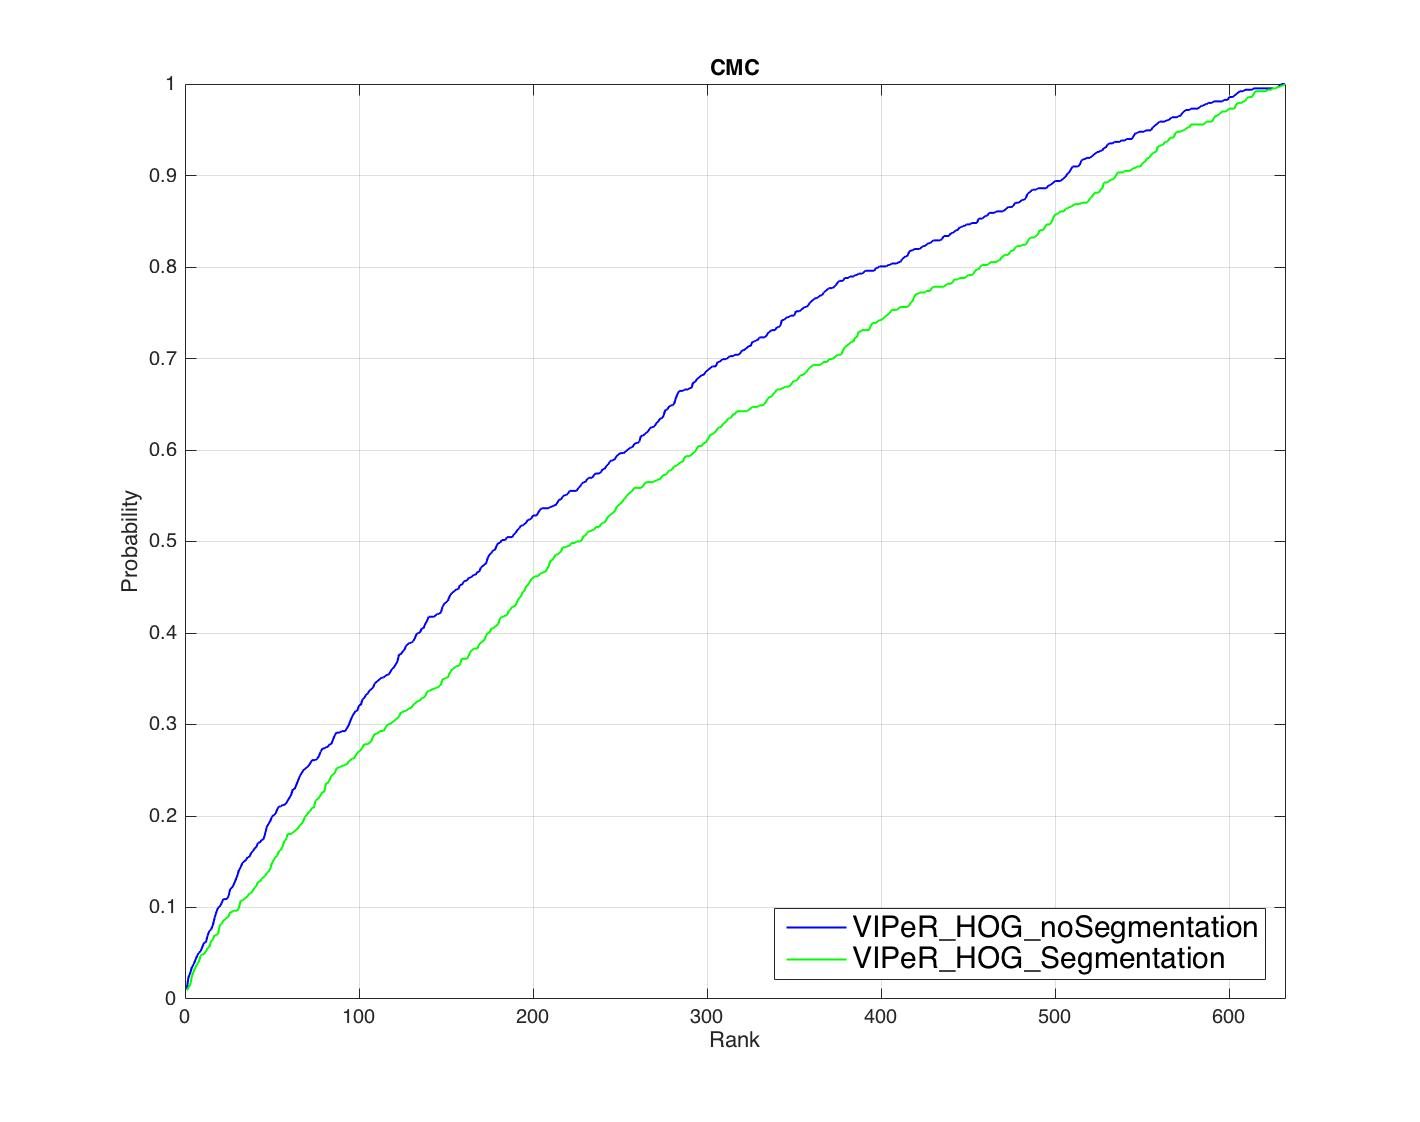
\includegraphics[width=1\linewidth]{/Users/JohnsonJohnson/Downloads/thesis_1/Figures/VIPeR_HOG_FGcomparison.jpg}
\caption{A CMC comparison of foreground segmentation on HOG feature tested on VIPeR}
\label{fig:SegHOG}
\vspace{-1em}
\end{figure} 

\section{The hierarchical gaussian descriptor}

The hierarchical gaussian descriptor is proposed by in  \cite{GOG}, this descriptor uses a two-level gaussian distribution to model an individual. This descriptor densely samples the image and models each hierarchical structure with gaussian distribution and to outperform many other works. In this thesis, all input images are sized to $128\times 64$. Firstly it divides the image into 7 overlapping horizontal slices, each slide has size $32\times 64$ and slides are overlapping by $16$ pixels vertically.  In each slide, densely sampled square patches have a size of $s\times s$ pixels ($s$ = 5 in this thesis), and small patches overlaps with each other by $2$ pixels. So there is a  two-level structure in this image, small patches and slides. The small patches are first modelled with a multivariate gaussian distribution, then with those small patch gaussian distributions, the slide containing those patches is modelled with another multivariate gaussian distribution.

In a certain horizontal slice for each small patch, it's modelled by a multivariate gaussian distribution $G_p(\bm{f}_i;\bm{\mu}_p,\bm{\Sigma}_p)$, and $G_p$ can be transformed to a vector $\bm{p}$ by SPD mapping. Again, when all small patches are modelled and vectorized, the same process is repeated. Each slide is characterized by a multivariate gaussian distribution $\bm{G}_r(\bm{p};\bm{\mu}_r,\bm{\Sigma}_r)$.\\
\indent After the slide is modelled with $\bm{G}_r(\bm{p};\bm{\mu}_r,\bm{\Sigma}_r)$, the same transformation will be operated on $\bm{G}_r$ so that it's vectorized as a vector $\bm{v}$. At last all computed $\bm{v}$ are concatenated to consist of the descriptor of current image. 

\subsection{Handling the background}
In the previous section the impact of background subtraction on different features' performance have been studied. We've concluded that imperfect foreground segmentation decreases textural feature's performance. Besides, in hierarchical gaussian descriptor there is no histogram-based feature computing. So in this thesis, when computing the pixel basic feature $\bm{f}_i$, the foreground segmentation is not adopted. But when modelling the region gaussian $\bm{G}_r(\bm{p};\bm{\mu}_r,\bm{\Sigma}_r)$ a weighted map is computed for each patch with equation
\begin{equation} 
N(x;\mu_0,\sigma_0) = \frac{1}{\sigma_0\sqrt{2\pi}} \exp^{\frac{(x - \mu_0)^2}{\sigma_0^2}}
\end{equation}
and here $\mu_0 = \frac{W_0}{2}, \sigma_0 = \frac{W_0}{4}$, $W_0$ is the number of patches in horizontal direction.
\subsection{Single pixel modelling}

In this hierarchical model, it is very important to have a full representation for every single pixel. To fully characterize single pixel, a $d$ dimensional vector is used to represent it. In this vector, there could be any predefined properties like coordinates, color values, texture and filter response. Suppose the original image is in RGB color space, the gaussian of gaussian descriptor uses a 8-dimensional vector $\bm{f}_i$, and 
$\bm{f}_i = (y,M_0,M_{90},M_{180},M_{270},R,G,B)$.
The y component is the y coordinate of pixel, and $M_{\{{\theta}\in{0^o,90^o,180^o,270^o}\}}$ is the quantized gradient information in 4 directions. The last three components are the color values of the specified color space.

In all the benchmark dataset, all the images are cropped with a bounding box, and the pedestrian in an image can be at left or right of center, while in the vertical direction the head and feet of pedestrian is very close the image edge. For each pixel, the y coordinate is more correlated than x coordinate, so only y coordinate is chosen for pixel modelling. 

Then the $M$ is to characterize the texture with the gradient histogram. Different $M$ values is the magnitude of gradient in every direction. 
Firstly the gradient in x and y direction are computed by two gradient filters $\rm{h}_x$ and $\rm{h}_y$, and we have 
\begin{equation}
\begin{aligned}
h_x &= [-1, 0, 1]\\
h_y &= -h_x'
\end{aligned}
\end{equation}

Then by convolving those two filters with the intensity image $I$, the horizontal and vertical gradient $I_x, I_y$ can be computed, so the orientation and magnitude can be computed by following equations:
\begin{equation}
\begin{aligned}
O(i,j) &= (\arctan(\frac{I_y(i,j)}{I_x(i,j)}+\pi)*180 /{\pi} \\
M(i,j) &= \sqrt{(I_x(i,j)^2 + I_y(i,j))^2}
\end{aligned}
\end{equation}

The orientation are quantized into four bins by a soft voting algorithm \cite{AutoRela}. For each pixel its corresponding gradient orientation is decided by its nearest bin's direction. To make the descriptor to focus on the gradient components with high values, the gradient and orientation are multiplied as follow,
\begin{equation}
M_{\theta} = MO_{\theta},
\end{equation}

%For every gradient magnitude value with its orientation , the corresponding weights of all predefined directions are computed, and the direction with the biggest weight is chosen as the quantized direction for this pixel.

To model the patch with a multi-variate gaussian distribution, we have to estimate its mean value and the covariance matrix. A multi-variate gaussian model has the form
\begin{equation}
G_p(\bm{f}_i;\bm{\mu}_p,\bm{\Sigma}_p) = \frac{\exp^{(\frac{1}{2}(\bm{f}_i-\bm{\mu}_p)^T\bm{\Sigma_p}^{-1}(\bm{f}_i-\bm{\mu}_p))}}{(2\pi)^{d/2}|{\bm{\Sigma}_p|}} 
\end{equation}
where $\bm {\mu}_p$ is the estimated mean value, and $\bm {\Sigma}_p $ is the estimated covariance matrix of current small patch. 

To estimate the parameters for this gaussian model based on sampled patches pixel features, the maximal likelihood estimate(MLE) is used. According MLE algorithm, we have the following estimated parameters
\begin{equation}
%\begin{aligned}
\bm{\mu}_p = \frac{1}{n}\sum_{i = 1}^n \bm{f}_i,
%\end{aligned}
\end{equation}
\begin{equation}
%\begin{aligned}
\bm{\Sigma}_p = \frac{1}{n-1} \sum_{i = 1}^n(\bm{f}_i-\bm{\mu})(\bm{f}_i-\bm{\mu})^T,
%\end{aligned}
\end{equation}

where $n$ is the number of pixels in current patch. When the gaussian model is computed, the next step is to model all the patch gaussians. But it's a complex problem to directly model those multivariate gaussian functions. So some transformation will be operated on the estimated parameters $\bm{\mu}_p$ and $\bm{\Sigma}_p$.


%% --------------------------------------Riemannian manifold based SPD transformation
\subsection{Riemannian manifold based SPD transformation}

As described before this hierarchical gaussian descriptor is a stochastic feature, so operations like computing mean and covariance need to be operated on previous summarized gaussian distributions. Mean and covariance operation in Euclidean space can not be directly finished on previous estimated gaussian functions. A transformation is needed to make stochastic summarization feasible on patch gaussian function.
In fact, the multivariate gaussian model is a Riemannian manifold and can be embedded into a semi-positive definite matrix (SPD) space. The gaussian function is mapped into a vector space by Equation \ref{SPDmapping}. A $d$ dimensional multivariate gaussian function can be mapped into a $d+1$ dimensional $SPD_+$ space. According to \cite{MultiVarGau}, the mapping can be denoted as 
\begin{equation}\label{SPDmapping}
G(\bm{x}_i;\bm{\mu}_i,\bm{\Sigma}_i) \sim \bm{P}_i  = |\bm{\Sigma}_i|^{1/(d+1)} \left[ \begin{matrix}
\bm{\Sigma}_i + \bm{\mu}_i\bm{\mu}^T & \bm{\mu}_i \\
\bm{\mu}_i^T & 1
\end{matrix}
\right]
\end{equation}
The covariance matrix $\bm{\Sigma}_i$ can be singular for small number of pixels within the patch, to avoid this problem a regular factor $\lambda$ is added to $\bm{\Sigma}_i$ so that $\bm{\Sigma}_i = \bm{\Sigma}_i + \lambda\bm{I}$. 

After this mapping, the $n+1$ dimensional SPD matrix needs to be transformed into a vector. The matrix logarithm is used to transform it to tangent space. A $d+1$ dimensional SPD matrix can be mapped as a $d*(d+3)/2+1$ vector, which can be denoted as $SPD_i^+ \sim \bm{p}_i = vec(log(\bm{P}_i))$. Since $\bm{P}_i$ is a positive symmetric matrix, it can be compressed by half, i.e only the upper triangular elements are preserved. To ensure its norm-1 remains the same after compression, the magnitude of off-diagonal elements in $\bm{P}_i$ are timed by $\sqrt2$.  Let $\bm{Q}=\log{\bm{P}_i}$, we have
\begin{equation}\label{vectorize}
%\begin{aligned}
 \bm{p}_i = [\bm{Q}_{1,1},\sqrt2\bm{Q}_{1,2},\sqrt2\bm{Q}_{1,3},\cdots,\sqrt2\bm{Q}_{1,d+1},
 \end{equation}
 \begin{equation}
 \bm{Q}_{2,2},\sqrt2\bm{Q}_{2,3,},\cdots,\sqrt2\bm{Q}_{2,d+1,},\cdots,\bm{Q}_{d+1,d+1,}]
%\end{aligned}
\end{equation}


Again we model the slide with a multivariate gaussian distribution $\bm{G}_r$ by equation
\begin{equation}
G_p(\bm{p}_j;\bm{\mu}_r,\bm{\Sigma}_r) = \frac{\exp^{(\frac{1}{2}(\bm{p}_j-\bm{\mu}_r)^T\bm{\Sigma_r}^{-1}(\bm{p}_j-\bm{\mu}_r))}}{(2\pi)^{d/2}|{\bm{\Sigma}_r|}} 
\end{equation}
we have known that all patches inside this slide been represented as vector $\bm{p}_j$, thus the mean $\bm{\mu}_r$ and covariance matrix ${\bm{\Sigma}}_r$ of $\bm{G}_r$ can be computed by MLE with equations
\begin{equation}
%\begin{aligned}
\bm{\mu}_r = \frac{1}{m}\sum_{j = 1}^m \bm{p}_j,
%\end{aligned}
\end{equation}
\begin{equation}
%\begin{aligned}
\bm{\Sigma}_r = \frac{1}{m -1} \sum_{j = 1}^m(\bm{p}_j-\bm{\mu}_r)(\bm{p}_j-\bm{\mu}_r)^T,
%\end{aligned}
\end{equation}
m is the total number pf patches inside current slide. Again $\bm{\mu}_r$ and $\bm{\Sigma}_r$ are mapped to a SPD space by equation
\begin{equation}
G(\bm{p};\bm{\mu}_r,\bm{\Sigma}_r) \sim \bm{P}_r  = |\bm{\Sigma}_r|^{1/(d+1)} \left[ \begin{matrix}
\bm{\Sigma}_r + \bm{\mu}_r\bm{\mu}_r^T & \bm{\mu}_r \\
\bm{\mu}_r^T & 1
\end{matrix}
\right]
\end{equation}
and $\bm{P}_r$ is vectorized by Equation \ref{vectorize}.

When all horizontal slides' descriptor computed they are concatenated to form the descriptor for the whole image.



%%Integral image for fast computing
\subsection{Integral image for fast region covariance computation}

To compute estimated parameters for all those overlapping small patches, the time complexity of computing one by one each patch is high because there are many repeating computations. To compute the estimated covariance matrix \bm{$\Sigma}$ for every small patch with size of $W\times H$, the integral image is used to reduce time complexity. The integral image \cite{RegionCovariance} is a intermediate representation to fast compute rectangle area sum in an image. Each pixel value in integral image is the sum of all the pixels inside the rectangle bounded by current pixel and the upper left pixel. That is, the integral image S(x, y) for image I(x, y) is 
\begin{equation}
S(x', y') = \sum_{x<x', y <y'} I(x, y),
\end{equation}

\begin{figure}[H]
\centering
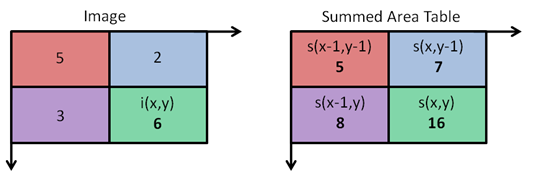
\includegraphics[width=1\linewidth]{/Users/JohnsonJohnson/Downloads/thesis_1/Figures/IntegralImage.png}
\caption{Integral image}
\vspace{0em}
\end{figure} 
By using integral image any rectangular region sum can be computed in constant time. \\
\indent To compute the covariance matrix of a certain rectangle area in a $W\times H\times d$ dimensional feature tensor $F$, suppose $\bm{I}_F$ is the $W\times H\times d$ tensor of integral images of $F$, we have 
\begin{equation}
 \bm{I}_F(x', y', i) = \sum_{x < x', y < y'}F(x, y ,i), i = 1 \dots d
\end{equation} 
and suppose the $\bm{C}(x', y', i, j)$ is the $W\times H\times d\times d$ tensor of second order integral images, we have
\begin{equation}
\bm{C}(x', y', i, j) = \sum_{x<x', y<y'} F(x, y, i)F(x, y, j), i, j = 1 \dots d.
\end{equation}
let $\bm{I}_{x, y}$ be the $d$ dimensional vector in $\bm{I}_F$, $\bm{C}(x, y)$ be the $d\times d$ dimensional matrix in $\bm{C}$, 
\begin{equation}
\begin{aligned}
\bm{I}_{x, y} = [ \bm{I}_F(x', y', 1) \dots  \bm{I}_F(x', y', d)]^T \\
 \bm{C}_{x, y} = \left [
 \begin{matrix} 
 \bm{C}(x, y, i, 1)  &\cdots & \bm{C}(x, y, 1, d)\\
 			     & \ddots &			        \\
\bm{C}(x, y, d, 1)   & \cdots &\bm{C}(x, y, d, d)
 
 \end{matrix} \right ]
 \end{aligned}
\end{equation}

Then for any rectangule regions $R(x', y'; x'', y'')$, where $(x', y')$ is the upper left coordinate and $(x'', y'')$ is the lower right coordinate, the covariance matrix can be compute as 
\begin{equation}
\begin{aligned}
\bm{C}_R(x', y'; x'', y'') = \frac{1}{n-1} [\bm{C}_{x'', y''} + \bm{C}_{x', y'} -  \bm{C}_{x'', y'}-  \bm{C}_{x', y''} \\
-\frac{1}{n}(\bm{I}_{x'', y''} + \bm{I}_{x'', y''} - \bm{I}_{x', y''} - \bm{I}_{x'', y'})(\bm{I}_{x'', y''} + \bm{I}_{x'', y''} - \bm{I}_{x', y''} - \bm{I}_{x'', y'})^T]
\end{aligned}
\end{equation}
where $n$ is the number of feature vector in $F$, and $n = (x'' - x')(y'' - y')$. By creating the integral image the covariance of any rectangular area in $F$ can be computed in $O(d^2)$ time.

When all patches in a region are computed, the same process is repeated to compute the region gaussian. 


\subsection{Dimensionality and superiority analysis of Hierarchical Gaussian descriptor}
It has been known that combination of descriptors of different color space can greatly improve re-ID performance. In this project, the hierarchical gaussian descriptor in RGB color space is the base descriptor. Descriptors in three more color space \{HSV, Lab, nRGB\} are extracted. The nRGB color space is calculated as 
\begin{equation}
\begin{aligned}
nR = \frac{R}{R+G+B},\\
nG = \frac{G}{R+G+B},\\
nR = \frac{B}{R+G+B}, 
\end{aligned}
\end{equation}
since $nB$ can be calculated with $nR$ and $nG$, in this color space only the first two channel values are used to reduce redundancy. Therefore, for color space \{RGB, HSV, Lab, nRGB\}, the corresponding dimension of pixel feature is \{8, 8, 8, 7\}. After the matrix to vector transformation, the dimension of patch gaussian vector of each channel is \{45, 45, 45, 36\}. Again after the patch gaussian to region gaussian transformation, the dimension of each channel is \{1081, 1081, 1081, 703\}. Suppose there are 7 horizontal slides in each image, the dimension of concatenated descriptor of each channel is \{7567, 7567, 7567, 4921\}. If four color space are all used, the dimension is the sum of each channel as 27622. 

Hierarchical gaussian descriptor has a few advantages compared with other descriptors. Firstly, it has a full consideration of color, texture and $y$ coordinate information. The color information is adopted by adding color values of different color space to $\bm{f}_i$. Textural information is also adopted by those four gradient components in $\bm{f}_i$. Secondly, by Riemannian manifold based SPD mapping, it provides a solution to summarize many multi-variate gaussian functions. The parameters $\bm{\mu}$ and $\bm{\Sigma}$ of a multi-variate gaussian function can be fused into a SPD matrix. With later vectorization this SPD matrix is transformed to a vector. In this mapping process correlation of different components in $\bm{f}_i$ are fully taken into account, which leads to a dimension increasing from basic pixel feature vector $\bm{f}_i$ to patch gaussian vector $\bm{p}_j$. Thirdly, by a two-level gaussian model, this model guarantees to extract the overall statistical information of an image while being robust to local details variation caused by factors like viewpoint changes and partial occlusion. 

It is intractable to directly learn a Mahanalobis distance matrix from concatenated Hierarchical Gaussian descriptor. In next Chapter KLFDA is applied to reduce the dimensionality of extracted descriptor from 27622 to $n-1$, where $n$ is the number of different classes. With this supervised nonlinear dimensionality reduction, discriminative information among different classes are preserved. At last a Mahanalobis matrix is learned on the dimension reduced descriptors by gradient descent method.




%\section{Kernel fisher discriminant analysis}
%The extracted hierarchical gaussian descriptors have high dimension, it's intractable to learn a SPD matrix with such a high dimension. Dimension reduction is required to learn a subspace.
%Among those methods to reduce dimension, principal component analysis (PCA) is often used. However, PCA is an unsupervised dimension reduction and may have a low performance for those reasons, $(1)$, PCA is to maximize the variance of dimension reduced data, and as a unsupervised method it doesn't has a full consideration of the the relation of between and within classes, it is very likely that the descriptors of different classes can be mixed up after the dimension reduction; $(2)$ PCA may suffer from the small sample size problem. In some Re-ID datasets, there may be two or less images for each pedestrian in each viewpoint (like VIPeR), if the dimension of descriptor is much bigger than sample size, much information can be lost with PCA. In this thesis, the kernel local fisher discriminant analysis (KLFDA) is used to reduce dimension. 
%\subsection{Fisher discriminant analysis (FDA)}
%KLFDA is the kernel version of LFDA, and LFDA is a combination of Fisher discriminant analysis[ ] and and the locality preserving projection in [LPP ] and kernel method. A brief introduction of FDA, LPP and kernel method is introduced below.
%
%FDA is a supervised dimension reduction and its input contains the class labels. For a set of $d$-dimensional observations $\bm{x}_i$, where $i\in\{1,2,\cdots,n\}$, the label $l_i\in\{1,2,\cdots,l\}$. Two matrix are defined as the intraclass scatter matrix $\bm{S}^{(w)}$ and between class scatter matrix
%$\bm{S}^{(b)}$, 
%\begin{equation}
%\begin{aligned}
%\bm{S}^{(w)} &= \mathop{\sum} _{i=1}^l\mathop{\sum}_{j:l_j = i} (\bm{x}_j - \bm{\mu}_i)(\bm{x}_j - \bm{\mu}_i)^T \\
%\bm{S}^{(b)}  &= \mathop{\sum} _{i=1}^l n_i(\bm{\mu}_i - \bm{\mu})(\bm{\mu}_i - \bm{\mu})^T
%\end{aligned}
%\end{equation}
%where the $\bm{\mu}_i$ is the mean of samples whose label is $i$, and $\bm{\mu}$ is the mean of all samples,
%\begin{equation}
%\begin{aligned}
%\bm{\mu}_i &= \frac{1}{n_i} \sum \bm{x}_i, \\
%\bm{\mu} &= \frac{1}{n} \sum \bm{x}_i
%\end{aligned}
%\end{equation}
%
%The Fisher Discriminant Analysis transform matrix $\bm{T}$ can be represented as 
%\begin{equation}
%\bm{T} = \arg\max \frac{\bm{T}^T\bm{S}^{(b)}\bm{T}}{\bm{T}^T\bm{S}^{(w)}\bm{T}}
%\end{equation}
%This equation can be solved by Lagrange multiplier method, we define a Lagrange function 
%\begin{equation}
%L(\bm{t}) = \bm{t}^T\bm{S}^{(b)}\bm{t} - \lambda(\bm{t}^T\bm{S}^{(w)}\bm{t} - 1)
%\end{equation}
%Then the differential respect to $\bm{t}$ is 
%\begin{equation}
%\frac{\partial L(\bm{t})}{\partial \bm{t}} = 2\bm{S}^{(b)}\bm{t} - 2\lambda \bm{S}^{(w)}\bm{t}
%\end{equation}
%
%let 
%\begin{equation}
%\frac{\partial L(\bm{t})}{\partial \bm{t}} = 0
%\end{equation}
%
%we can get 
%\begin{equation}
%\bm{S}^{(b)}\bm{t}_i  = \lambda \bm{S}^{(w)}\bm{t}_i
%\end{equation}
%\label{eigen1}
%
%here $\bm{t}_i$ is the $i_{th}$ column of $\bm{T}$, and the optimization problem is converted to a eigenvalue decomposition problem. 
%
%Fisher discriminant analysis tries to minimize the intraclass scatter matrix while maximize the interclass scatter matrix, and $\bm{T}$ is computed by the eigenvalue decomposition. $\bm{T}$ can be represented as the set of all the corresponding eigenvectors, as $ \bm{T} = (\bm{t}_1,\bm{t}_2,\cdots,\bm{t}_k)$.
%
%FDA has a form similar with signal and noise ratio, however, the FDA dimension reduction may have poor performance for it doesn't consider the locality of data. An example of this is the multimodality[]. Multimodality is the case many clusters are formed in the same class. 
%\subsection{Locality preserving projection (LPP)}
%
%In \cite{LPP} locality preserving projection (LPP) is proposed to exploit data locality. An affinity matrix is created to record the affinity of sample $\bm{x}_i$ and $\bm{x}_j$,  typically the range of elements in $\bm{A}_{i,j}$ is $[0,1]$. There are many manners to define a $n \times n$ affinity matrix $\bm{A}$, usually two sample points with a smaller distance has a higher affinity value than those with bigger distance value. One of them is if  $\bm{x}_i$ is within k-nearest neighbours of $\bm{x}_j$ then $\bm{A}_{i,j} = 1$ otherwise  $\bm{A}_{i,j} = 0$.  
%
%Another diagonal matrix $D$ can be defined that each diagonal element is the sum of corresponding column in $\bm{A}$,
%\begin{equation}
%\bm{D}_{i,i} = \mathop{\sum}_{j=1}^n \bm{A}_{i, j} 
%\end{equation}
%then the LPP transform matrix is defined as follow,
%\begin{equation}
%\bm{T}_{LPP} = \mathop{\arg\min}_{\bm{T}\in\bm{R}^{d\times m}} \frac{1}{2}\mathop{\sum}_{i, j= 1}^n \bm{A}_{i,j} ||\bm{T}^T\bm{x}_i - \bm{T}^T\bm{x}_j||
%\end{equation}
%so that $ \bm{T}^T\bm{X}\bm{D}\bm{X}^T\bm{T} = \bm{I} $.
%Suppose the subspace has a dimension of $m$, then LPP transform matrix $T$ can be represented as 
%
%$$\bm{T}_{LPP} = \{ \bm{\phi}_{d-m+1} | \bm{\phi}_{d-m+2} | \cdots \bm{\phi}_{d}\} $$
%
%And each $\bm{\phi}$ in $T$ is the eigenvector of following fomula,
% \begin{equation}
%\bm{X}\bm{L}\bm{X}^T\bm{\phi} = \gamma\bm{X}\bm{D}\bm{X}^T
%\end{equation}
%where $\gamma$ is corresponding eigenvalue of $\bm{\phi}$, and $L = D - A$.\\
%%But the LPP dimension reduction is still not discriminant enough, 
%\subsection{Local fisher discriminant analysis}
%\indent LFDA \cite{LFDA} combines FDA and LPP and have better performance. The key in LFDA is it assigns weights to elements in $\bm{A}^{(w)}$ and $\bm{A}^{(b)}$, so that,
%\begin{equation}
%\begin{aligned}
%\bm{S}^{(w)} &= \frac{1}{2}\sum _{i=1}^l\sum_{j:l_j = i} \bm{A}_{i,j}^w (\bm{x}_j - \bm{\mu}_i)(\bm{x}_j - \bm{\mu}_i)^T \\
%\bm{S}^{(b)} &=  \frac{1}{2}\sum _{i=1}^l \bm{A}_{i,j}^b(\bm{\mu}_i - \bm{\mu})(\bm{\mu}_i - \bm{\mu})^T
%\end{aligned}
%\end{equation}
%where 
%
%\begin{equation}
%\begin{aligned}
%\bm{A}_{i,j}^{(w)} = \left \{ 
%\begin{array}{rcl}
%\bm{A}_{i,j}/n_c &  &y_i = y_j \\
%0 & & else
%\end{array}
%  \right.  \\
%  \bm{A}_{i,j}^{(b)} = \left \{ 
%\begin{array}{rcl}
%(\frac{1}{n} - \frac{1}{n_c})  \bm{A}_{i,j} &  &{y_i = y_j }\\
%\frac{1}{n} & & {else}
%\end{array}
%  \right. 
% \end{aligned}
%\end{equation}
%where $y_i$ is the class label of sample point $\bm{x}_i$. So the transformation matrix $T_LFDA$ can be computed by equation
%\begin{equation}
%\bm{T}_{LFDA}  = \arg\min_{\bm{T}} (\frac{\bm{T}^T\bm{S}^{(b)}\bm{T}}{\bm{T}^T\bm{S}^{(w)}\bm{T}})
%\end{equation}
%\label{eigencompute1} 
%Again this problem can be solved by eigenvalue decomposition by equation \ref{eigen1}. 
%
%
%
%When applying the LFDA to original high dimensional descriptors, one problem is the computation cost. Suppose the vector data has a dimension of $d$, LFDA has to solve the eigenvalue a matrix with dimension $d\times d$. In some descriptors the $d$ could be more than 20000 and thus the computation cost is intractable. 
% 
%\subsection{Kernel local fisher discriminant analysis(KLFDA)}
%
%KLFDA  \cite{KLFDA} is the nonlinear version of LFDA. Most dimensionality reduction methods including PCA, LDA and LFDA are linear dimensionality reduction methods. However, when descriptors data are non-linear in feature space, its hard to capture its between-class discriminant information with linear reduction methods. One alternative method is to nonlinearly map input descriptors $\bm{x}_i$ to higher dimensional feature space $\Phi$ by a function $\phi(\bm{x}_i)$, again the LFDA is performed in feature space $\Phi$. Thus the transformation matrix $T$ can be computed by equation
%\begin{equation}
%\bm{T} = \arg \min \frac{\bm{T}^T\bm{S}^{(b)}_{\phi}\bm{T}}{\bm{T}^T\bm{S}^{(w)}_{\phi}\bm{T}}
%\end{equation}
%where $\bm{S}^{(b)}_{\phi}$ and $\bm{S}^{(w)}_{\phi}$ is the between class scatter and within class scatter in mapped feature space $\Phi$.
%
%Note that the transformation matrix $\bm{T} \in \Phi$, it's computationally expensive to explicitly compute the mapping function $\phi$ and perform LFDA in feature space $\Phi$ because the dimension of $\Phi$ may be infinite. Rather than explicitly computing, the mapping function $\phi$ can be implicit and the feature space $\Phi$ can be defined by the inner product of features in $\Phi$. Kernel trick [] is used here and a kernel function can be defined as the inner product of mapped vectors $\phi(\bm{x}_i)$ and $\phi(\bm{x}_j)$ by equation
% \begin{equation}
% k(\bm{x}_i,\bm{x}_j) = <\phi(\bm{x}_i),\phi(\bm{x}_j)>,
% \end{equation}
% the $< \cdot >$ is the inner product. There are many kinds of kernel like linear kernel, polynomial kernel and radial basis function (RBF) kernel. In this paper the RBF kernel is adopted. A RBF kernel is defined as 
% \begin{equation}
% k_{RBF}(\bm{x}_i,\bm{x}_j) = \exp^{(-\gamma||\bm{x}_i-\bm{x}_j||^2)}. 
% \end{equation}
%Suppose $\bm{X}$ is the sample descriptors matrix, and we have
%\begin{equation}
%\bm{X} = (\bm{x}_1, \bm{x}_2,\cdots, \bm{x}_n), 
%\end{equation}
%and the label vector is $\bm{l} = (l_1, l_2, \cdots, l_n)$. Then the kernel matrix of $\bm{X}$ can be computed as following equation:
%\begin{equation}
%\bm{K} =  \phi(\bm{X})^T \phi(\bm{X})
%\end{equation}
%and we have 
%\begin{equation}
%\bm{K}_{i,j} =  k(\bm{x}_i,\bm{x}_j) = <\phi(\bm{x}_i),\phi(\bm{x}_j)> =  \exp^{(-\gamma||\bm{x}_i-\bm{x}_j||^2)}
%\end{equation}
%
%In \cite{LFDAdr} the authors proposed fast computation of LFDA by replacing $\bm{S}^{(b)}$ with the local scatter mixture matrix $\bm{S}^{(m)}$defined by 
%\begin{equation}
%\begin{aligned}
%\bm{S}^{(m)} &= \bm{S}^{(b)} + \bm{S}^{(w)}\\
%\bm{S}^{(m)} &= \frac{1}{2} \sum_{i,j = 1} \bm{A}_{i,j}^{(m)} (\bm{x}_i - (\bm{x}_j)(\bm{x}_i - (\bm{x}_j)^T
%\end{aligned}
%\end{equation}
%and 
%
%\begin{equation}
%\bm{A}_{i,j}^{(m)} = \bm{A}_{i,j}^{(w)}  + \bm{A}_{i,j}^{(w)}
%\end{equation}
%
%\noindent according to indentify(Fukunaga, 1990)
%\begin{equation}
%tr((\bm{T}^T\bm{S}^{(w)}\bm{T})^{(-1)}(\bm{T}^T\bm{S}^{(m)}\bm{T}) = tr((\bm{T}^T\bm{S}^{(w)}\bm{T})^{(-1)}(\bm{T}^T\bm{S}^{(b)}\bm{T}) + m
%\end{equation}
%equation \ref{eigencompute1} is equal to 
%
%\begin{equation}
%\bm{T}_{LFDA}  = \arg\min_{\bm{T}} (\frac{\bm{T}^T\bm{S}^{(m)}\bm{T}}{\bm{T}^T\bm{S}^{(w)}\bm{T}})
%\end{equation}
%and it can be transformed into a eigenvalue decomposition problem 
%\begin{equation}
%\bm{S}^{(m)}\bm{t}_i  = \lambda \bm{S}^{(w)}\bm{t}_i
%\end{equation}
%\label{eigen2}
%Also with the replacement of $\bm{S}^{(m)}$, in \cite{LFDAdr} the author summarized that 
%\begin{equation}
%\bm{S}^{(m)} = \bm{X}\bm{L}^{(m)}\bm{X}^T
%\end{equation}
%where $\bm{L}^{(m)}  = \bm{D}^{(m)} - \bm{A}^{(m)}$, and $ \bm{D}^{i,i} = \sum_{j=1}^n  \bm{A}^{(m)}$. Also $\bm{S}^{(w)}$ can be represented as 
%\begin{equation}
%\bm{S}^{(w)} = \bm{X}\bm{L}^{(w)}\bm{X}^T
%\end{equation}
%where $\bm{L}^{(w)}  = \bm{D}^{(w)} - \bm{A}^{(m)}$, and $ \bm{D}^{i,i} = \sum_{j=1}^n  \bm{A}^{(w)}$. 
%Therefore, equation \ref{eigen2} can be represented as
%\begin{equation}
%\bm{X}\bm{L}^{(m)}\bm{X}^T \bm{t}_i= \lambda\bm{X}\bm{L}^{(w)}\bm{X}^T \bm{t}_i
%\end{equation}
%\label{equationS}
%the eigen vector $\bm{t}_i$  can be represented as $\bm{t}_i = \bm{X}\gamma, vector \gamma_i \in R^n$, with this replacement, we left multiply $\bm{X}^T$ to equation \ref{equationS} to get 
%\begin{equation}
%\bm{X}^T\bm{X}\bm{L}^{(m)}\bm{X}^T\bm{X}\gamma_i = \lambda\bm{X}^T\bm{X}\bm{L}^{(w)}\bm{X}^T \bm{X}\gamma_i
%\end{equation}
%and by the kernel trick, its represented as
%\begin{equation}
%\bm{K}\bm{L}^{(m)}\bm{K}\gamma_i  = \lambda \bm{K}\bm{L}^{(w)}\bm{K}\gamma_i
%\end{equation}
%One example of using KLFDA to reduce dimension and classify the nonlinear data clusters can be shown in figure \ref{KLFDAdemo1}, \ref{KLFDAdemo2} and \ref{KLFDAdemo3}. Three classes with five clusters are distributed on a 2-D plane, by KLFDA dimension reduction its 1-D dimension reduced data distribution are shown in figure \ref{KLFDAdemo2} and figure \ref{KLFDAdemo3}. It shows that for those clusters the gaussian kernel are better than linear kernel because the dimensional reduced data are more separate when using gaussian kernel function.
%
%\begin{figure}[H]
%\centering
%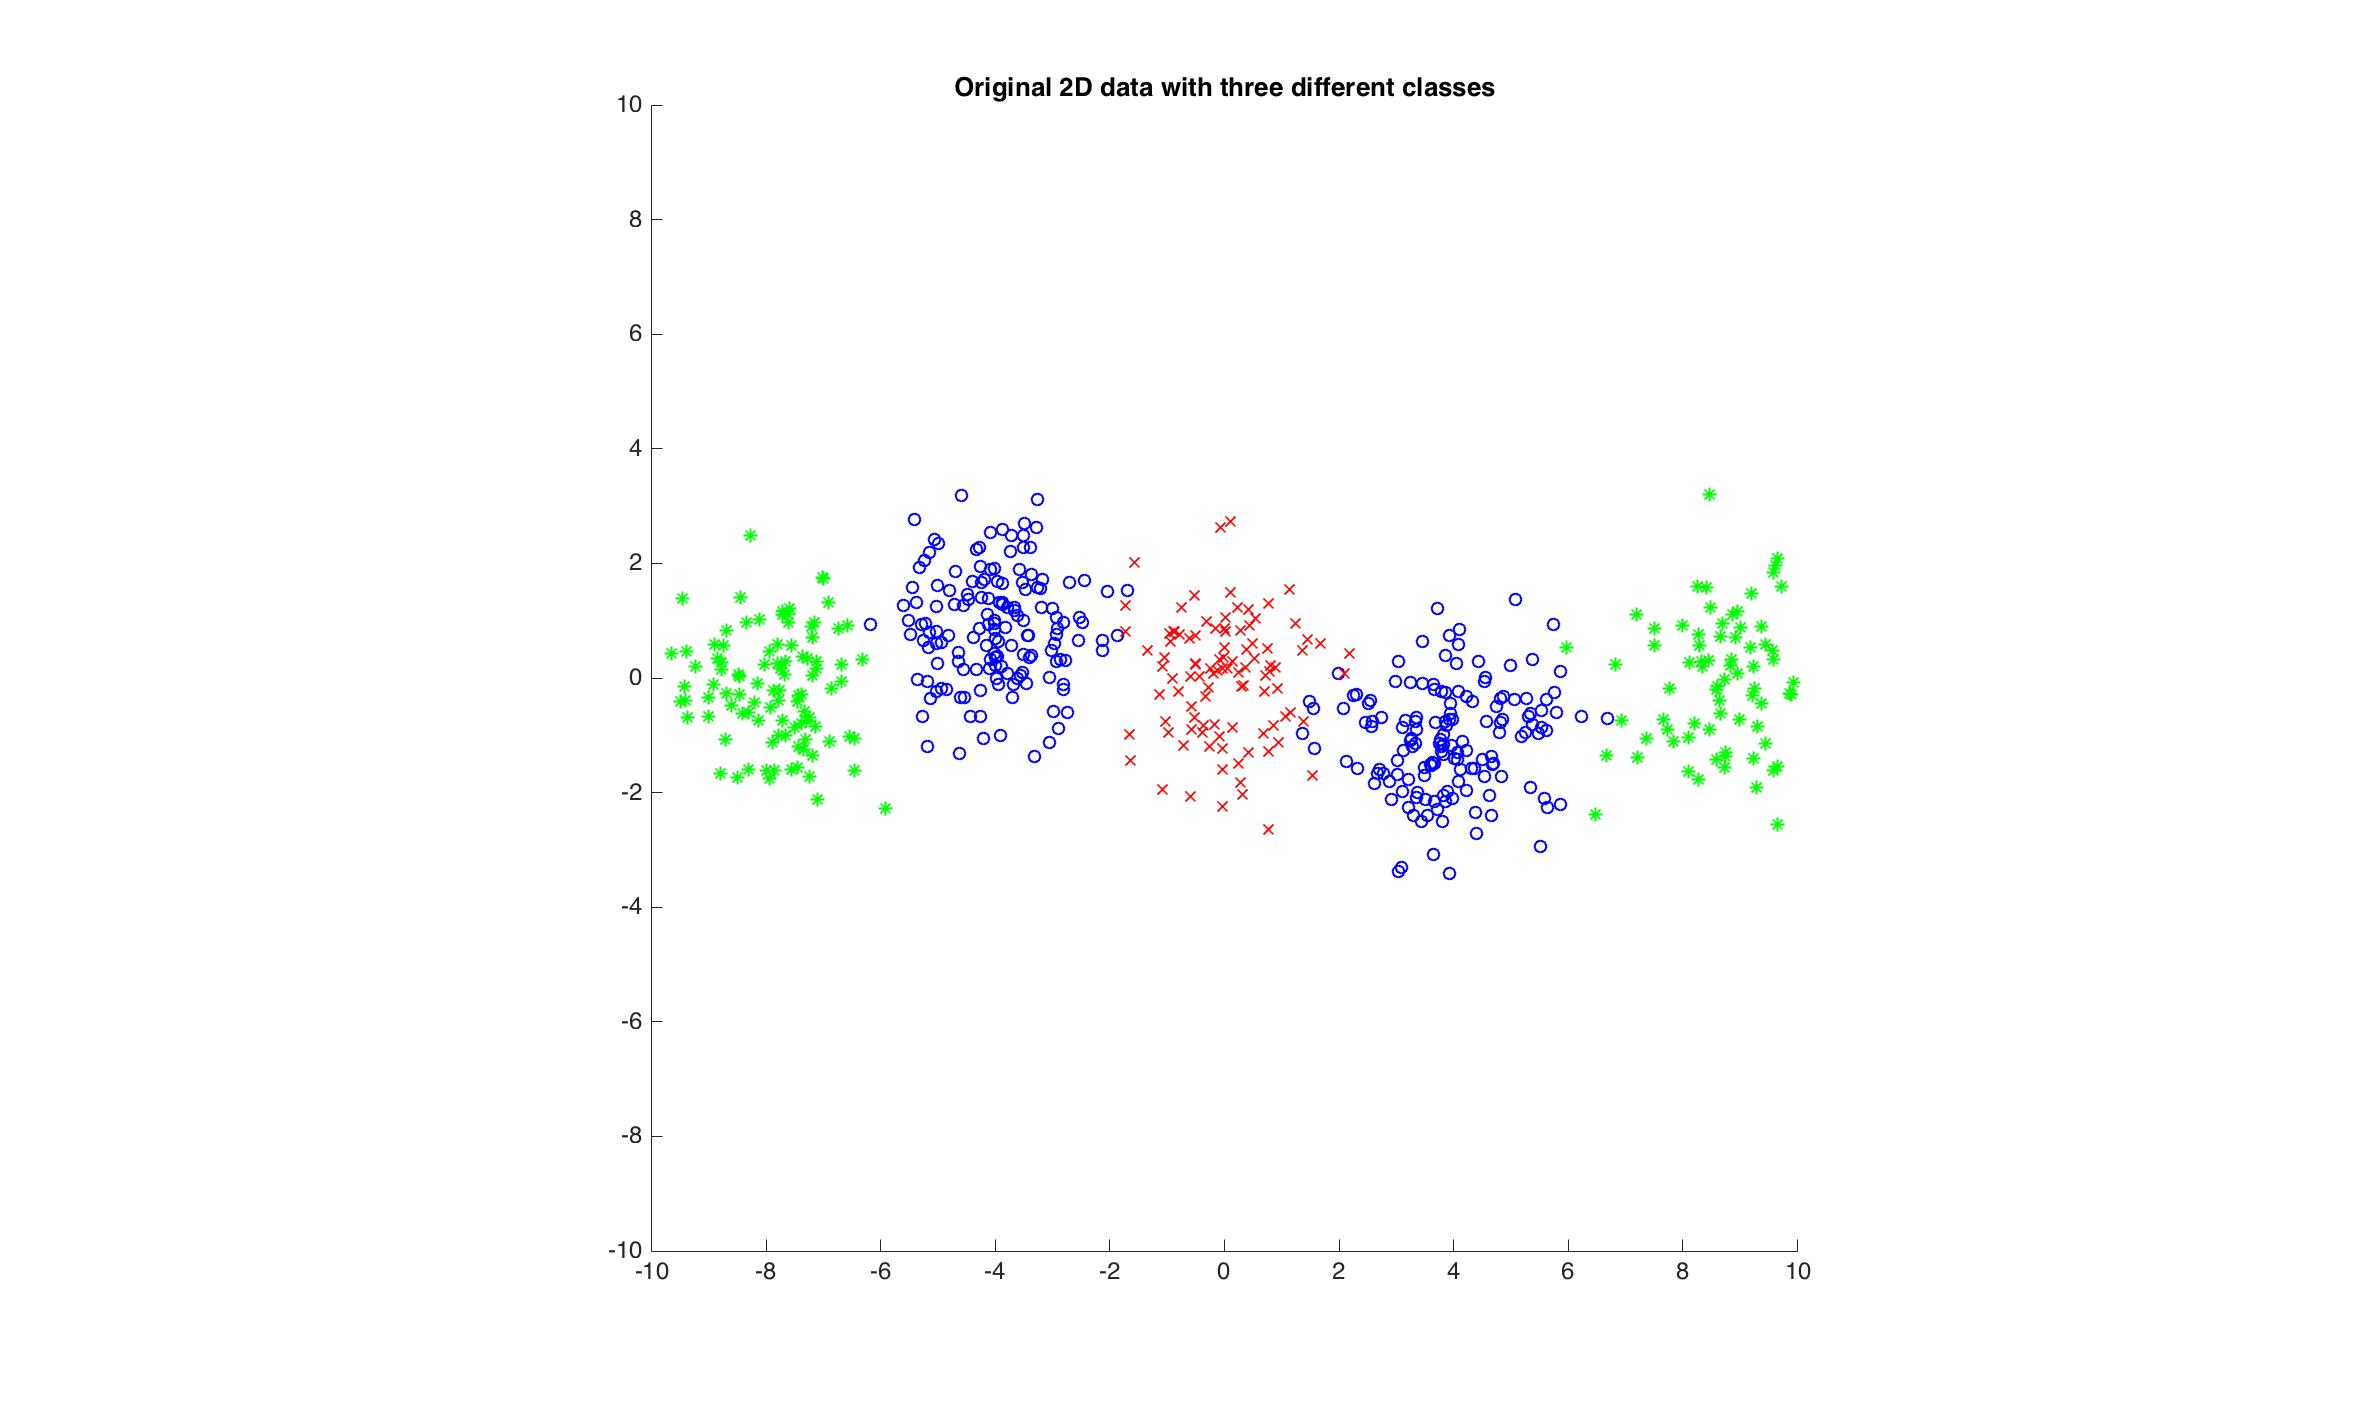
\includegraphics[width=1\linewidth]{/Users/JohnsonJohnson/Downloads/thesis_1/Figures/KLFDAdemo1.jpg}
%\caption{Example of five clusters belong to three classes}
%\vspace{0em}
%\end{figure} 
%\label{KLFDAdemo1}
%
%\begin{figure}[H]
%\centering
%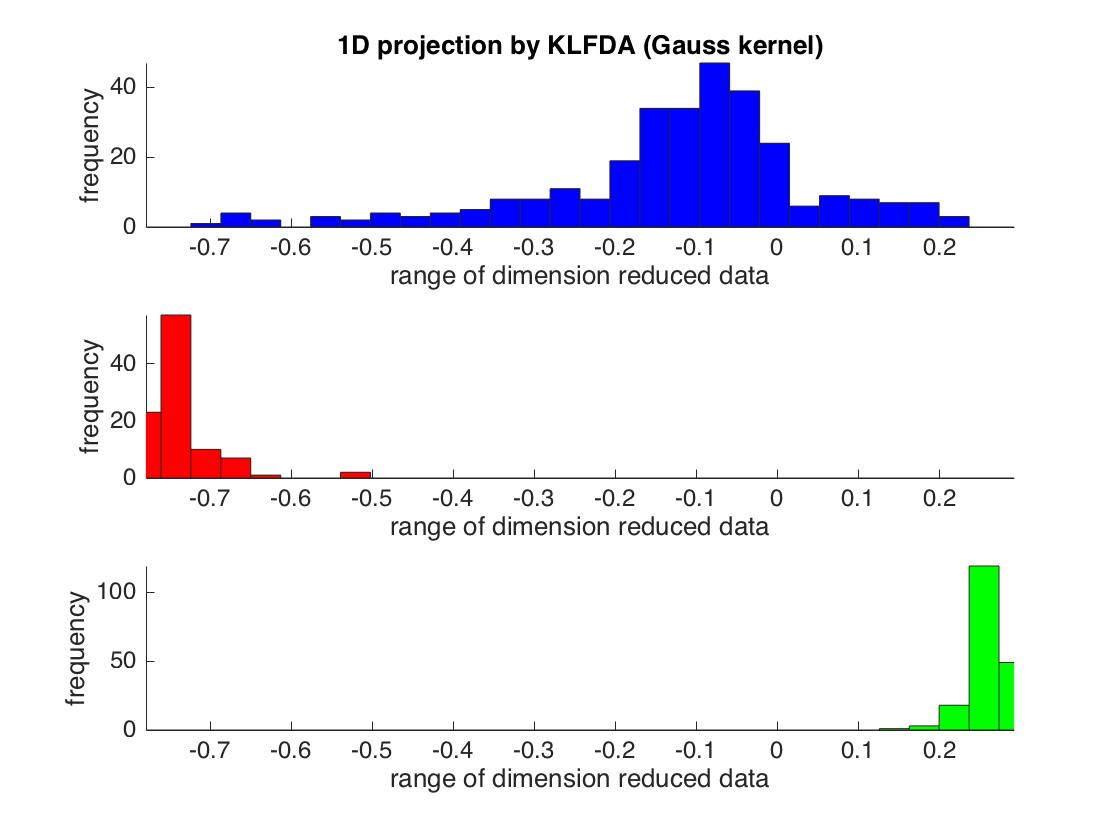
\includegraphics[width=1\linewidth]{/Users/JohnsonJohnson/Downloads/thesis_1/Figures/KLFDAdemo2.jpg}
%\caption{1-D distribution of dimension reduced data  with gaussian kernel}
%\vspace{-1em}
%\end{figure} 
%\label{KLFDAdemo2}
%
%\begin{figure}[H]
%\centering
%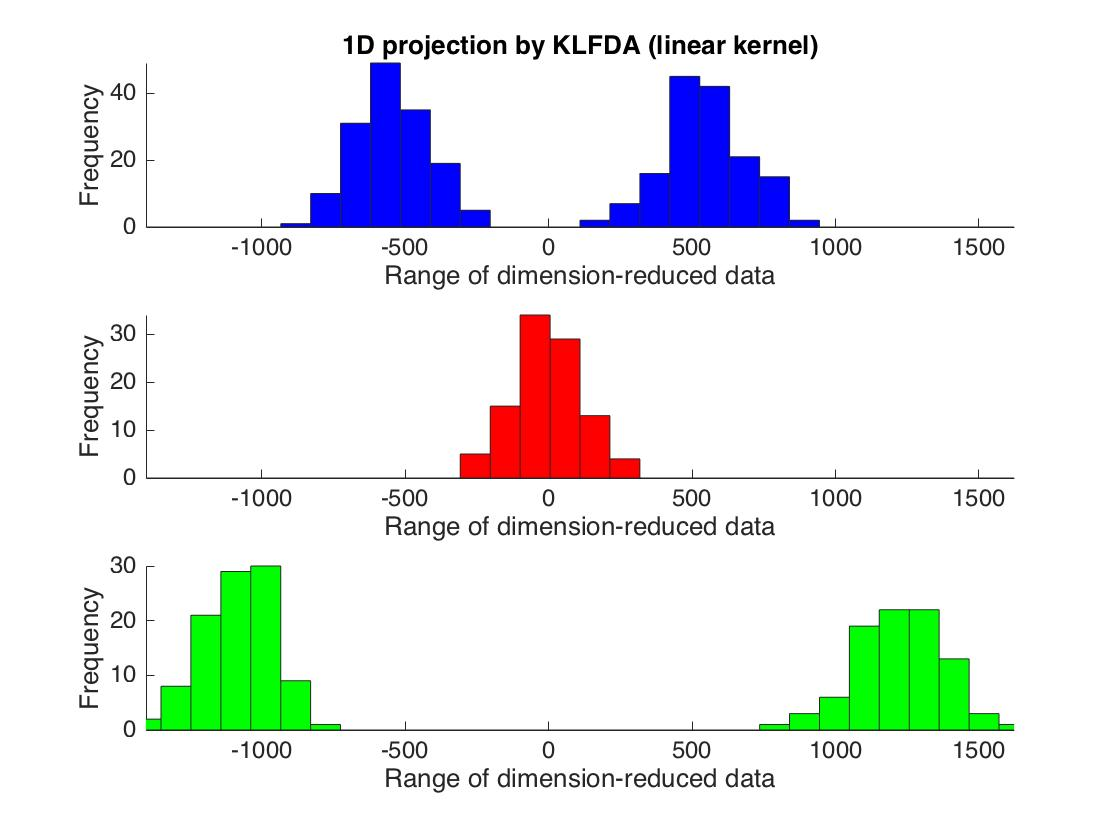
\includegraphics[width=1\linewidth]{/Users/JohnsonJohnson/Downloads/thesis_1/Figures/KLFDAdemo3.jpg}
%\caption{1-D distribution of dimension reduced data  with linear kernel}
%\vspace{-1em}
%\end{figure} 
%\label{KLFDAdemo3}
%%\begin{figure}[H]
%%\centering
%%\begin{minipage}[t]{0.5\linewidth}
%%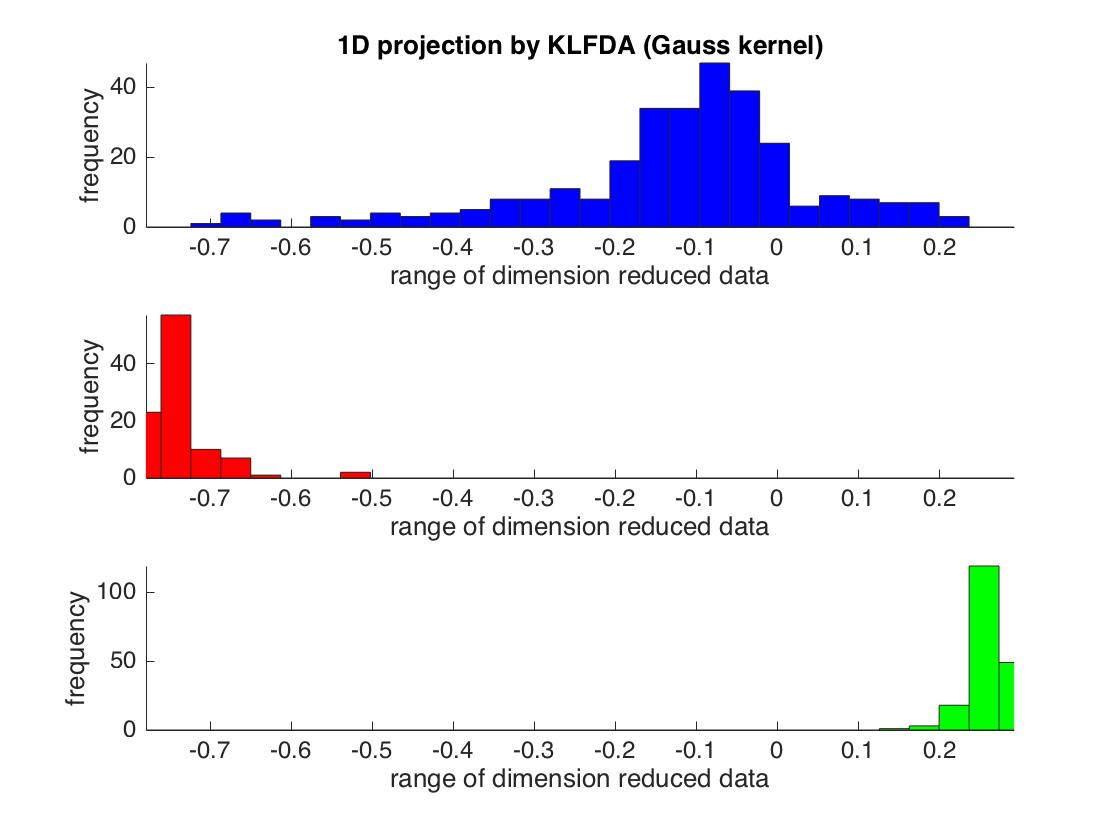
\includegraphics[width=2.7in]{/Users/JohnsonJohnson/Downloads/thesis_1/Figures/KLFDAdemo2.jpg}
%%%\caption{RGB patch}
%%\label{fig:side:a}
%%\end{minipage}%
%%\begin{minipage}[t]{0.5\linewidth}
%%\centering
%%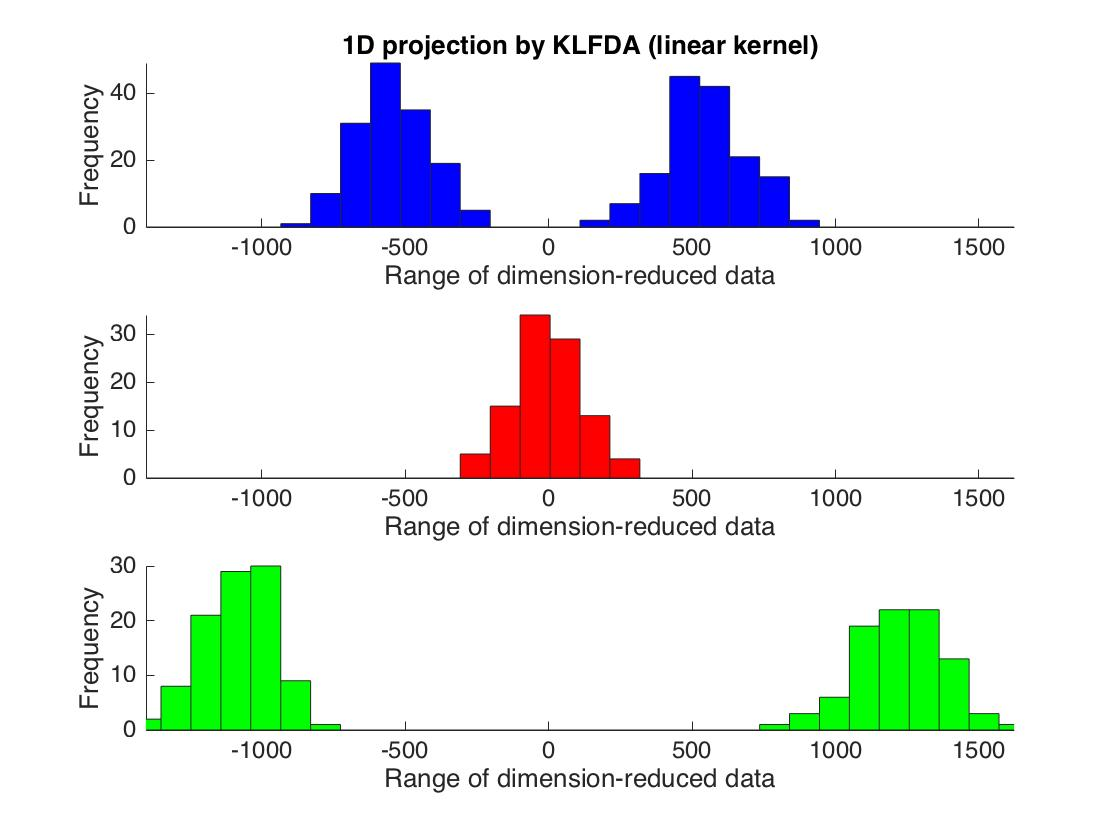
\includegraphics[width=2.7in]{/Users/JohnsonJohnson/Downloads/thesis_1/Figures/KLFDAdemo3.jpg}
%%%\caption{GBR patch}
%%\label{fig:side:b}
%%\end{minipage}
%%\caption{A comparison of two patches with same entropy but different color distribution}
%%\end{figure}
%
%
%
%
%
%

\chapter{Metric learning on subspace}



\section{Mahalanobis distance}
The Mahalanobis distance based metric learning has received much attention in similarity computing. The Mahanalobis distance of two observations $\bm{x} $ and $\bm{y}$ is defined as
\begin{equation}
D(\bm{x},\bm{y}) = (\bm{x} - \bm{y})^T\bm{M}(\bm{x} - \bm{y}), 
\end{equation}
where $\bm{x}$ and $\bm{y} $ are $d\times1$ observation vectors, $\bm{M}$ is a positive-semidefinite matrix. Since $\bm{M}$ is positive-semidefinite, $\bm{M}$ can be decomposed as $\bm{M} = \bm{W}^T\bm{W}$, and Mahanalobis distance can also be written as 
\begin{equation}
D(\bm{x},\bm{y}) = (\bm{x} - \bm{y})^T\bm{W}^T\bm{W}(\bm{x} - \bm{y})= ||\bm{W}(\bm{x} - \bm{y})||
\end{equation}
 Therefore, Mahanalobis distance can be regarded as a variant of Euclidean distance. There are many methods proposed for metric learning[ ]. 
 
 \section{Gradient descent optimization}
 Given a multivariate function $F(\bm{x})$, if $f(\bm(x))$ is continuous and differentiable in the neighbour of point $\bm{x}$ for all $\bm{x}$, then $f(\bm(x))$ decreases fastest in the direction of negative gradient of $F$ at $\bm{x}$. To compute the minimum of $F(\bm{x})$, an iterative method can be use by updating $F$ with respect to $\bm{x}$. If the updating step $\lambda$ is small enough, by updating $\bm{x}$ with 
 \begin{equation}
 \bm{x}_{t+1} = \bm{x}_{t} - \lambda \bm{G}
 \end{equation}
 
 we have 
  \begin{equation}
 F(\bm{x}_{t+1}) \ge F(\bm{x}_t).
  \end{equation}
 
 \section{Metric learning based on sample pairs distance comparison}
 Inspired by [], in this paper, a similar metric learning based on iteration computation is used. For a  sample descriptor $\bm{x}_i$,  its positive pairwise set is defined as $\{\bm{x}_i,\bm{x}_j\}$, where class ID $y_i = y_j$. Also the negative pairwise set can be defined as $\{\bm{x}_i,\bm{x}_j\}$, where $y_i \ne y_j$. Similar with [PRDC], this method is also based on similarity comparison. The difference is in [PRDC], for all possible positive and negative pairs, the distance between positive pairs must be smaller than the distance between negative pairs. Since it has to compare possible positive and negative pairs, computation complexity will be quite huge.  To decrease complexity, a simplified version is proposed as the top-push distance metric learning[ ].  Since re-identification is a problem of ranking, it is desired that the rank-1 descriptor should be the right match. Given a Mahanalobis matrix $\bm{M}$, for samples $\bm{x}_i, i = 1,2,3,\cdots,n$, $n$ is the number of all samples, the requirement is distance between positive pair should be smaller than the minimum of all negative distance. This can be denoted as 
 \begin{equation}
 D(\bm{x}_i,\bm{x}_j) + \rho < \min D(\bm{x}_i,\bm{x}_k), y_i = y_j, y_i\ne y_k.
 \end{equation}
 $\rho$ is a slack variable and $\rho \in [0,1]$. This equation can be transformed into a optimization problem with respect to descriptor $\bm{x}_i$ as
 \begin{equation}
 \min \sum_{y_i = y_j} \max \{D(\bm{x}_i,\bm{x}_j) -  \min_{ y_i\ne y_k} D(\bm{x}_i,\bm{x}_k)  + \rho \}.
 \end{equation}
 
 However, the equation above only penalize the interclass distance. Another term is needed to penalize intra class distance. That is, to make the sum of intraclass distance as small as possible. This term is denoted as 
 \begin{equation}
 \min \sum D(\bm{x}_i,\bm{x}_j),y_i = y_j.
 \end{equation}
 
 To combine equations above, a ratio factor $\alpha$ is assigned to equation [] so that the target function can be denote as 
  \begin{equation}
  \begin{aligned}
 f(\bm{M}) = (1-\alpha)\sum_{\bm{x}_i,x_j,\bm{y}_i=y_j} D(\bm{x}_i,\bm{x}_j) + \\
  \alpha \sum_{\bm{x}_i,\bm{x}_j,y_i=y_j}\max\{{D(\bm{x}_i,\bm{x}_j)-\min_{y_i\ne y_k}{D(\bm{x}_i,\bm{x}_k)}+\rho,0}\}
 \end{aligned}
 \end{equation}
 In this way the problem is transformed to an optimization problem. Notice that equation 16 can be denoted as 
 \begin{equation}
 D(\bm{x},\bm{y}) = (\bm{x} - \bm{y})^T\bm{M}(\bm{x} - \bm{y}) = trace(\bm{M}\bm{X}_{i,j})
 \end{equation}
 where $\bm{X}_{i,j} = \bm{x}_i*\bm{x}_j^T$, and $trace$ is to compute matrix trace. Therefore, equation 21 can be transformed as follow,
 \begin{equation}
 \begin{aligned}
 f(\bm{M}) = (1-\alpha)\sum_{y_i = y_j}trace(\bm{M}\bm{X}_{i,j}) \\
  + \alpha \sum_{y_i = y_j,y_i\ne y_k}\max\{trace(\bm{M}\bm{X}_{i,j}) - trace(\bm{M}\bm{X}_{i,k} )+ \rho,0\}
 \end{aligned}
 \end{equation}
 
 To minimize equation 23, the gradient descent method is used. The gradient respect to $\bm{M}$ is computed as
 \begin{equation}
 \begin{aligned}
\bm{G} =  \frac{\partial f}{\partial \bm{M}} = (1-\alpha) \sum_{y_i = y_j} \bm{X}_{i,j} \\
 + \alpha \sum_{y_i = y_j, y_i \ne y_k}(\bm{X}_{i,j} - \bm{X}_{i,k})
 \end{aligned}
 \end{equation}
 
 The iteration process can be summarized as following \\
 \begin{table}
 \centering
 \begin{tabular}{l}
 \hline 
 \multicolumn{1}{l}{\textbf{Gradient optimization algorithm for target function}} \\
 \hline
 \textbf{Input} Descriptors of training person pairs \\
 \textbf{Output} A SPD matrix\\
 \textbf{Initialization} \\
 Initialize $\bm{M}$ with eye matrix $\bm{I}$; \\
 Compute the initial target function value $f_0$ with $\bm{M}_0$;\\
 Iteration count  $t = 0$;\\

 \textbf{while}(not converge)\\
 \indent Update $t =  t + 1$;\\
 \indent Update gradient $\bm{G}_{t+1}$ with equation 24;\\
 \indent Update $\bm{M}$ with equation : $\bm{M}_{t+1} = \bm{M}_{t} - \lambda\bm{G}_t$\\
 \indent Project $\bm{M}_{t+1}$ to the positive semi-definite space \\ 
 \indent \indent by $\bm{M}_{t+1}= \bm{V}_{t+1}\bm{S}_{t+1}\bm{V}^T_{t+1}$;\\
 \indent Update the target value $f|_{\bm{M} = \bm{M}_{t+1}}$;\\
 \textbf{end while}  \\
 return $\bm{M}$\\
 \hline

 \end{tabular} 
 \end{table}


 
 
 
 
 
 
\chapter{Experiment Settings}


\section{Datasets and evaluation settings}

\noindent \textbf{VIPeR} dataset is the most used dataset in person re-identification. In this dataset there are 632 different individuals and for each person there are two outdoor images from different viewpoints. All the images are scaled into $48\times128$. In this experiment the we randomly select 316 individuals from cam A and cam B as the training set, the rest images in cam A are used as probe images and those in cam B as gallery images. This process is repeated 10 times to reduce error.\\
%\textbf{ETHZ dataset} Three video sequences are contained in this dataset. In ETHZ there are respectively 83,35,28 persons in each sequences. All those images are outdoor and the camera is moving with the pedestrian. Images are in different sizes and may needed to resized. All those images of a certain person is shot with the same moving camera. In this paper, for each person two random images are selected as the training pair and another two random images are selected as the gallery and probe image.\\
\textbf{CUHK1} dataset contains 971 identities from two disjoint camera views. The cameras are static in each pair of view and images are listed in the same order. For each individual, there are two images in each view. All images are scaled into $60\times160$. In this paper, we randomly select 485 image pairs as training data and the rest person pairs are used for test data. 
\begin{figure}[H]
\begin{raggedleft}
\includegraphics[width=1\linewidth]{/Users/JohnsonJohnson/Downloads/thesis_1/Figures/CUHKimagesdemo.jpg}
\vspace{-3em}
\caption{Pedestrians in prid\_450 dataset}
\end{raggedleft}
\end{figure}
\textbf{Prid\_2011} dataset consists of images extracted from multiple person trajectories recorded from two different, static surveillance cameras. Images from these cameras contain a viewpoint change and a stark difference in illumination, background and camera characteristics. Camera view A shows 385 persons, camera view B shows 749 persons. The first 200 persons appear in both camera views, The remaining persons in each camera view complete the gallery set of the corresponding view. Hence, a typical evaluation consists of searching the 200 first persons of one camera view in all persons of the other view. This means that there are two possible evaluation procedures, either the probe set is drawn from view A and the gallery set is drawn from view B. In this paper, we randomly select 100 persons that appeared in both camera views as training pairs, and the remaining 100 persons of the 200 person pairs from camera A is used as probe set while the 649 remaining persons from camera B are used for gallery images.\\
%\begin{figure}[H]
%\begin{raggedleft}
%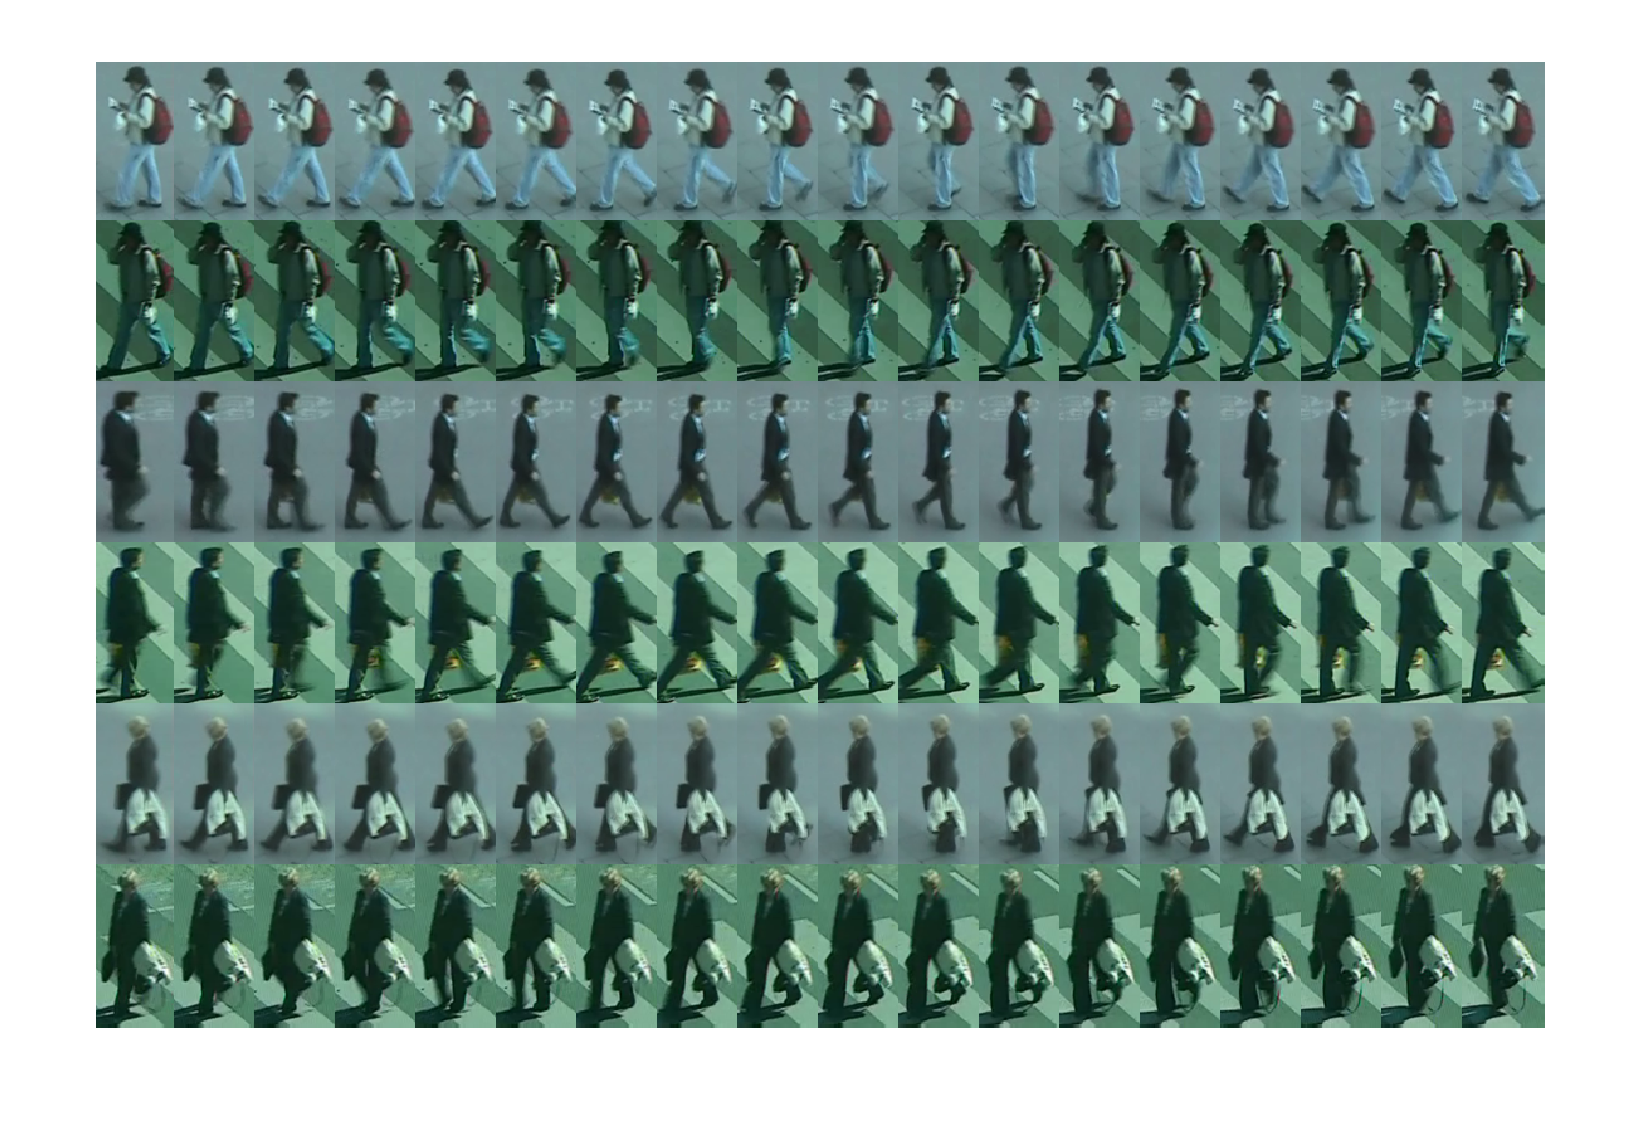
\includegraphics[width=1\linewidth]{/Users/JohnsonJohnson/Downloads/thesis_1/Figures/Multishots.eps}
%\vspace{-3em}
%\caption{Pedestrians in prid\_2011 dataset}
%\end{raggedleft}
%\end{figure}
%\label{Prid\_2011 pedestrians}
\textbf{Prid\_450s} dataset contains 450 image pairs recorded from two different, static surveillance cameras. Additionally, the dataset also provides an automatically generated, motion based foreground/background segmentation as well as a manual segmentation of parts of a person. The images are stored in two folders that represent the two camera views. Besides the original images , the folders also contain binary masks obtained from motion segmentation, and manually segmented masks. In this test, we randomly select 225 persons from each of two camera views as the training set, and the remaining persons are left as gallery and probe images. 
\begin{figure}[H]
\begin{raggedleft}
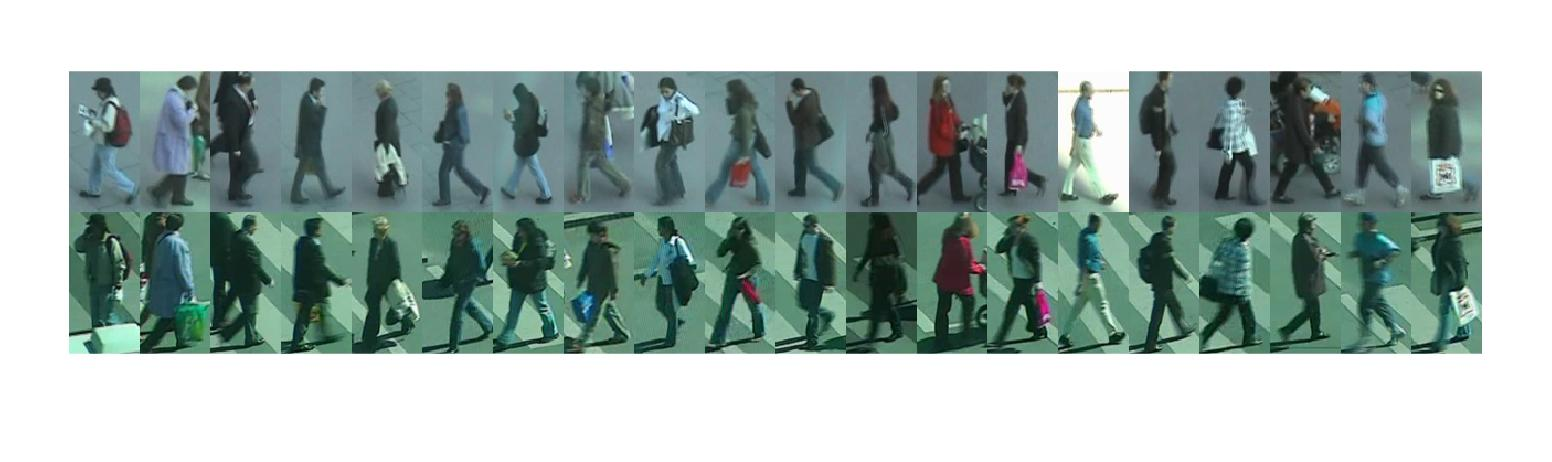
\includegraphics[width=1\linewidth]{/Users/JohnsonJohnson/Downloads/thesis_1/Figures/Prid450sImages.jpg}
\vspace{-3em}
\caption{Pedestrians in prid\_450s dataset}
\end{raggedleft}
\end{figure}

\textbf{GRID} There are two camera views in this dataset. Folder probe contains 250 probe images captured in one view (file names starts from 0001  to 0250). Folder gallery contains 250 true match images of the probes (file names starts from 0001  to 0250). Besides, in gallery folder there are a total of 775 additional images that do not belong to any of the probes (file name starts with 0000). These extra images should be treated as a fixed portion in the testing set during cross validation. In this paper, we randomly select 125 persons from those 250 persons appeared in both camera views as training pairs, and the remaining persons in probe folder is used as probe images while  the remaining 125 persons and those 775 additional persons from gallery folder are used as gallery images. A brief summarization of test settings is in Table \ref{Settings}.

\begin{figure}[H]
\begin{raggedleft}
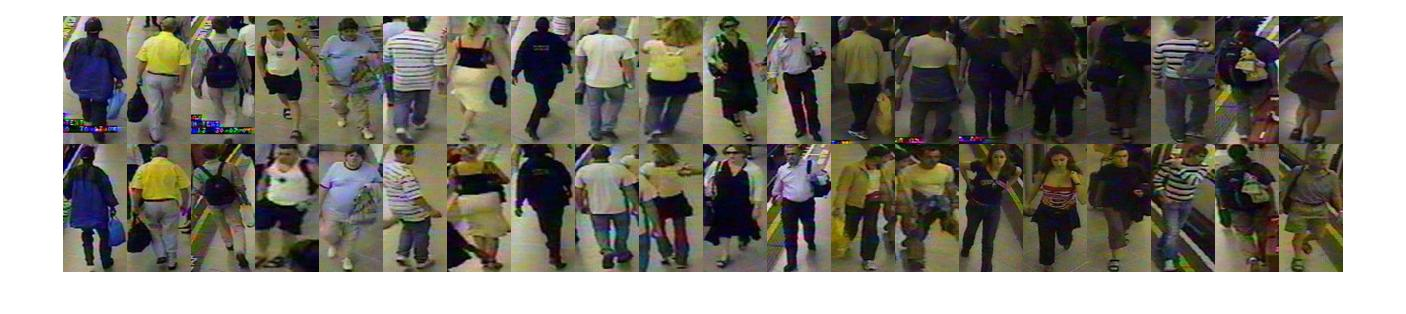
\includegraphics[width=1\linewidth]{/Users/JohnsonJohnson/Downloads/thesis_1/Figures/GRIDimagesdemo.jpg}
\vspace{-3em}
\caption{Pedestrians in GRID dataset}
\end{raggedleft}
\end{figure}
%-------------------------------------------------
\begin{table}[H]
\centering
\caption{Testing setting for different datasets}
\label{Settings}
%\centering
\begin{tabular}{|l|c|c|c|c|c|}
\hline
Dataset&training&probe&gallery&cam\_a&cam\_b\\
\hline
VIPeR&316&316&316&632&632\\
\hline
CUHK1&485&486&486&971&971\\
\hline
Prid\_2011&100&100&649&385&749\\
\hline
Prid\_450s&225&225&225&450&450\\
\hline
GRID&125&125&900&250&1025\\
\hline
\end{tabular}\\ 
\end{table}
%-----------------------------------------------------------------------------------------------------------------------------------------------------------------------------------------------------------------------------------------------------
\section{The influence of mean removal and $L_2$ normalization}
In \cite{GOG}, mean removal and $L_2$  normalization is found to improve performance by $5.1\%$. The reason for this is mean removal and normalization can reduce the impact of extremas of descriptors. When testing proposed metric learning, we find the mean removal can slightly improve performance. A comparison between performance of original descriptors and preprocessed descriptors is shown in Tables \ref{table:compMN1}, \ref{table:compMN2}, \ref{compMN3}, \ref{compMN4}, \ref{compMN5}, all those datasets are tested by proposed metric. The original GOG means no mean removal and normalization. It shows that the mean removal and normalization has a slight improvement around 0.5\% on the performance on all five datasets. Since preprocessing are required to test XQDA, the mean removal and normalization are applied on descriptors in this experiment. 

\begin{table}[H]
\centering
\caption{The influence of data preprocessing on VIPeR}
\label{table:compMN1}
\begin{tabular}{|l|c|c|c|c|c|}
\hline
 & \multicolumn{5}{|c|}{Rank(\%)} \\
 \hline
Terms  &1 &5 & 10 &15& 20\\
\hline
Original GOG &43.01&74.91& 84.87& 89.81& 93.32 \\
\hline
Preprocessed GOG$_\text{rgb}$ &43.77&74.84&85.25& 90.32&93.89\\
 \hline
Original GOG$_\text{fusion}$ &48.77&77.47&87.41&91.52&94.27\\
\hline
Preprocessed GOG$_\text{fusion}$ &48.32&76.90&87.78&91.93& 94.49\\
 \hline

\end{tabular}
\end{table}


%---------------------------------------------
\begin{table}[H]
\centering
\caption{The influence of data preprocessing on CUHK1}
\label{table:compMN2}
\begin{tabular}{|l|c|c|c|c|c|}
\hline
 & \multicolumn{5}{|c|}{Rank(\%)} \\
 \hline
Terms  &1 &5 & 10 &15& 20\\
\hline
Original GOG$_\text{rgb}$&56.11&83.77&90.10& 92.65&94.28 \\
\hline
Preprocessed GOG$_\text{rgb}$ &55.91&84.24&90.41& 93.15&94.67\\
 \hline
Original GOG$_\text{fusion}$ &57.10&84.65& 90.35& 92.88&94.65\\
\hline
Preprocessed GOG$_\text{fusion}$ &56.67&84.49& 90.51& 93.31&94.84\\
 \hline
 
\end{tabular}
\end{table}

%---------------------------------------------
\begin{table}[H]
\centering
\caption{The influence of data preprocessing on prid\_2011}
\label{compMN3}
\begin{tabular}{|l|c|c|c|c|c|}
\hline
 & \multicolumn{5}{|c|}{Rank(\%)} \\
 \hline
Terms  &1 &5 & 10 &15& 20\\
\hline
Original GOG$_\text{rgb}$&24.80& 52.10& 63.20& 69.90& 72.90\\
\hline
Preprocessed GOG$_\text{rgb}$ &23.80& 52.20& 63.50& 70.20& 73.50\\
\hline
Original GOG$_\text{fusion}$ &32.20& 56.60& 67.00& 73.10& 77.70\\
\hline
Preprocessed GOG$_\text{fusion}$ &32.30& 57.40& 66.30& 73.40& 78.00\\
 \hline
 
\end{tabular}
\end{table}

%---------------------------------------------
\begin{table}[H]
\centering
\caption{The influence of data preprocessing on prid\_450s}
\label{compMN4}
\begin{tabular}{|l|c|c|c|c|c|}
\hline
 & \multicolumn{5}{|c|}{Rank(\%)} \\
 \hline
Terms  &1 &5 & 10 &15& 20\\
\hline
Original GOG$_\text{rgb}$&60.93& 84.31& 91.29& 94.00& 96.18\\
\hline
Preprocessed GOG$_\text{rgb}$ &60.71& 84.53& 91.29& 94.13& 96.27\\
\hline
Original GOG$_\text{fusion}$ &63.07& 86.67& 92.53& 95.20& 96.98\\
\hline
Preprocessed GOG$_\text{fusion}$ &62.80& 86.58& 92.36& 95.29& 96.89\\
 \hline
 
\end{tabular}
\end{table}

%---------------------------------------------
\begin{table}[H]
\centering
\caption{The influence of data preprocessing on GRID}
\label{compMN5}
\begin{tabular}{|l|c|c|c|c|c|}
\hline
 & \multicolumn{5}{|c|}{Rank(\%)} \\
 \hline
Terms  &1 &5 & 10 &15& 20\\
\hline
Original GOG$_\text{rgb}$&22.96& 41.92& 51.68& 58.72& 64.64\\
\hline
Preprocessed GOG$_\text{rgb}$ &22.64& 43.68& 52.00& 59.04& 65.04\\
\hline
Original GOG$_\text{fusion}$ &24.32& 44.56& 54.80& 62.40& 66.64\\
\hline
Preprocessed GOG$_\text{fusion}$ &23.92& 44.64& 54.88& 62.32& 66.40\\
 \hline
 
\end{tabular}
\end{table}


%--------------------------------------------------
\section{Parameters setting}
In this experiment, there are a few parameters for the iteration computing including slack variable $\rho$, maximal iteration $T$, gradient step $\lambda$, the interclass and intraclass limitation factor $\alpha$ and the updating ratio $\beta$. Firstly the slack variable $\rho$ is initialized as 1 to ensure the minimum interclass distance is 1 larger than intraclass distance at least. The step size of gradient updating $\lambda$ is initialized as 0.01. When target value $f$ increases,  $\lambda$ is scaled by a factor 0.5, and  $\lambda$ is scaled by 1.01 when target value $f$ decreases. To judge if target value converges, the threshold $\beta$ is defined as the ratio target value change versus previous target value, that is, $\beta = \frac{(f_{t+1}-f_t)}{f_t}$. According many experiment trials, when it satisfies $\beta = 10^{-5}$, the target value converges and the iteration is stopped. The maximal iteration times $t$ is set to 100 since the target value $f$ will converge in around 15 iterations.  The last parameter for the iteration is $\alpha$, to know the best value for $\alpha$, we tried 11 different values ranges from 0 to 1 with a step of 0.1, and find that the rank 1 and rank 5 scores reach maxima at interval $[0.7,0.8]$, as shown in \ref{Rank1curve} and \ref{Rank5curve}. Then another ten trials are performed with alpha ranging from $[0.7,0.8]$ with a step of 0.01. The best $\alpha$ value should have as large top rank scores as possible and at last we find that the optimal value for $\alpha$ is 0.76. A form of all parameters are shown in Table \ref{ParametersSetting}.
%-------------------------------------------------
\begin{figure}[H]
\begin{raggedleft}
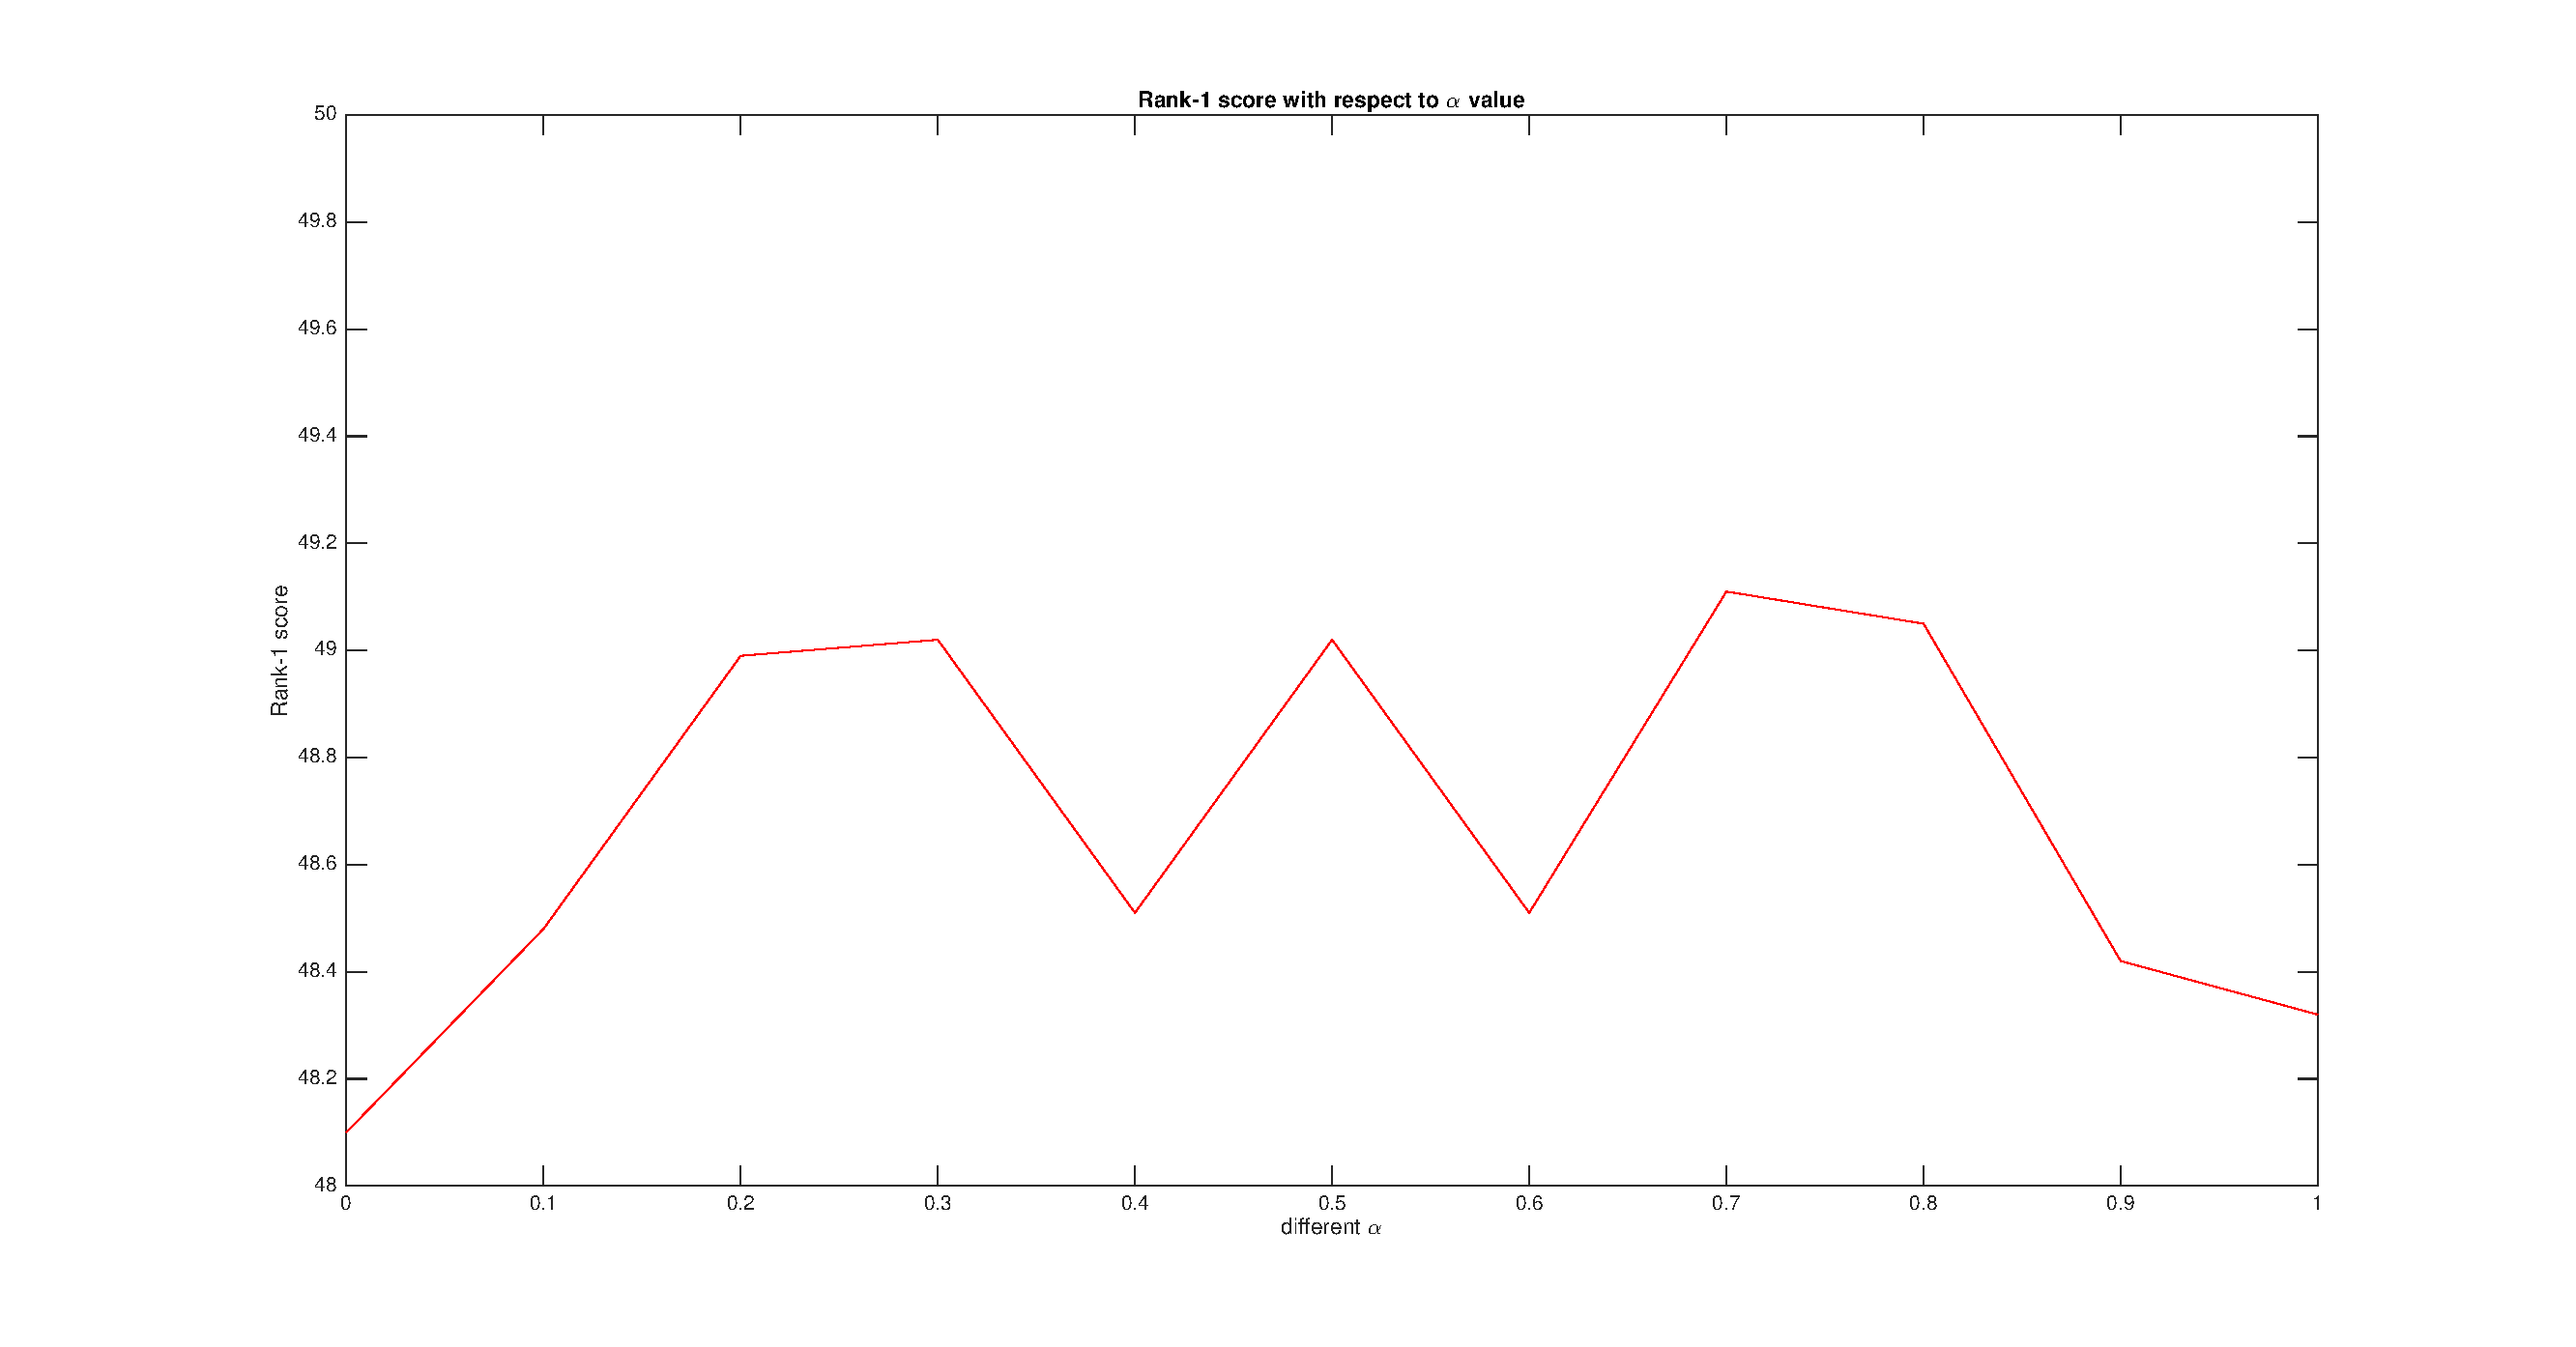
\includegraphics[width=1\linewidth]{/Users/JohnsonJohnson/Downloads/thesis_1/Figures/Rank1scoresAlpha.eps}
\vspace{-3em}
\caption{Rank 1 scores with respect to $\alpha$ on VIPeR}
\label{Rank1curve}
\end{raggedleft}
\end{figure}
%-------------------------------------------------
\begin{figure}[H]
\begin{raggedleft}
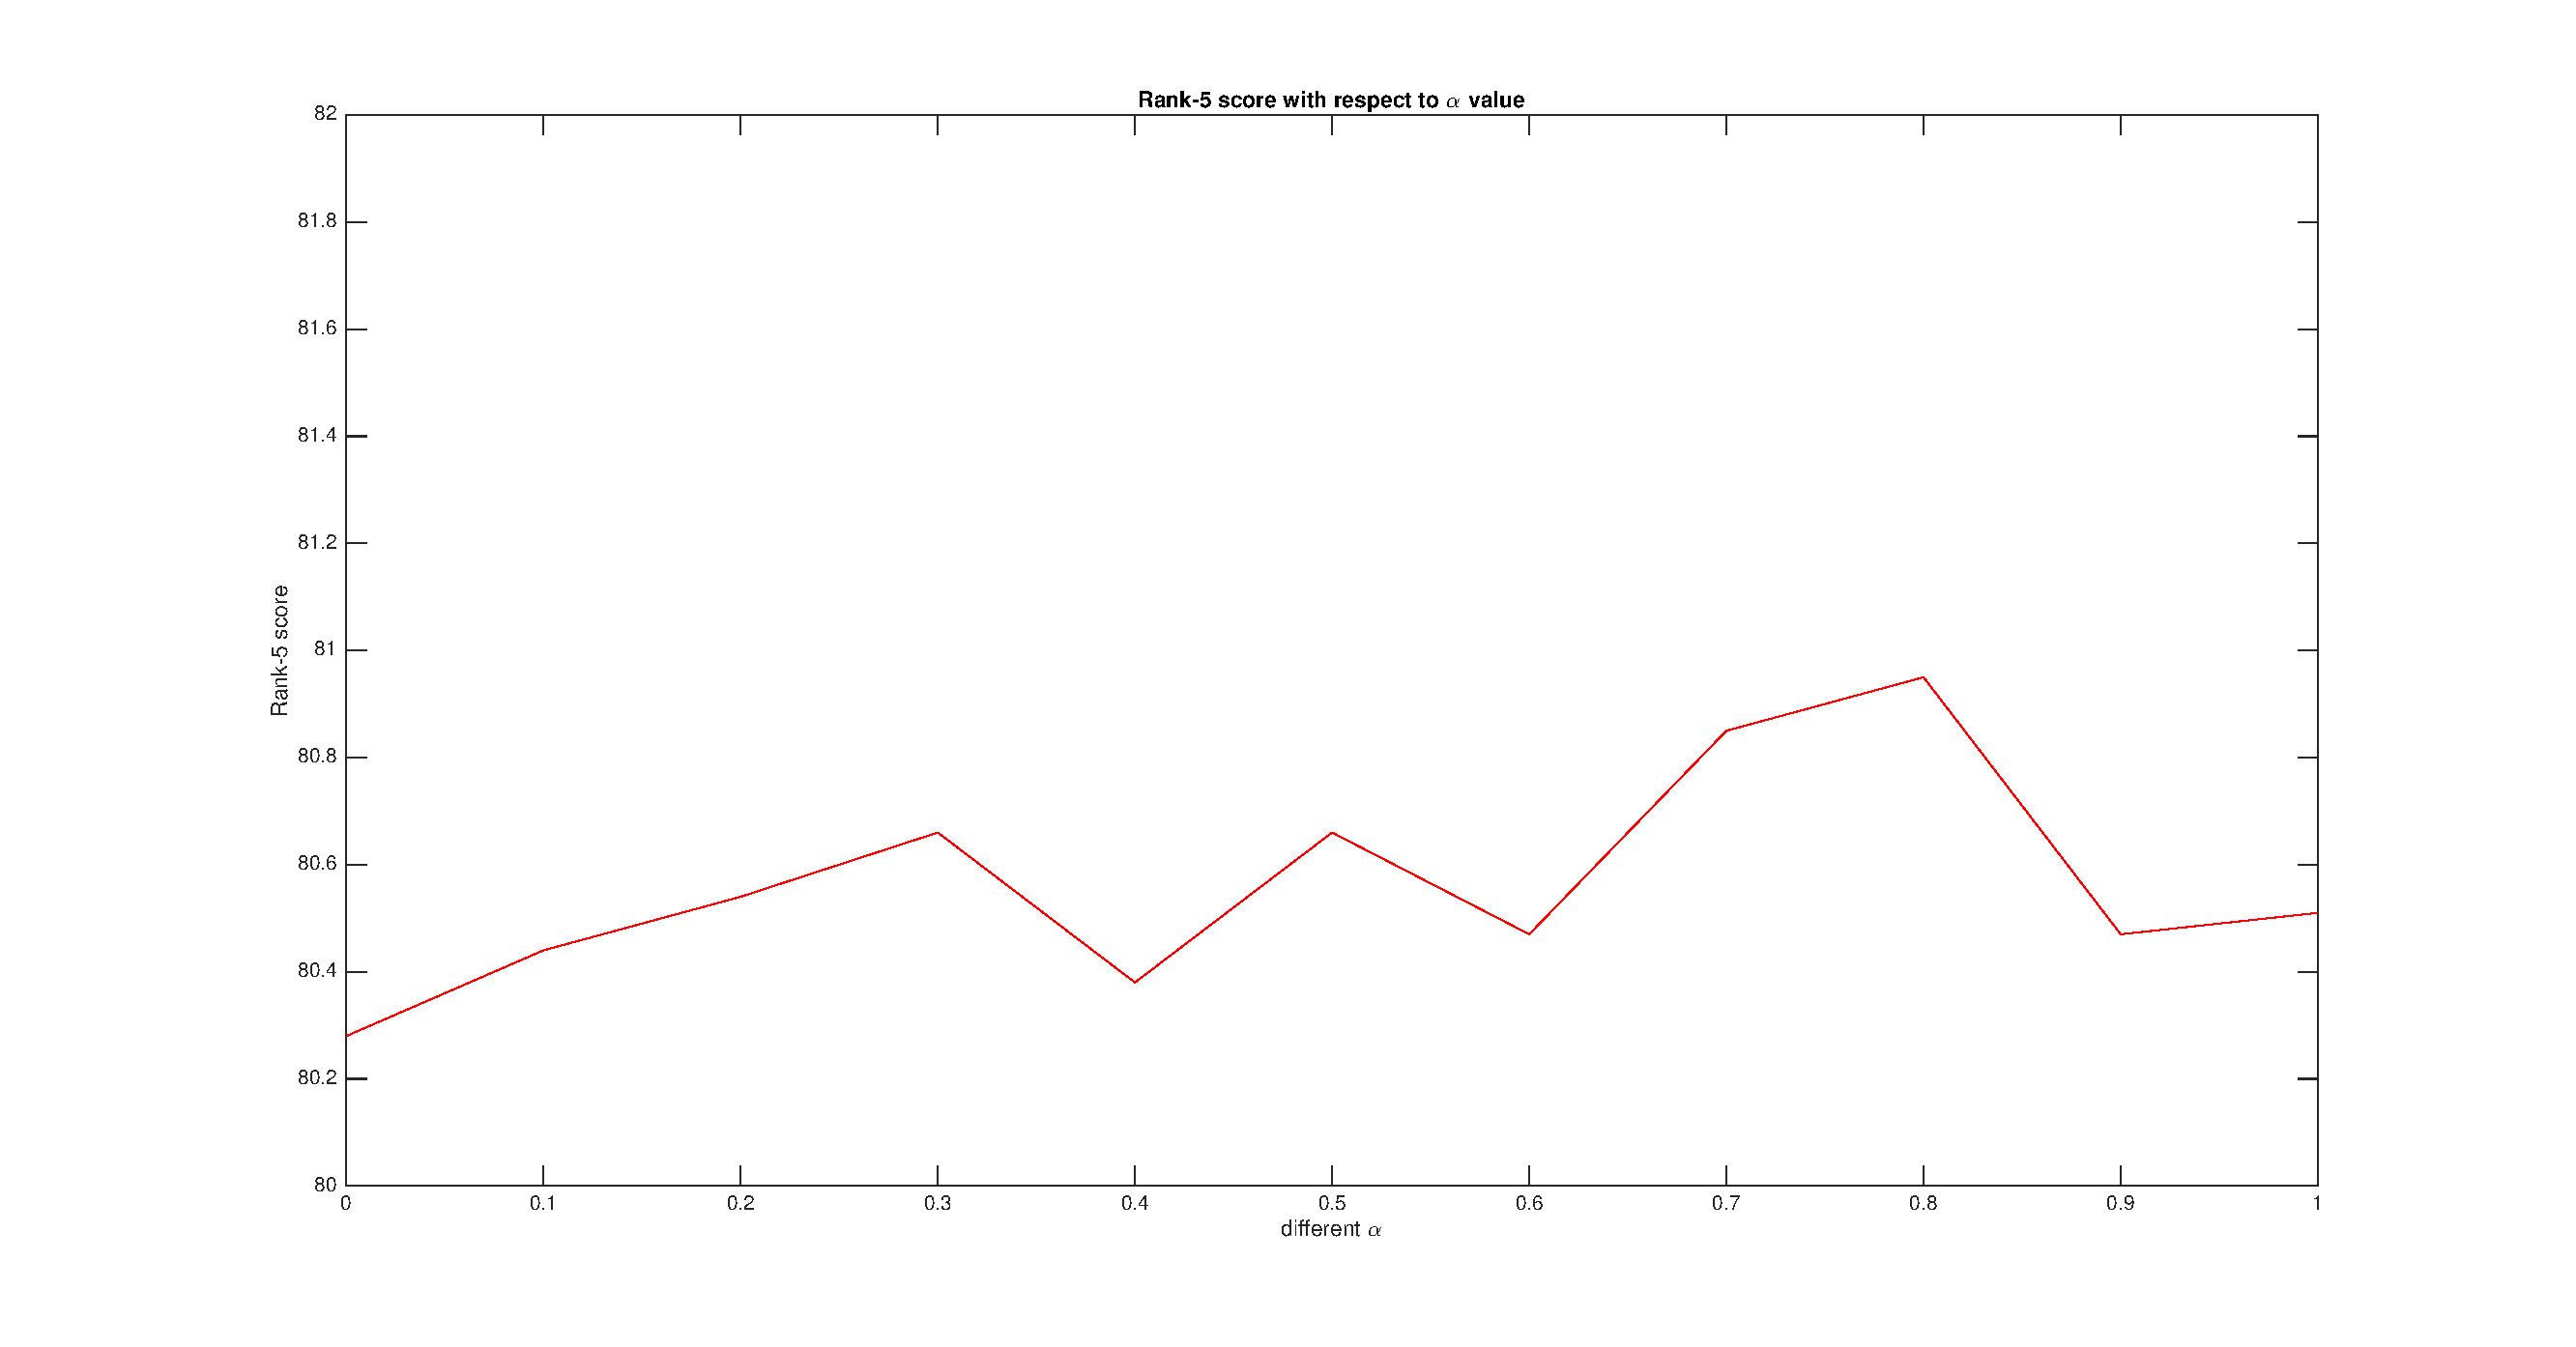
\includegraphics[width=1\linewidth]{/Users/JohnsonJohnson/Downloads/thesis_1/Figures/Rank5scoresAlpha.eps}
\vspace{-3em}
\caption{Rank 5 scores with respect to $\alpha$ on VIPeR}
\label{Rank5curve}
\end{raggedleft}
\end{figure}
%-------------------------------------------------

\begin{table}[H]
\centering
\caption{Parameters setting}
\label{ParametersSetting}
\begin{tabular}{|l|c|c|c|c|c|}
\hline
Paramters &$\alpha$&$\beta$&$\lambda$&$t$& $\rho$\\
\hline
Values &0.76&$10^{-5}$&0.01&100&1\\
\hline
\end{tabular}
\end{table}


\textbf{Performance measuring} The cumulative matching curve is used to measure the descriptor performance. The score means the probability that the right match is within the top $n$ samples. A better CMC curve is expected to have a high rank-1 value and reaches 1 as fast as possible.
%\section{XQDA and NFST}


\section{Results and experiment analysis}
In this paper, we compare proposed metric with other state-of-the-art metrics including NFST \cite{NFST}, XQDA \cite{LOMO}. NFST is a metric which learn a null space for descriptors so that the the same class descriptors will be projected to  
a single point to minimize within class scatter matrix while different classes are projected to different points. This metric is a good solution to small sample problems in person re-identification. XQDA is quite similar with many other metrics, which learns a projection matrix $W$ and then a Mahanalobis SPD matrix $\bm{M}$ is learned in the subspace. Those two metric are proved to have state-of-the-art performance with many other methods. The GOG$_\text{rgb}$ in all forms stands for the hierarchical gaussian descriptor in RGB color space while GOG$_\text{fusion}$ stands for the descriptor concatenated by four different color spaces \{RGB, Lab, HSV, nRnG\}.\\
\textbf{VIPeR} A comparison form is given in Table 3. Some of recent results are also included in this form. We can find that the rank scores are better than those of NFST and XQDA in terms of both GOG$_\text{rgb}$ and GOG$_\text{fusion}$. More specifically, the rank 1, rank 5, rank 10, rank 15 and rank 20 scores of proposed metric learning are 0.76\%, 0.92\%, 1.39\%, 1.08\%, 1.52\% higher than those of GOG$_\text{rgb}$ + XQDA, and the rank 1, rank 5, rank 10, rank 15 and rank 20 GOG$_\text{fusion}$ scores of proposed metric learning are 0.35\%, -0.54\%, 0.98\%, 0.66\%, 0.79\% higher than GOG$_\text{fusion}$ + XQDA respectively. Also we can see that the proposed metric learning has a better performance than NFST. \newline 
%-----------------------------------------------------------------------VIPeR
\begin{table}[H]
\caption{Performance of different metrics on VIPeR}
\centering
 \begin{tabular}{|l|c|c|c|c|c|c|}
\hline
& \multicolumn{5}{|c|}{Rank(\%)} \\
\hline
Methods& 1 & 5 &10& 15&20\\
\hline
GOG$_\text{rgb}$+NFST& 43.23&73.16 &83.64 & 89.59&92.88\\  
\hline
GOG$_\text{rgb}$+XQDA& 43.01&73.92&83.86& 89.24& 92.37\\
\hline
%GOG$_\text{rgb}$+KLFDA&43.45 &74.68 &85.13 &90.54&93.70\\ 
%\hline
GOG$_\text{rgb}$+Proposed&43.77 &74.84&85.25&90.32&93.89\\   %43.48%, 74.59%, 85.35%, 90.47%, 93.67%
\hline
GOG$_\text{fusion}$+NFST&47.15& 76.39&87.31&91.74&94.49\\
\hline
GOG$_\text{fusion}$+XQDA& 47.97& 77.44& 86.80& 91.27&93.70\\  
\hline
%GOG$_\text{fusion}$+KLFDA & 47.97&77.06& 87.56&91.80&94.18\\
%\hline
GOG$_\text{fusion}$+Proposed&48.32&76.90&87.78&91.93&94.49\\ %48.16%, 76.65%, 87.66%, 91.90%, 94.37% 

\hline

%--------------------------------------------------------------
\end{tabular}
\end{table}
\textbf{CUHK1} We can find that the rank 1, rank5, rank 10, rank 15, rank 20 score of GOG$_\text{rgb}$ combined with proposed metric are 5.4\%, 4.18\%,3.31\%,2.16\%,1.46\% higher than XQDA, and 0.31\%,1.22\%,1.34\%,1.17\%, 1.11\% than NFST.  Also the  rank 1, rank5, rank 10, rank 15, rank 20 score of GOG$_\text{fusion}$ combined with proposed metric are 4.57\%, 2.64\%, 0.70\%, 1.33\%, 0.83\% higher than GOG$_\text{fusion}$ combined with XQDA, and 0.41\%, 0.83\%, 0.88\%, 1.09\%, 1.14\% than GOG$_\text{fusion}$ combined with NFST.  

\begin{figure}[H]
\begin{raggedleft}
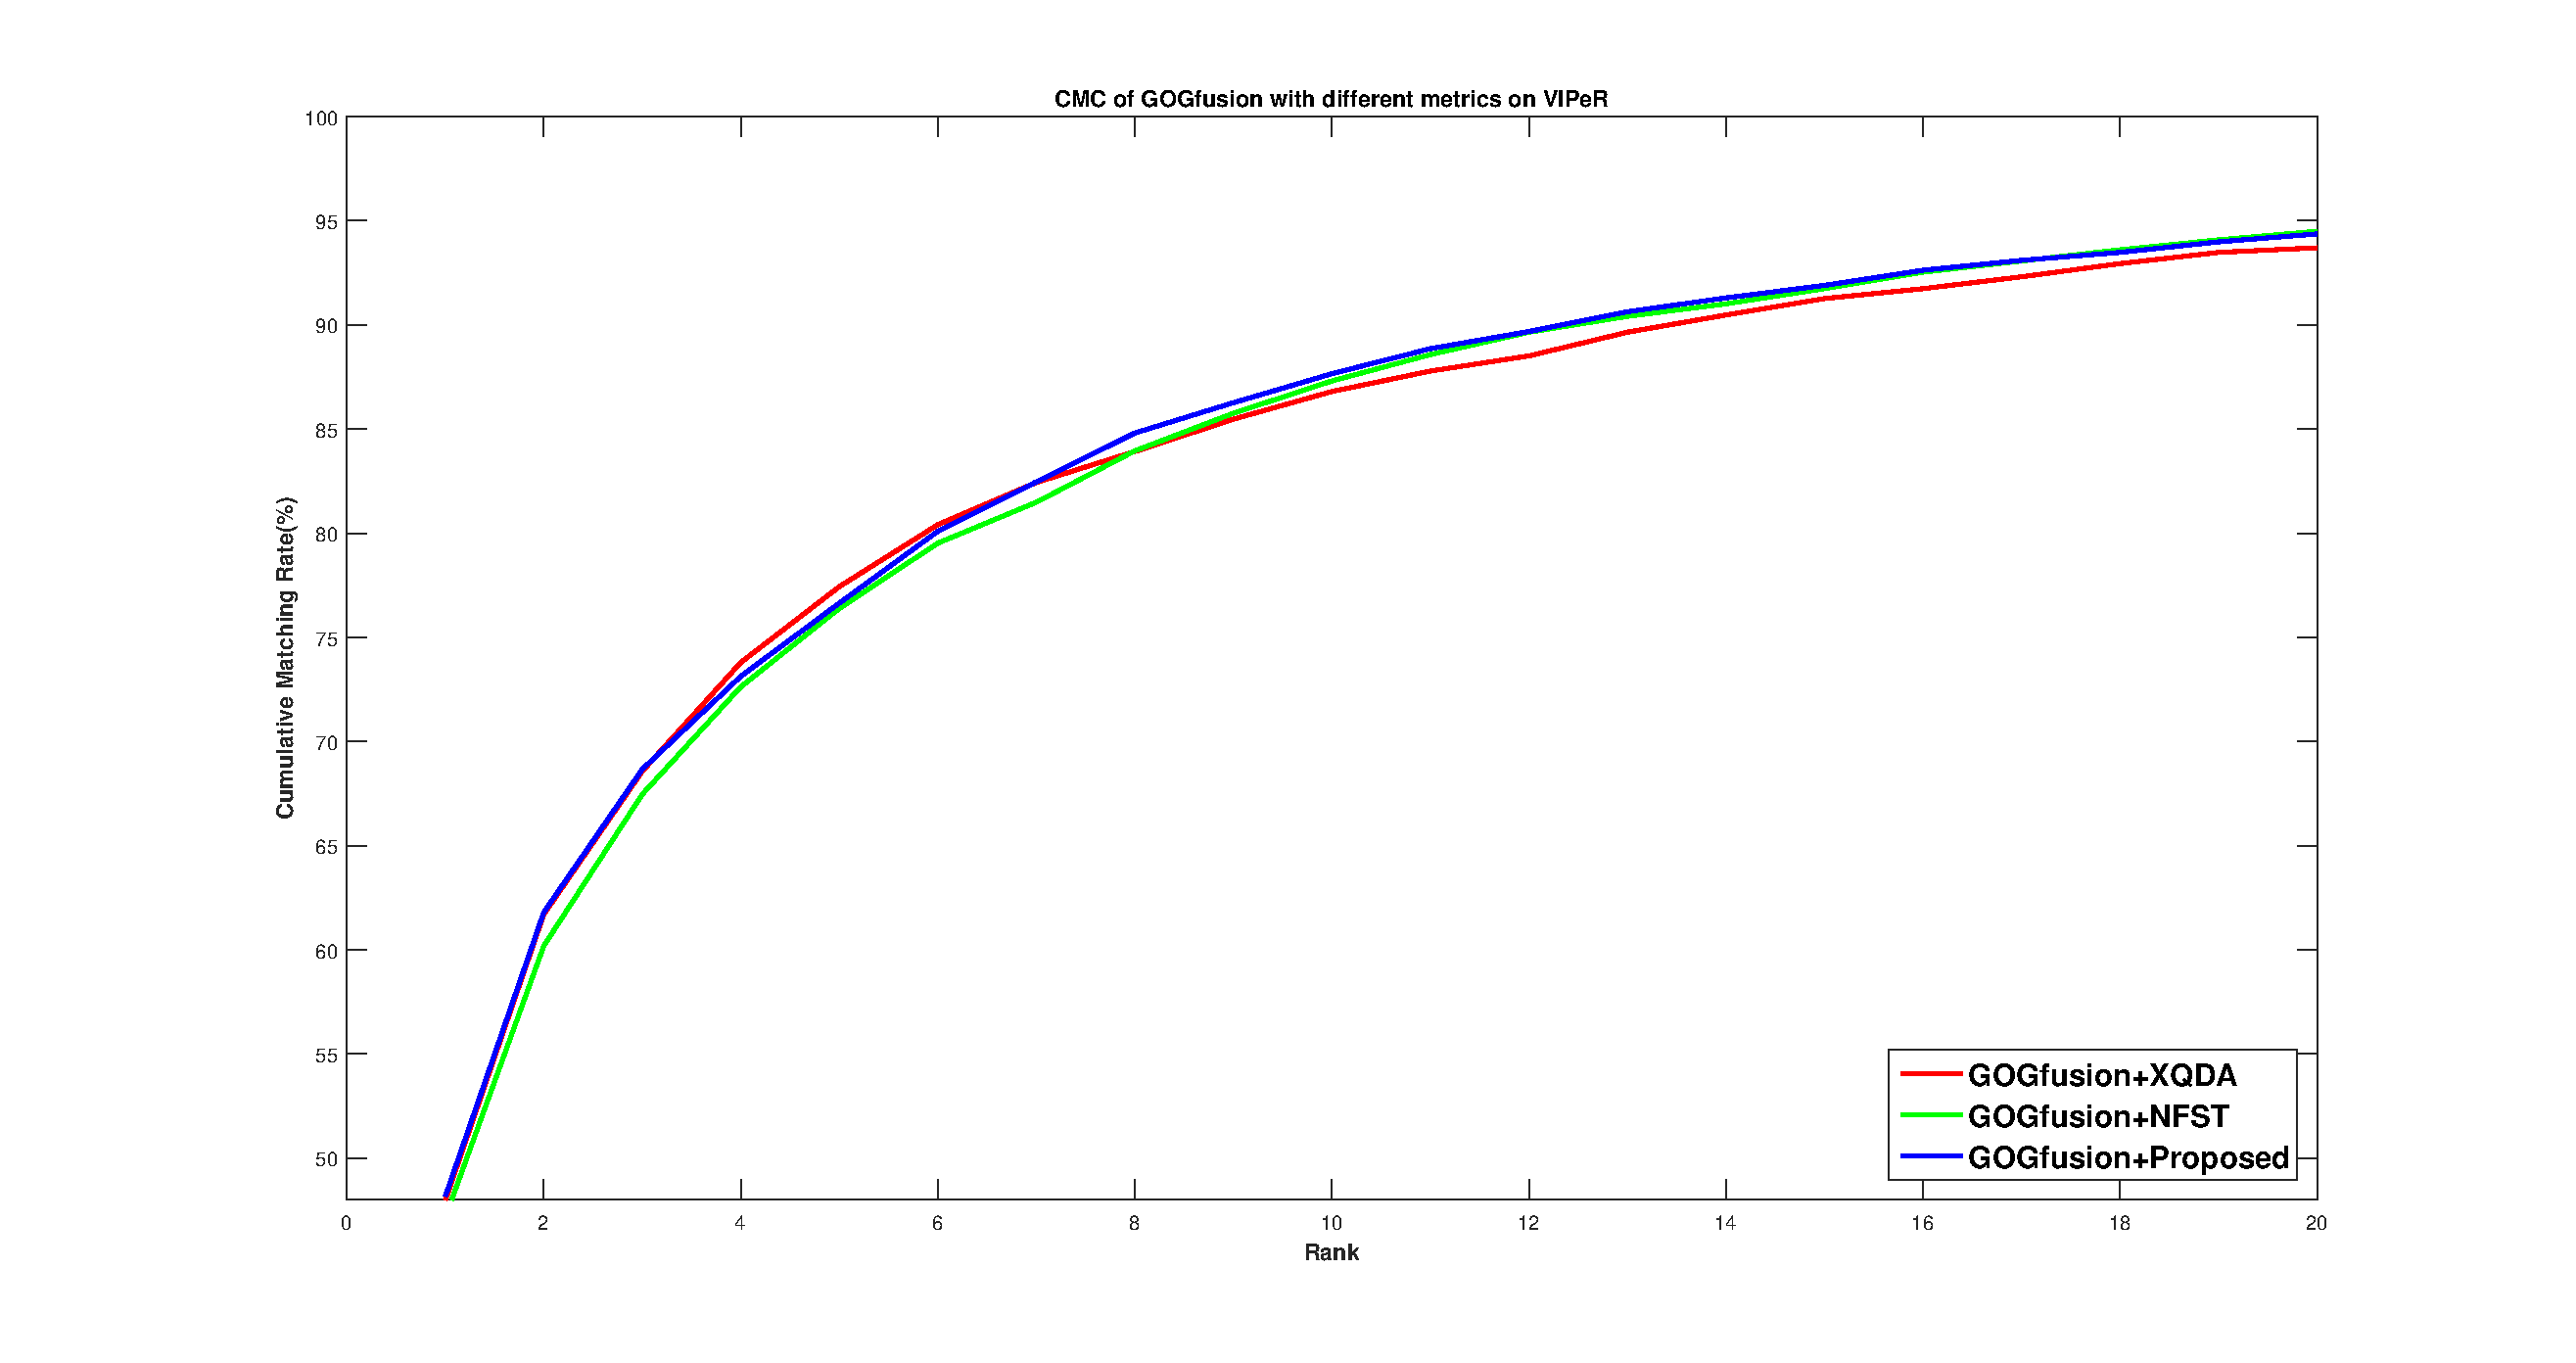
\includegraphics[width=1\linewidth]{/Users/JohnsonJohnson/Downloads/thesis_1/Figures/VIPeR.eps}
\vspace{-3em}
\caption{CMC curves on VIPeR comparing different metric learning}
\end{raggedleft}
\end{figure}
%-------------------------------

%-----------------------------------------------------------------------CUHK1
\begin{table}[H]
\caption{Performance of different metrics on CUHK1}
\centering
\begin{tabular}{|l|c|c|c|c|c|c|}
\hline
& \multicolumn{5}{|c|}{Rank(\%)} \\
\hline
Methods& 1 & 5 &10&15& 20\\
\hline
GOG$_\text{rgb}$+NFST&55.60 &83.02 &89.07 &91.98&93.56 \\ 
\hline
GOG$_\text{rgb}$+XQDA&50.51 &80.06 &87.10 &90.99&93.21 \\ 
\hline
%GOG$_\text{rgb}$+KLFDA&55.66&84.32&90.66&93.07& 94.63\\
%\hline
GOG$_\text{rgb}$+Proposed&55.91&84.24&90.41& 93.15&94.67\\  %55.86%, 84.28%, 90.45%, 93.09%, 94.65% 
\hline
GOG$_\text{fusion}$+NFST&56.26 &83.66 &89.63 &92.22&93.70 \\ 
\hline
GOG$_\text{fusion}$+XQDA&52.10 &81.85&88.81 &91.98&94.01\\ 
\hline
%GOG$_\text{fusion}$+KLFDA & 56.60&84.67&90.41&93.13&94.81\\
%\hline
GOG$_\text{fusion}$+Proposed&56.67&84.49& 90.51& 93.31&94.84\\
\hline
\end{tabular}\newline
\end{table}


\begin{figure}[H]
\centering
%\begin{raggedleft}
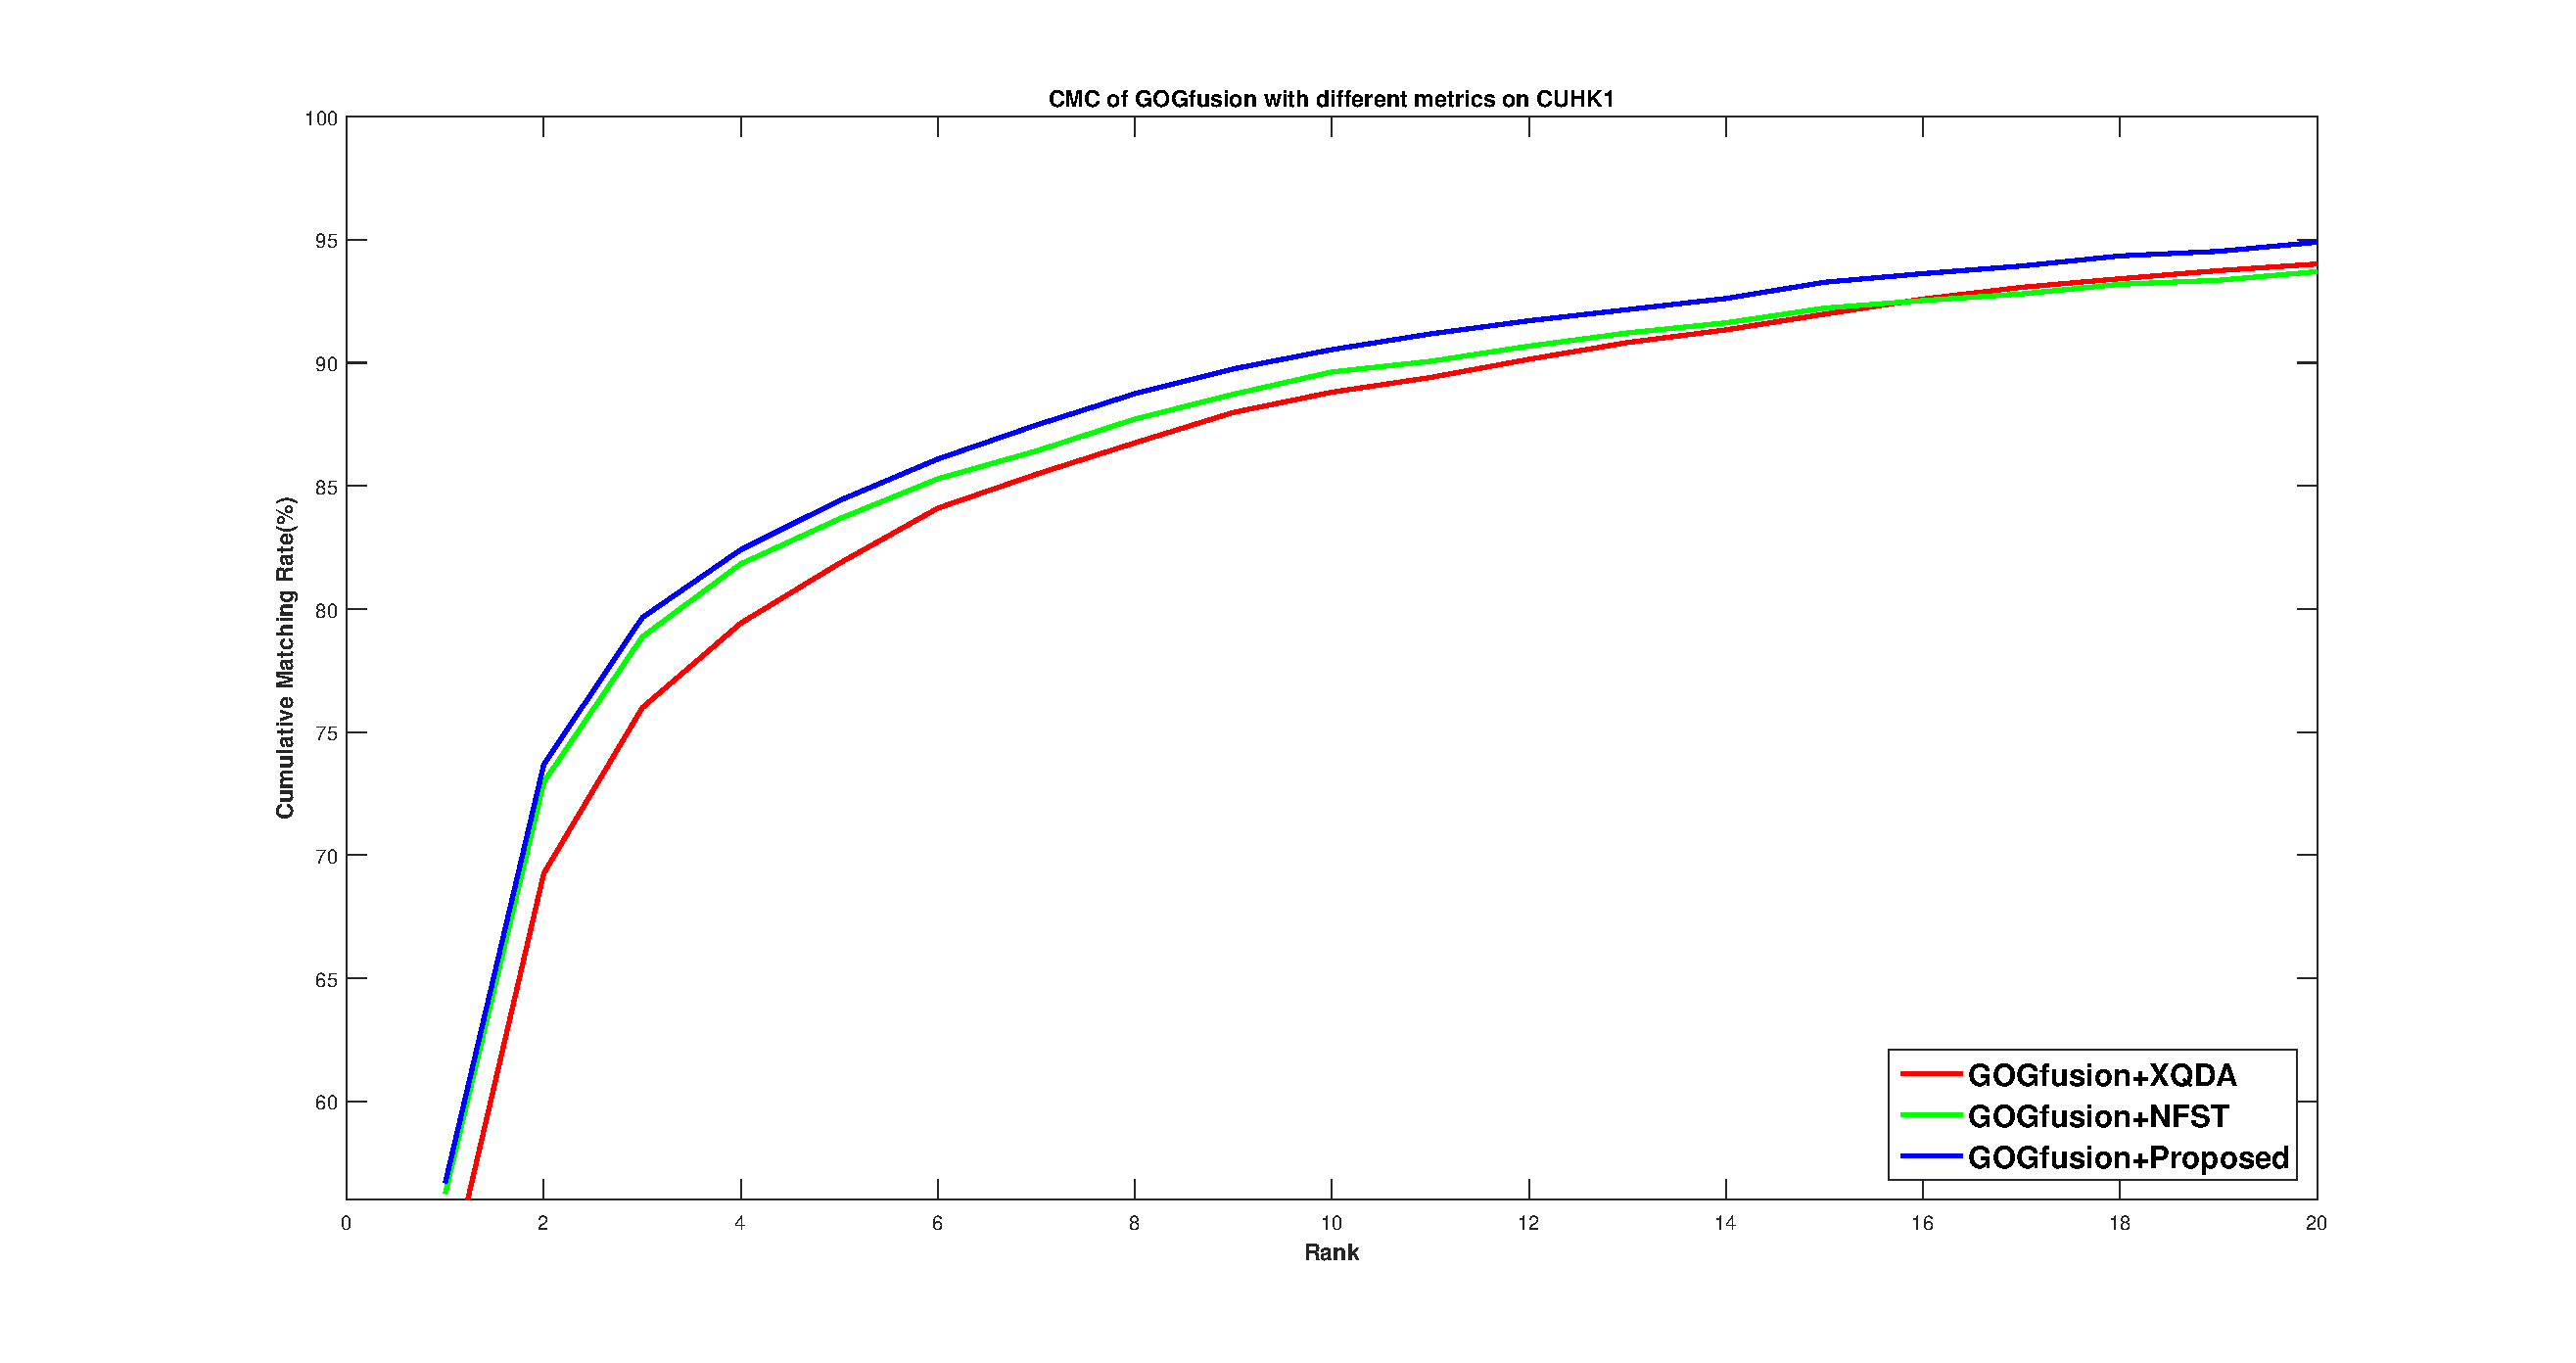
\includegraphics[width=1\linewidth]{/Users/JohnsonJohnson/Downloads/thesis_1/Figures/CUHK1.eps}
\vspace{-3em}
\caption{CMC curves on CUHK1 comparing different metric learning}
%\end{raggedleft}
\end{figure}

%-----------------------------------------------------------------------PRID_2011


\begin{table}[H]
\centering
\caption{Performance of different metrics on prid\_2011}
\begin{tabular}{|l|c|c|c|c|c|c|}
\hline
& \multicolumn{5}{|c|}{Rank(\%)} \\
\hline
Methods& 1 & 5 &10& 15&20\\
\hline
GOG$_\text{rgb}$+NFST&26.60 &53.80& 62.90&71.30&75.40 \\ 
\hline
GOG$_\text{rgb}$+XQDA&31.10 & 55.70& 66.10 & 72.40&76.10\\  
\hline
%GOG$_\text{rgb}$+KLFDA&23.70&51.70&63.10&69.90&73.60\\ 
%\hline
GOG$_\text{rgb}$+Proposed&23.80&52.20&63.50&70.20&73.50\\  %23.80%, 52.10%, 63.50%, 70.20%, 73.50%
\hline
GOG$_\text{fusion}$+NFST&34.10 &58.30& 67.60&73.80&78.30 \\  
\hline
GOG$_\text{fusion}$+XQDA&38.40& 61.30&70.80&75.60&79.30\\
\hline
%GOG$_\text{fusion}$+KLFDA & 31.90&56.90&66.60&72.60&77.50\\
%\hline
GOG$_\text{fusion}$+Proposed&32.30&57.40&66.30&73.40&78.00\\ %32.20%, 57.50%, 66.40%, 73.50%, 78.00(alpha = 0.7)   ()% 32.20%, 57.50%, 66.40%, 73.50%, 78.00%(alpha = 0.8)

\hline

\end{tabular}\newline
\end{table}

\textbf{Prid\_2011}  The  rank 1, rank5, rank 10, rank 15, rank 20 score of GOG$_\text{fusion}$  combined with proposed metric are 6.1\%, 3.9\%, 4.5\%, 2.2\% and 1.3\% lower than GOG$_\text{fusion}$ combined with XQDA. The performance of NFST is slightly better than proposed metric. Also in terms of GOG$_\text{rgb}$ XQDA and NFST has better performance than the proposed one. So in this dataset the proposed metric has worse performance than XQDA and NFST.

\begin{figure}[H]
\begin{raggedleft}
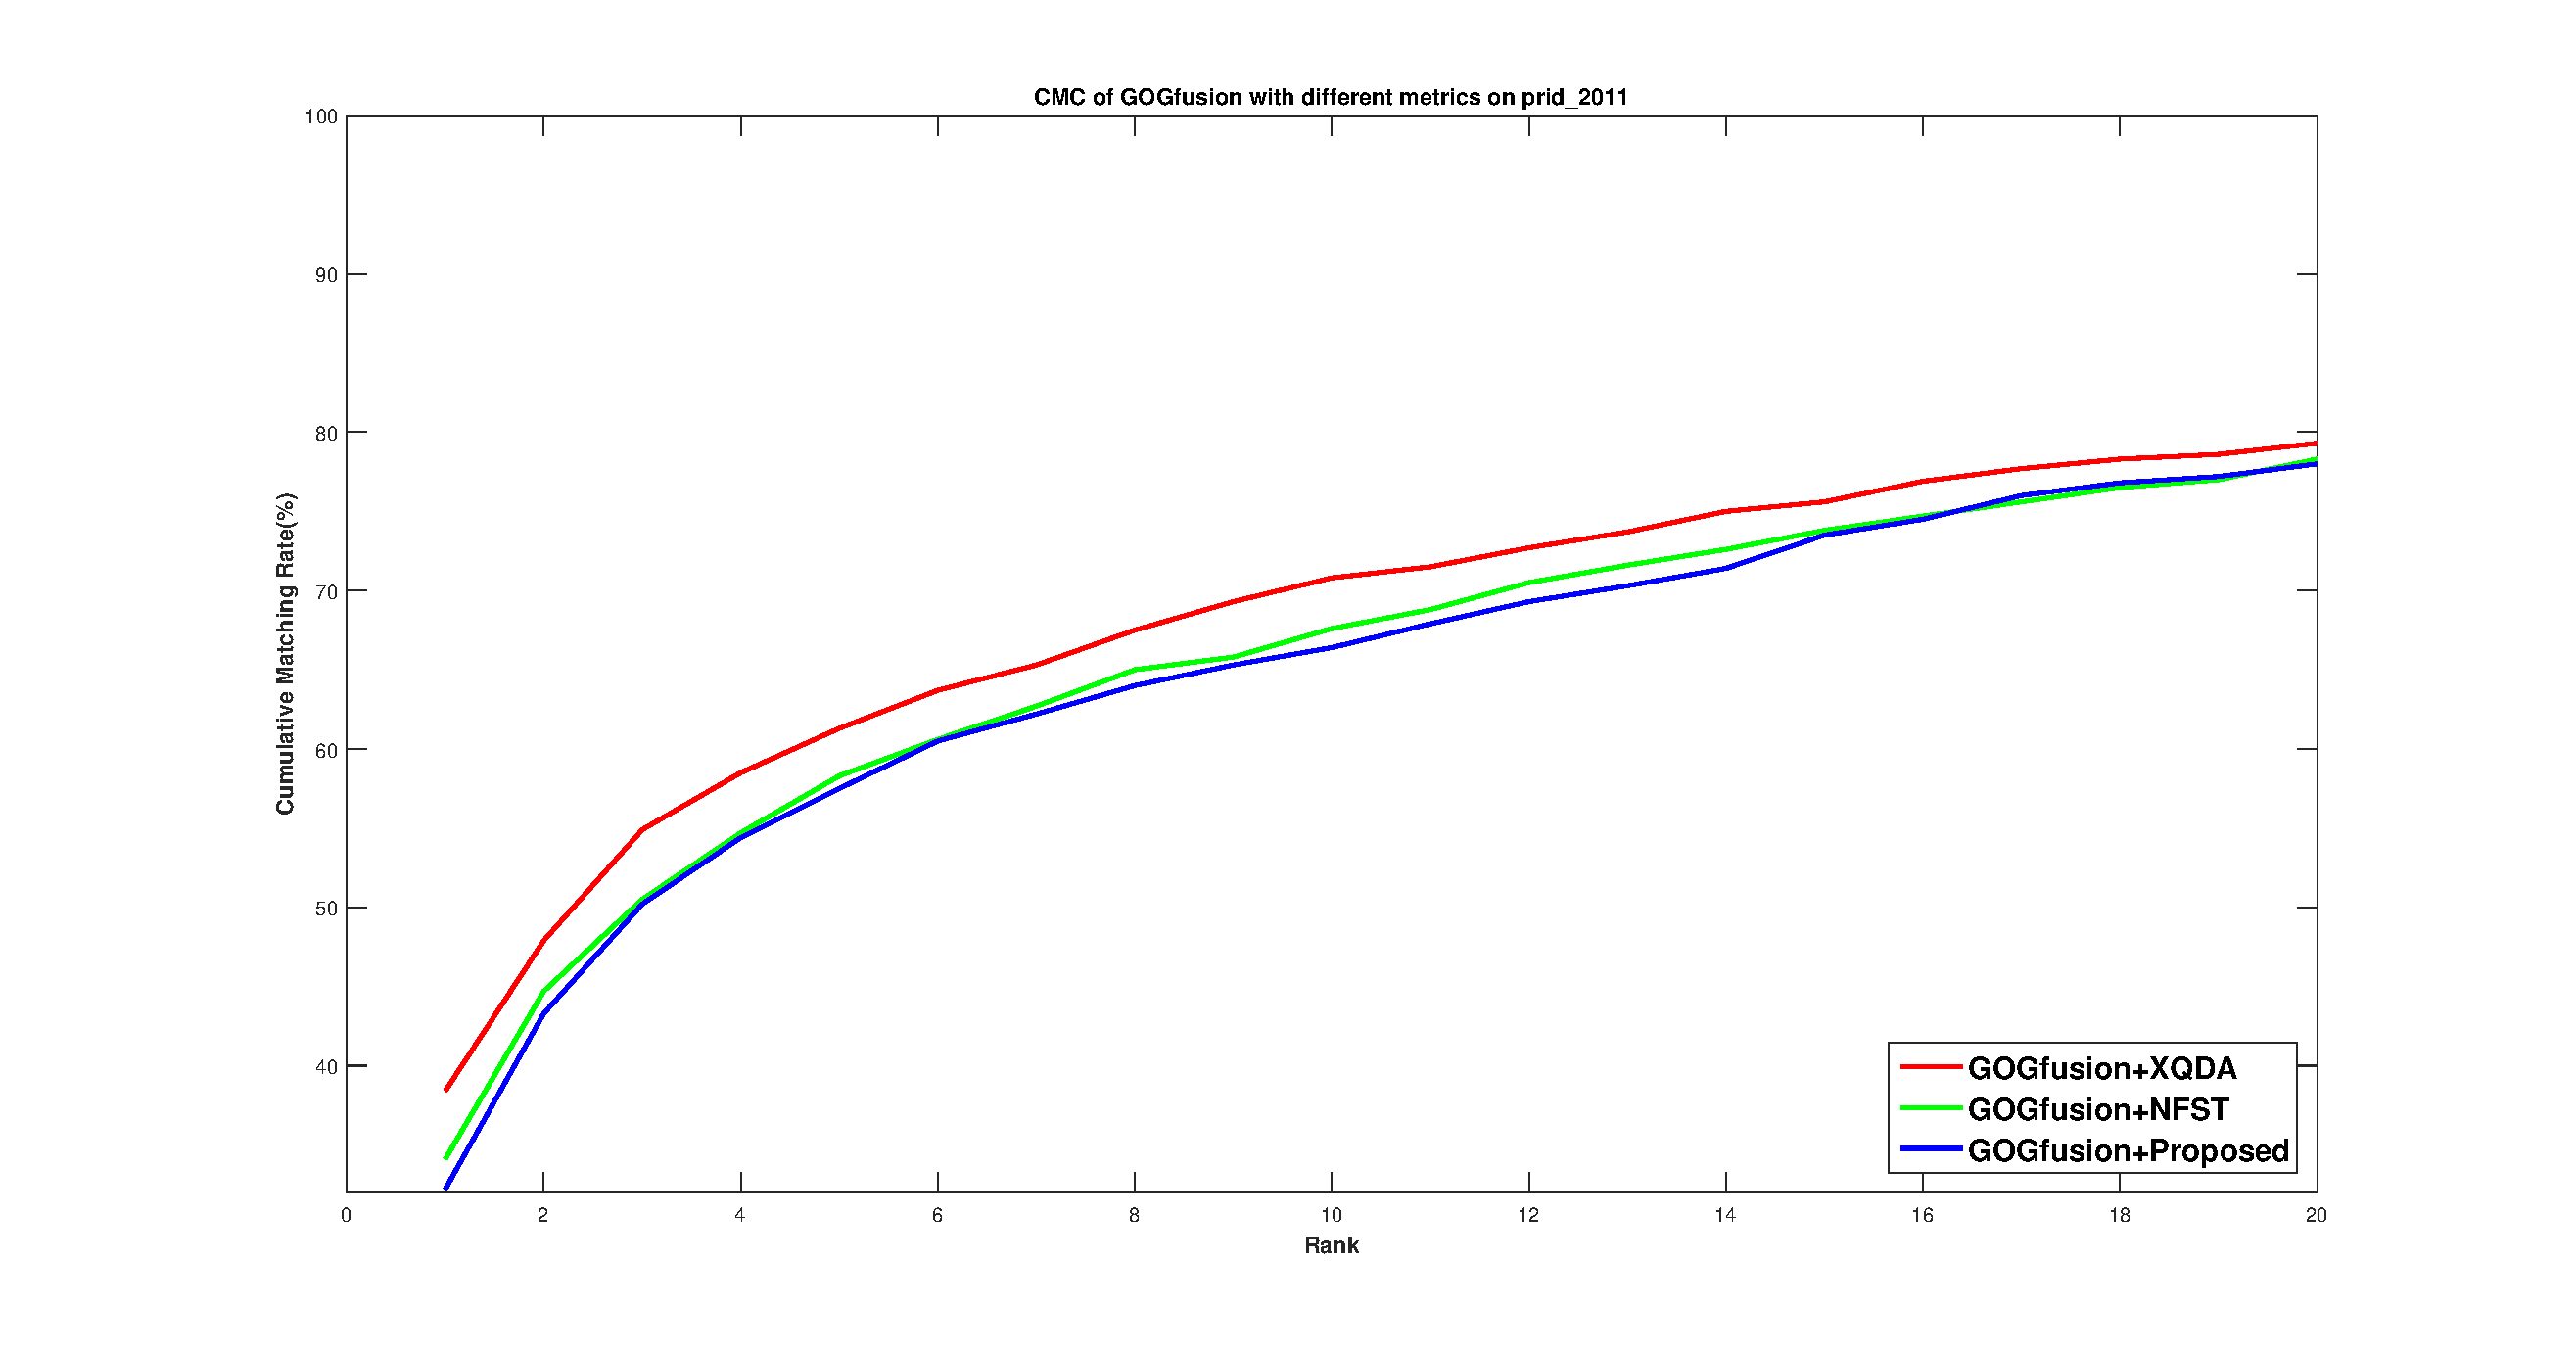
\includegraphics[width=1\linewidth]{/Users/JohnsonJohnson/Downloads/thesis_1/Figures/prid2011.eps}
\vspace{-3em}
\caption{CMC curves on prid\_2011 comparing different metric learning}
\end{raggedleft}
\end{figure}

%-----------------------------------------------------------------------PRID_450S
\begin{table}[H]
\caption{Performance of different metrics on prid\_450s}
\centering
\begin{tabular}{|l|c|c|c|c|c|c|}
\hline
& \multicolumn{5}{|c|}{Rank(\%)} \\
\hline
Methods& 1 & 5 &10& 15&20\\
\hline
GOG$_\text{rgb}$+NFST& 61.96&84.98 &90.53& 94.09&96.09 \\  %61.96%, 84.98%, 90.53%, 94.09%, 96.09%
\hline
GOG$_\text{rgb}$+XQDA&65.29 &85.02 & 91.13&94.76& 96.49\\ 
\hline
%GOG$_\text{rgb}$+KLFDA&60.04&84.09&90.93&94.04&96.00 \\ 
%\hline
GOG$_\text{rgb}$+Proposed&60.71&84.53&91.29&94.13&96.27\\  %60.44%, 84.44%, 91.33%, 94.00%, 96.13%
\hline
GOG$_\text{fusion}$+NFST& 64.53&86.62 & 92.93&95.78&97.42 \\ 
\hline
GOG$_\text{fusion}$+XQDA&68.40 & 87.42&93.47 &95.69& 97.02\\ 
\hline
%GOG$_\text{fusion}$+KLFDA & 62.58&86.18&92.18&95.11&96.84\\
%\hline
GOG$_\text{fusion}$+Proposed&62.80&86.58&92.36&95.29& 96.89\\ % 62.62%, 86.44%, 92.36%, 95.20%, 96.93%(alpha = 0.7) 62.89%, 86.49%, 92.49%, 95.29%, 97.07%(alpha = 0.8)

\hline

\end{tabular}
\end{table}
\textbf{Prid\_450s} In this dataset, we can find the rank 1 score of XQDA and NFST is higher than proposed metric, but they have almost the same rank 5, rank 10, rank 15, and rank 20 scores with respect to both kinds of descriptors.  

\begin{figure}[H]
\begin{raggedleft}
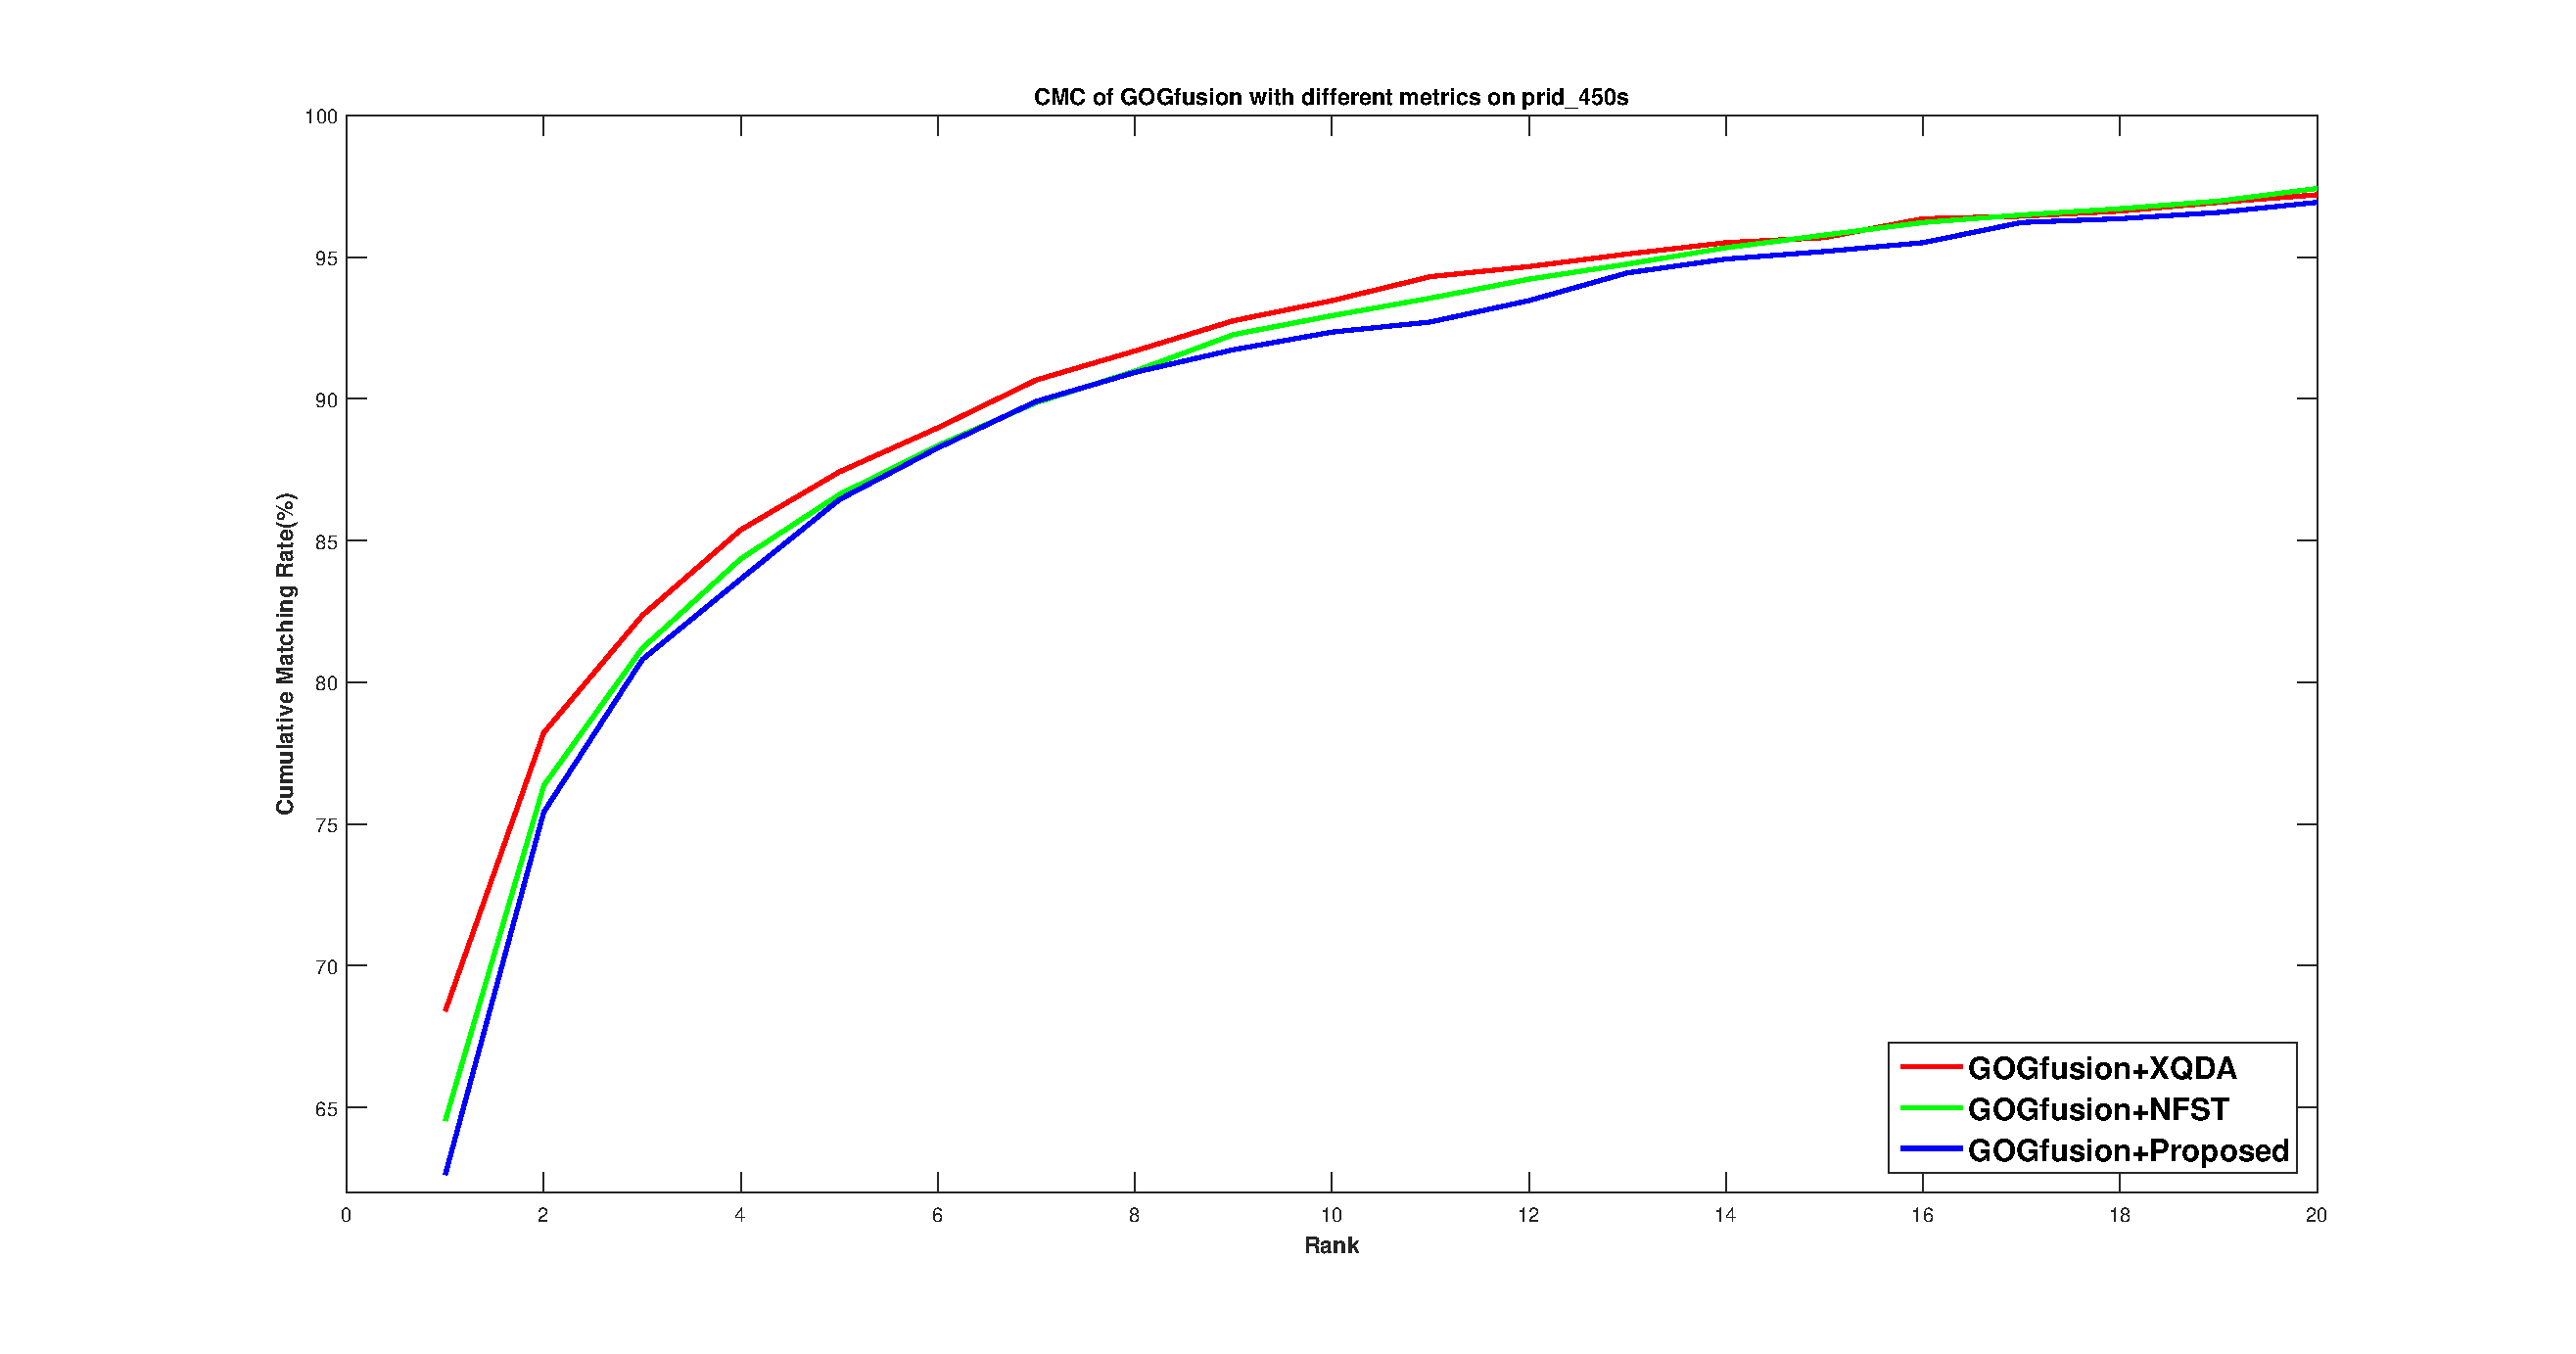
\includegraphics[width=1\linewidth]{/Users/JohnsonJohnson/Downloads/thesis_1/Figures/prid450s.eps}
\vspace{-3em}
\caption{CMC curves on prid\_450s comparing different metric learning}
\end{raggedleft}
\end{figure}

%-----------------------------------------------------------------------GRID
\begin{table}[H]
\caption{Performance of different metrics on GRID}
\centering
\begin{tabular}{|l|c|c|c|c|c|c|}
\hline
& \multicolumn{5}{|c|}{Rank(\%)} \\
\hline
Methods& 1 & 5 &10& 15&20\\
\hline
GOG$_\text{rgb}$+NFST& 21.84&41.28 &50.96& 57.44&62.88 \\ 
\hline
GOG$_\text{rgb}$+XQDA& 22.64&43.92 &55.12 &61.12&66.56\\ 
\hline
%GOG$_\text{rgb}$+KLFDA&23.44&43.04&52.16&59.12&64.88 \\ 
%\hline
GOG$_\text{rgb}$+Proposed&22.64&43.68&52.00&59.04&65.04\\  %22.80%, 43.76%, 52.08%, 59.04%, 65.12%
\hline
GOG$_\text{fusion}$+NFST& 23.04&44.40 &54.40 &61.84&66.56\\ 
\hline
GOG$_\text{fusion}$+XQDA& 23.68&47.28 &58.40 &65.84&69.68 \\ 
\hline
%GOG$_\text{fusion}$+KLFDA &23.76&44.40& 55.36&61.76& 66.48\\
%\hline
GOG$_\text{fusion}$+Proposed&23.92&44.64&54.88&62.32&66.40\\ %23.84%, 44.64%, 55.04%, 62.24%, 66.24%

\hline

\end{tabular}
\end{table}

\begin{figure}[H]
\begin{raggedleft}
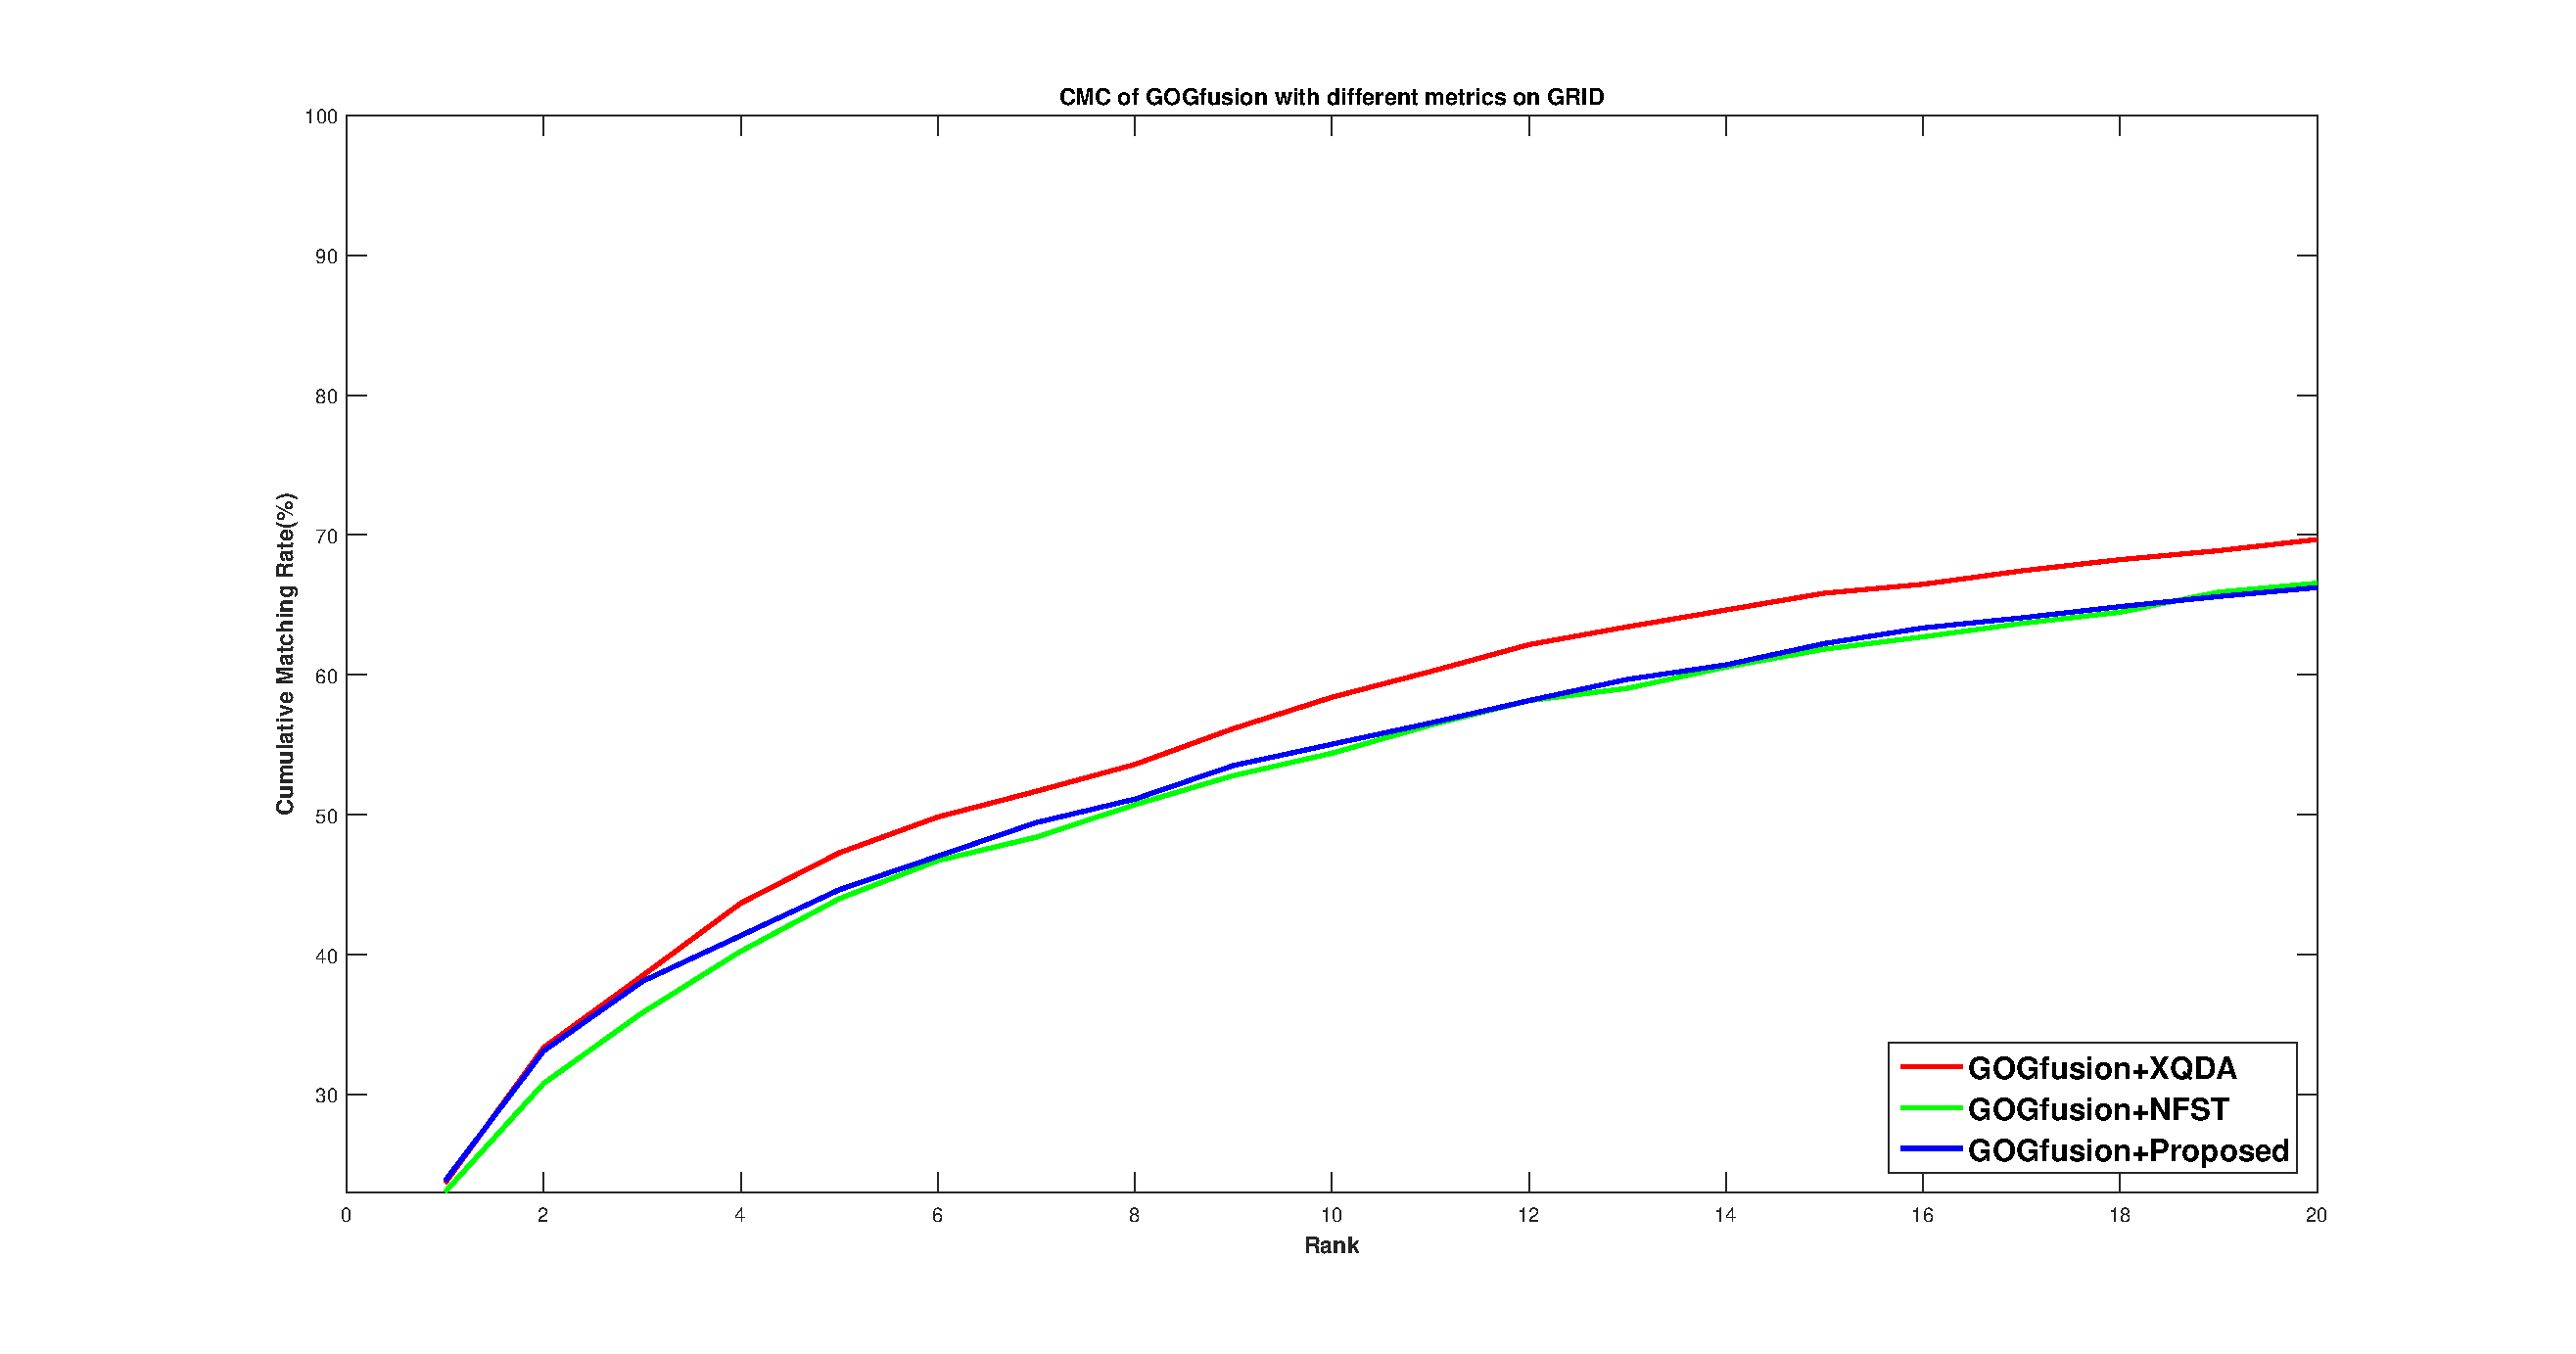
\includegraphics[width=1\linewidth]{/Users/JohnsonJohnson/Downloads/thesis_1/Figures/GRID.eps}
\vspace{-3em}
\caption{CMC curves on GRID comparing different metric learning}
\end{raggedleft}
\end{figure}

\textbf{GRID} We can see that the rank 1 score of proposed metric are 0.24\% higher than XQDA and 0.88\% higher than NFST in terms of GOG$_\text{fusion}$, but XQDA outperforms proposed metric on rank 5, rank 10, rank 15 and rank 20 scores. Besides, proposed metric outperforms NFST on rank 5, rank 10, rank 15 scores.\\
\indent In summary, the Re-ID performance is improved in VIPeR, CUHK01 dataset, and has almost the same performance with NFST and XQDA on prid\_450s dataset. Specifically, proposed metric learning has the best rank 1 score in GRID dataset and its performance is only second to XQDA. The proposed metric has superior performance for following reasons: (1) dimension reduction by KLFDA exploits the nonlinearity and the loss of discriminant information between classes are minimized. (2) the simplified relative distance limitation optimization helps to confine the Mahanalobis distance matrix $\bm{M}$ to discriminate different classes.  
%------------------------------------------------------------------------

 
% Chapter Template

\chapter{Conclusion} % Main chapter title

%\label{ChapterX} % Change X to a consecutive number; for referencing this chapter elsewhere, use \ref{ChapterX}
%\section{}
In this thesis, KLFDA was used to reduce the dimension of the hierarchical Gaussian descriptors, and gradient descent method was used to learn a Mahalanobis distance matrix on a lower-dimensional space. By comparison, we found that the proposed metric has better performance than NFST and XQDA on the VIPeR and CUHK1 datasets, but XQDA and NFST outperformed the proposed metric learning on the Prid\_2011 and Prid\_450s. We also found that the proposed metric learning had better rank 1 score than NFST, and its performance was only second to XQDA on the GRID dataset. 
\section{Contributions}
There are three contributions in this thesis. (1) The metric learning on the dimension-reduced hierarchical Gaussian descriptor by KLFDA has been studied. The gradient descent method optimizes the Mahalanobis distance matrix on the lower-dimensional space. It has been demonstrated that extra improvements can be achieved in this lower-dimensional space. (2) The influence of background and foreground segmentation on different descriptors has also been studied. The results are that foreground segmentation improves performance of color-based descriptors but decreases performance of texture-based descriptors, which is caused by imperfect segmentation on single-image-based foreground segmentation. (3) Some variants of the hierarchical Gaussian descriptor have been tested. LBP and superpixel segmentation were combined with the hierarchical Gaussian descriptor, but those variants had worse performance than the original hierarchical Gaussian descriptor.
\section{Future work}
\subsection{Improve the hierarchical Gaussian descriptor}
It has been demonstrated that in the basic pixel feature $\bm{f}_i$, the color components are more important than the $y$ coordinate and gradient components. LBP has been proven to be a worse choice for texture representation in $\bm{f}_i$. Therefore, one strategy to improve the hierarchical Gaussian descriptor is to find a better texture representation to replace gradient components in basic pixel feature. 
\subsection{Influence of video-based foreground segmentation}
Though the single-image-based foreground and background segmentation's influence on different descriptors has been studied, extra effort is needed to study sequence-based or video-based foreground segmentation's influence on different descriptors. Video-based foreground often has better results. If the background can be well modelled by a video or a sequence of images so that less textural noise is created, the segmentation might improve the hierarchical Gaussian descriptor's performance.
\subsection{Computational cost of gradient descent method}
It is important to reduce the computational cost of the gradient descent method. It takes an average of about average 15 iterations when training the Mahalanobis distance matrix. The training time for a larger dataset, like the CUHK1 dataset, takes up to one hour on a computer with a 16GB RAM, Intel i5 processor. Therefore, other variants of gradient the descent method, like stochastic gradient method and conjugate gradient method, may be tested for lower computational cost.


%----------------------------------------------------------------------------------------
%	SECTION 1
%----------------------------------------------------------------------------------------

%\section{Main Section 1}
%
%Lorem ipsum dolor sit amet, consectetur adipiscing elit. Aliquam ultricies lacinia euismod. Nam tempus risus in dolor rhoncus in interdum enim tincidunt. Donec vel nunc neque. In condimentum ullamcorper quam non consequat. Fusce sagittis tempor feugiat. Fusce magna erat, molestie eu convallis ut, tempus sed arcu. Quisque molestie, ante a tincidunt ullamcorper, sapien enim dignissim lacus, in semper nibh erat lobortis purus. Integer dapibus ligula ac risus convallis pellentesque.
%
%%-----------------------------------
%%	SUBSECTION 1
%%-----------------------------------
%\subsection{Subsection 1}
%
%Nunc posuere quam at lectus tristique eu ultrices augue venenatis. Vestibulum ante ipsum primis in faucibus orci luctus et ultrices posuere cubilia Curae; Aliquam erat volutpat. Vivamus sodales tortor eget quam adipiscing in vulputate ante ullamcorper. Sed eros ante, lacinia et sollicitudin et, aliquam sit amet augue. In hac habitasse platea dictumst.
%
%%-----------------------------------
%%	SUBSECTION 2
%%-----------------------------------
%
%\subsection{Subsection 2}
%Morbi rutrum odio eget arcu adipiscing sodales. Aenean et purus a est pulvinar pellentesque. Cras in elit neque, quis varius elit. Phasellus fringilla, nibh eu tempus venenatis, dolor elit posuere quam, quis adipiscing urna leo nec orci. Sed nec nulla auctor odio aliquet consequat. Ut nec nulla in ante ullamcorper aliquam at sed dolor. Phasellus fermentum magna in augue gravida cursus. Cras sed pretium lorem. Pellentesque eget ornare odio. Proin accumsan, massa viverra cursus pharetra, ipsum nisi lobortis velit, a malesuada dolor lorem eu neque.
%
%%----------------------------------------------------------------------------------------
%%	SECTION 2
%%----------------------------------------------------------------------------------------
%
%\section{Main Section 2}
%
%Sed ullamcorper quam eu nisl interdum at interdum enim egestas. Aliquam placerat justo sed lectus lobortis ut porta nisl porttitor. Vestibulum mi dolor, lacinia molestie gravida at, tempus vitae ligula. Donec eget quam sapien, in viverra eros. Donec pellentesque justo a massa fringilla non vestibulum metus vestibulum. Vestibulum in orci quis felis tempor lacinia. Vivamus ornare ultrices facilisis. Ut hendrerit volutpat vulputate. Morbi condimentum venenatis augue, id porta ipsum vulputate in. Curabitur luctus tempus justo. Vestibulum risus lectus, adipiscing nec condimentum quis, condimentum nec nisl. Aliquam dictum sagittis velit sed iaculis. Morbi tristique augue sit amet nulla pulvinar id facilisis ligula mollis. Nam elit libero, tincidunt ut aliquam at, molestie in quam. Aenean rhoncus vehicula hendrerit.

%----------------------------------------------------------------------------------------
%	THESIS CONTENT - APPENDICES
%----------------------------------------------------------------------------------------

\appendix % Cue to tell LaTeX that the following "chapters" are Appendices

% Include the appendices of the thesis as separate files from the Appendices folder
% Uncomment the lines as you write the Appendices

% Appendix A

\chapter{Frequently Asked Questions} % Main appendix title

\label{AppendixA} % For referencing this appendix elsewhere, use \ref{AppendixA}

\section{How do I change the colors of links?}

The color of links can be changed to your liking using:

{\small\verb!\hypersetup{urlcolor=red}!}, or

{\small\verb!\hypersetup{citecolor=green}!}, or

{\small\verb!\hypersetup{allcolor=blue}!}.

\noindent If you want to completely hide the links, you can use:

{\small\verb!\hypersetup{allcolors=.}!}, or even better: 

{\small\verb!\hypersetup{hidelinks}!}.

\noindent If you want to have obvious links in the PDF but not the printed text, use:

{\small\verb!\hypersetup{colorlinks=false}!}.

%\include{Appendices/AppendixB}
%\include{Appendices/AppendixC}

%----------------------------------------------------------------------------------------
%	BIBLIOGRAPHY
%----------------------------------------------------------------------------------------

\printbibliography[heading=bibintoc]

%----------------------------------------------------------------------------------------

\end{document}  
